\documentclass[a4paper, 11pt]{memoir}

\usepackage[T1]{fontenc}
\usepackage[utf8]{inputenc}

\usepackage[english]{babel}

%
% Smart Thesis LaTeX template
%
% [To underline the amateurish flavour of this template, let's start with some
% nifty ASCII-Art (http://www.network-science.de/ascii/)...]
%
%      #######
%    /       ###
%   /         ##                                          #
%   ##        #                                          ##
%    ###                                                 ##
%   ## ###      ### /### /###     /###   ###  /###     ########
%    ### ###     ##/ ###/ /##  / / ###  / ###/ #### / ########
%      ### ###    ##  ###/ ###/ /   ###/   ##   ###/     ##
%        ### /##  ##   ##   ## ##    ##    ##            ##
%          #/ /## ##   ##   ## ##    ##    ##            ##
%           #/ ## ##   ##   ## ##    ##    ##            ##
%            # /  ##   ##   ## ##    ##    ##            ##
%  /##        /   ##   ##   ## ##    /#    ##            ##
% /  ########/    ###  ###  ### ####/ ##   ###           ##
%/     #####       ###  ###  ### ###   ##   ###           ##
%|
% \)
%
%
%  /###           /  /
% /  ############/ #/                              #
%/     #########   ##                             ###
%#     /  #        ##                              #
% ##  /  ##        ##
%    /  ###        ##  /##      /##       /###   ###        /###
%   ##   ##        ## / ###    / ###     / #### / ###      / #### /
%   ##   ##        ##/   ###  /   ###   ##  ###/   ##     ##  ###/
%   ##   ##        ##     ## ##    ### ####        ##    ####
%   ##   ##        ##     ## ########    ###       ##      ###
%    ##  ##        ##     ## #######       ###     ##        ###
%     ## #      /  ##     ## ##              ###   ##          ###
%      ###     /   ##     ## ####    /  /###  ##   ##     /###  ##
%       ######/    ##     ##  ######/  / #### /    ### / / #### /
%         ###       ##    ##   #####      ###/      ##/     ###/
%                         /
%                        /
%                       /
%                      /
%
% About:
% ======
%
% This template is a re-implementation of the "classicthesis" template by André
% Miede. However, it uses the "memoir" class as a basis, eliminating most
% of the external packages required by "classicthesis" and thus (hopefully)
% achieving a higher compatibility with other LaTeX packages. Large parts of
% the code have been adapted (ransacked) from André Miedes code.
%
% You can find more information about "classicthesis" at CTAN:
%
% https://www.ctan.org/pkg/classicthesis
%
% More information about the "memoir" package can be found here:
%
% https://www.ctan.org/pkg/memoir
%
%
% Authors:
% ========
%
% Jan Philip Göpfert, Andreas Stöckel
%
%
% License:
% ========
%
% This LaTeX template is published under the Creative Commons Zero license. To
% the extent possible under law, the authors have waived all copyright and
% related neighboring rights to Smart Thesis. This work is published from:
% Germany.
%


%
% EXTERNAL PACKAGES
%
\usepackage[usenames,dvipsnames,svgnames]{xcolor}
\usepackage{ragged2e} % for marginnote

%
% FONT DEFINITIONS
%

% Use the following code for XeLaTeX
\ifxetex

% Setup microtype for XeLaTeX
\usepackage[expansion=false,final]{microtype}

% Load the texgyrepagella font as main font and set the ``mathpazo'' font as
% math font
\usepackage{fontspec}
\usepackage{mathpazo}
\setmainfont%
	[%
		BoldFont       = texgyrepagella-bold.otf,
		ItalicFont     = texgyrepagella-italic.otf,
		BoldItalicFont = texgyrepagella-bolditalic.otf,
		Ligatures      = TeX
	]%
	{texgyrepagella-regular.otf}

% Define a new 'widespaced' font that is used in section headings
% or chapter titles. For backwards compatibility reasons this uses
% the old calling convention \newfontfamily\fontname[<options>{font}
% instead of the newer \newfontfamily\fontname{font}[<options>]
\newfontfamily\widespaced[%
	LetterSpace=15,%
	WordSpace={1.25, 1.25, 1.25}%
]{texgyrepagella-regular.otf}%

\DeclareRobustCommand{\spacedallcaps}[1]{%
	{\widespaced\oldstylenums{\MakeTextUppercase{#1}}}%
}%
\DeclareRobustCommand{\spacedlowsmallcaps}[1]{%
	{\widespaced\oldstylenums{\textsc{\MakeTextLowercase{#1}}}}%
}%
\fi

% Use the following code for pdfLaTex
\ifpdf

% Setup microtype for pdfLaTex
\usepackage[final,tracking=true,kerning=true,spacing=nonfrench]{microtype}


\usepackage[sc]{mathpazo}

\DeclareRobustCommand{\spacedallcaps}[1]{\textls[160]{\oldstylenums{\textsc{\MakeTextUppercase{#1}}}}}%
\DeclareRobustCommand{\spacedlowsmallcaps}[1]{\textls[80]{\oldstylenums{\textsc{\MakeTextLowercase{#1}}}}}%
\fi

% Increase linespread for Palatino
\renewcommand{\linespread}{1.05}

%
% COLOR DEFINITIONS
%

\definecolor{smartgray}{gray}{0.55}
\definecolor{smartred}{HTML}{800000}
\definecolor{smartplum}{HTML}{47294F}
\definecolor{smartblue}{HTML}{193A6B}
\definecolor{smartorange}{HTML}{AA4C00}
\definecolor{smartgreen}{HTML}{3C7705}
\definecolor{smartbutter}{HTML}{A08300}

\definecolor{tangored}{HTML}{CC0000}
\definecolor{tangoplum}{HTML}{75507B}
\definecolor{tangoblue}{HTML}{3465A4}
\definecolor{tangoorange}{HTML}{F57900}
\definecolor{tangogreen}{HTML}{73D216}
\definecolor{tangobutter}{HTML}{EDD400}

\definecolor{shadecolor}{gray}{0.95}

\colorlet{heading}{smartgray}
\colorlet{ref}{smartblue}
\colorlet{cite}{smartgreen}
\colorlet{url}{smartred}
\colorlet{caption}{black}
\colorlet{margincaption}{caption}

%
% SECTIONING STYLES (toledo)
%

% See http://tex.stackexchange.com/questions/161577/memoir-hangnum-chapter-number-in-right-margin-switch for the inspiration

\setsecnumdepth{subsection}

\makeatletter
\makechapterstyle{toledo}{%
	\chapterstyle{default}

	\renewcommand*{\chapterheadstart}{\vspace*{0.0cm}}

	\renewcommand*{\chapnumfont}{\normalfont\color{heading}\addfontfeature{SizeFeatures={Size=110}}}
	\newfont{\chapterNumber}{eurb10 scaled 7000}
	\renewcommand*{\chapnumfont}{\chapterNumber\color{heading}}
	\renewcommand*{\printchaptername}{}
	\renewcommand*{\chapternamenum}{}
	\renewcommand*{\printchapternum}{%
		\raisebox{0pt}[0pt][0pt]{%
		\makebox[0pt][l]{%
		\makebox[\dimexpr\textwidth+5.45em\relax][l]{%
			\parbox[t]{\textwidth}{\mbox{}}%
			\parbox[t]{5.45em}{\hfill\chapnumfont \thechapter}}}}}%
	\renewcommand*{\chapternamenum}{}
	\renewcommand*{\afterchapternum}{}

	\renewcommand*{\afterchaptertitle}{%
	\par\parbox{\textwidth}{\hrulefill}\par%
	\vspace*{4ex}}
	\renewcommand*{\chaptitlefont}{\normalfont\large}
	\renewcommand*{\printchaptertitle}[1]{%
		\parbox[b]{\textwidth}{%
			\raggedright\chaptitlefont\spacedallcaps{##1}%
		}%
	}

	\setsecheadstyle{\spacedlowsmallcaps}
	\setsecindent{-3.5ex}
	\setbeforesecskip{-4ex plus -1ex minus -.2ex}
	\setaftersecskip{4ex plus 1ex minus .2ex}

	\setsubsecheadstyle{\itshape}
	\setbeforesubsecskip{-4ex plus -1ex minus -.2ex}
	\setaftersubsecskip{4ex plus 1ex minus .2ex}
	\setsecnumformat{\spacedlowsmallcaps{\csname the##1\endcsname\quad}}

%	\setparaheadstyle{\normalsize\itshape}

	\renewcommand*{\abstractnamefont}{\spacedlowsmallcaps}
}
\makeatother

\chapterstyle{toledo}

%
% FIGURES
%

\captionstyle{\small}
\captionnamefont{\slshape\color{caption}}

\newsubfloat{figure}% Create subfloat in figure environment
\newsubfloat{table}% Create subfloat in table environment

%
% ACKNOWLEDGEMENT
%

\makeatletter
\newcommand{\acknowledgementname}{Acknowledgements}
\newenvironment{acknowledgement}{%
  \setup@bstract
  \if@bsrunin\else
    \ifnumber@bs \num@bs \else
      \begin{\absnamepos}\abstractnamefont\acknowledgementname\end\absnamepos%
      \vspace{\abstitleskip}%
    \fi
  \fi
  \put@bsintoc%
  \begin{@bstr@ctlist}\if@bsrunin\@bsrunintitle\fi\abstracttextfont}%
  {\par\end{@bstr@ctlist}}

\newcommand{\smartcopyright}[1]{\begingroup%
	\pagebreak%
	\thispagestyle{empty}%
	\footnotesize%
	\par\vspace*{\fill}%
	\hspace{-1.1cm}%
	\parbox{10cm}{%
		\noindent%
		Copyright \textcopyright\ \the\year\ \applytolist[, ]{}{\@author}\\[0.5cm]%
		{#1}%
	}%
\endgroup}

\newcommand{\smartinitialepigraph}[2]{\begingroup
	\cleardoublepage
	\thispagestyle{empty}
	\vspace*{2cm}
	\epigraph{#1}{#2}
	\cleardoublepage
\endgroup}

\let\oldepigraph\epigraph
\renewcommand{\epigraph}[2]{\oldepigraph{#1}{\spacedlowsmallcaps{#2}}}

\makeatother

%
% MARGINNOTE
%

%
% There are three commands for placing elements in the margin:
%
% \marginnote{<TEXT>}
% Just like \marginpar but with correct formating
%
% \marginfig{<SHORT CAPTION>}{<FIGURE CONTENT>}{<LONG CAPTION>}{\label{<LABEL>}}
% \margintbl{<SHORT CAPTION>}{<TABLE CONTENT>}{<LONG CAPTION>}{\label{<LABEL>}}
% Places a figure/table in the margin
% - <SHORT CAPTION> is the caption as it occurs in the list of figures/tables
% - <FIGURE CONTENT>/<TABLE CONTENT> is the actual figure/table content
% - <LONG CAPTION> is the caption below the figure
% - <LABEL> is the label -- we decided to let you explicitly type "\label" here
% as this allows LaTeX editors to index the label and provide auto completion.
%

% Define the "marginnote" command. For compatibility reasons
% we do not override marginpar.
\strictpagecheck
\newcommand{\marginnote}[1]{\hspace*{0pt}\marginpar{
	\microtypesetup{disable}%
	\slshape\footnotesize%
	\vspace*{-0.725em}%
	\checkoddpage%
	\ifoddpage%
		\RaggedRight%
	\else%
		\RaggedLeft%
	\fi%
	{#1}%
	\microtypesetup{enable}%
}\ignorespaces}

\newcommand{\marginfloat}[8]{\marginnote{{#1}%
\par\refstepcounter{#4}\textcolor{margincaption}{#5 #6}: {#2}#3}%
\addcontentsline{#7}{#4}{\protect\numberline {#6}{\ignorespaces #8}}\ignorespaces}

\newcommand{\marginfig}[4]{\marginfloat{#2}{#3}{#4}{figure}{Figure}{\thefigure}{lof}{#1}}
\newcommand{\margintbl}[4]{\marginfloat{#2}{#3}{#4}{table}{Table}{\thetable}{lot}{#1}}

%
% PAGE STYLE (headers, footers)
%

\makeatletter

% Deactivate capitalization of headers.
\nouppercaseheads

% Define the new "berlin" style.
\makepagestyle{berlin}

% Display the page number in the footer.
\makeevenfoot{berlin}{\thepage}{}{}
\makeoddfoot{berlin}{}{}{\thepage}

% Override the chapter style with the unfinished "berlin" style
% to eliminate the header and to make sure a consistent footer
% style is used.
\copypagestyle{chapter}{berlin}

% Define the "berlin" style
\makepsmarks{berlin}{%
	\def\chaptermark##1{%
	\markboth{\memUChead{%
		\ifnum \c@secnumdepth >\m@ne
		\if@mainmatter
			\@chapapp\ \thechapter. \ %
		\fi
		\fi
		##1}}{}}%
	\def\tocmark{\markboth{\memUChead{\contentsname}}{\memUChead{\contentsname}}}%
	\def\lofmark{\markboth{\memUChead{\listfigurename}}{\memUChead{\listfigurename}}}%
	\def\lotmark{\markboth{\memUChead{\listtablename}}{\memUChead{\listtablename}}}%
	\def\bibmark{\markboth{\memUChead{\bibname}}{\memUChead{\bibname}}}%
	\def\indexmark{\markboth{\memUChead{\indexname}}{\memUChead{\indexname}}}%
	\def\sectionmark##1{%
	\markright{\memUChead{%
		\ifnum \c@secnumdepth > \z@
		\thesection. \ %
		\fi %
		##1}}}}
\makepsmarks{berlin}{%
	\createmark{chapter}{left}{nonumber}{}{}
	\createmark{section}{right}{shownumber}{}{\ }
	\createplainmark{toc}{both}{\contentsname}
	\createplainmark{lof}{both}{\listfigurename}
	\createplainmark{lot}{both}{\listtablename}
	\createplainmark{bib}{both}{\bibname}
	\createplainmark{index}{both}{\indexname}
	\createplainmark{glossary}{both}{\glossaryname}
}

% Discriminate between "oneside" and "twoside" documents.
\if@twoside
	\makeevenhead{berlin}{\spacedlowsmallcaps{\leftmark}}{}{}
	\makeoddhead{berlin}{}{}{\spacedlowsmallcaps{\rightmark}}
\else
	\makeoddhead{berlin}{\spacedlowsmallcaps{\rightmark}}{}{}
\fi

% Use the berlin style.
\pagestyle{berlin}

\makeatother

%
% FOOTNOTES
%

\footmarkstyle{\textsc{#1}}
\setlength{\footmarkwidth}{-0.5em}
\setlength{\footmarksep}{0.5em}
\setlength{\footparindent}{0em}

%
% EPIGRAPHS
%
\makeatletter

% Make the epigraph span two third of the text width
\setlength{\epigraphwidth}{0.66\textwidth}

% Disable the rule below the epigraph
\setlength{\epigraphrule}{0pt}

% Use the normal font size
\epigraphfontsize{\normalsize}

% Style the epigraph itself -- use italic text and
% flush it to the right
\newenvironment{epigraphstyle}{
%	\microtypesetup{disable}%
	\small\slshape%
%	\RaggedLeft%
}{%
%	\microtypesetup{enable}%
}
\epigraphtextposition{epigraphstyle}

% Style the epigraph source -- prepend it with a em-dash
% and make sure no indentation is added after the epigraph
\newenvironment{epigraphsourcestyle}%
{%#
	--- \small\raggedleft\color{smartred}%
}{%
	\@afterindentfalse\@afterheading%
}
\epigraphsourceposition{epigraphsourcestyle}

\makeatother

%
% TITLEPAGE
%

\makeatletter
\newcommand\thesistype[1]{\renewcommand\@thesistype{#1}}
\newcommand\@thesistype{}

\newcommand\discipline[1]{\renewcommand\@discipline{#1}}
\newcommand\@discipline{}

\newcommand\institution[1]{\renewcommand\@institution{#1}}
\newcommand\@institution{}

\newcommand\supervisors[1]{\renewcommand\@supervisors{#1}}
\newcommand\@supervisors{}

\newcommand\internalid[1]{\renewcommand\@internalid{#1}}
\newcommand\@internalid{}

\newcommand{\applytolist}[3][{,\\\vspace{0.1cm}}]{%
	\def\nextitem{\def\nextitem{#1}}%
	\@for \el:=#3\do{\nextitem{#2{\el}}}%
}

\newcommand{\smarttitle}{
{\begingroup
\thispagestyle{empty}
\makeatletter
\raggedright
\vfill
{\LARGE \spacedallcaps{\@thesistype} \\}
{\Large \spacedlowsmallcaps{\@discipline}\\}
\vfill
{\Huge \textcolor{smartred}{\spacedallcaps{\@title}}\\}
\vfill
{\LARGE \applytolist{\spacedallcaps}{\@author}\\}
\vfill
{\Large \applytolist{\itshape}{\@institution}}
\vfill
{\Large \spacedlowsmallcaps{Supervised by}\\}
\vspace{0.1cm}
{\large \applytolist{\spacedallcaps}{\@supervisors}}
\vfill
\vfill
{\Large \spacedlowsmallcaps{\@date} \hfill \spacedlowsmallcaps{\@internalid}}
\vfill
\makeatother
\endgroup}}

\makeatletter
%
% PAGE LAYOUT
%
\settypeblocksize{23.45cm}{11.85cm}{*}
%\setlength{\textheight}{23.45cm}
%\setlength{\textwidth}{11.85cm}
\setlrmargins{3.141592653589793cm}{*}{*}
\setulmargins{*}{*}{*}
\setmarginnotes{0.8cm}{3.5cm}{1cm}
\checkandfixthelayout

\usepackage{csquotes} % Context sensitive quotation facilities. Recommended by babel and should be loaded before babel.

\usepackage[english]{babel} % Sets the language used. Essential for proper hyphenation. Translates key words like 'figure' or 'table'. Note that 'english' is American English.

\usepackage{latexsym,amsmath,amssymb,amsthm,amscd} % Provides math enviroments, math symbols and more things useful for math.

\usepackage{mathtools} % Enhances amsmath and provides further mathematical tools.

\usepackage{graphicx} % Provides inclusion of graphics and a proper interface for '\in­clude­graph­ics'.
% Su­per­sedes 'epsfig' and 'graphics'.

\usepackage{enumitem} % Provides control over list environments. Supersedes 'enumerate', which gives enumerate environment an optional argument which determines the style in which the counter is printed.

%\let\newfloat\undefined % Hack to make floatrow work with memoir.
%\usepackage{floatrow} % Handles alignment of floats (figures), with centering as default.

\usepackage{xspace} % Ugly hack that sometimes helps with otherwise missing spaces.

\usepackage[backgroundcolor=white,linecolor=smartblue,bordercolor=smartblue,textsize=footnotesize]{todonotes} % Todo notes.

% Use sans-serif font in todos to clearly distinguish it from other text
\makeatletter
\renewcommand{\todo}[2][]{\@bsphack\@todo[#1]{\sffamily{#2}}\@esphack\ignorespaces}
\makeatother

\usepackage[style=alphabetic,backend=biber]{biblatex} % Bibliography.

%\usepackage{algorithm} % Algorithms.
% Use default Memoir floats for algorithms
\newcommand{\algorithmname}{Algorithm}
\newcommand{\listalgorithmname}{List of Algorithms}
\newlistof{listofalgorithms}{loa}{\listalgorithmname}
\newfloat[chapter]{algorithm}{loa}{\algorithmname}
\newfixedcaption{\falgcaption}{algorithm}
\newlistentry[chapter]{algorithm}{loa}{0}
\cftsetindents{algorithm}{0em}{2.3em}
\makeatletter
\g@addto@macro\insertchapterspace{\addtocontents{loa}{\protect\addvspace{10pt}}}
\makeatother

\usepackage{algpseudocode} % Algorithms.

\usepackage{varioref} % Automatically locates references on other pages. Load before hyperref.

%\usepackage[hidelinks]{hyperref} % Clickable references.
\usepackage[pdfencoding=auto,pdfborderstyle={/S/U/W 1},linkbordercolor=ref,colorlinks,linkcolor=ref,citecolor=cite,urlcolor=url]{hyperref} % Clickable references.

\usepackage[all]{hypcap} % Anchors links to the beginning of their respective floats. Load after hyperref.

\usepackage[noabbrev,capitalize,nameinlink]{cleveref} % Names references automatically. Load after hyperref.

\usepackage[toc,acronym]{glossaries} % Glossary.

\usepackage{booktabs}
\usepackage{multirow}

\usepackage{pgfplots}
\pgfplotsset{compat=1.8}
\pgfplotscreateplotcyclelist{smart}{%
  tangoplum,semithick,every mark/.append style={fill=tangoplum!80!black},mark=*\\%
  tangogreen,semithick,every mark/.append style={fill=tangogreen!80!black},mark=square*\\%
  tangoorange,semithick,every mark/.append style={fill=tangoorange!80!black},mark=otimes*\\%
  tangoblue,semithick,mark=star\\%
  tangobutter,semithick,every mark/.append style={fill=tangobutter!80!black},mark=diamond*\\%
  tangored,semithick,every mark/.append style={solid,fill=tangored!80!black},mark=*\\%
}
\pgfplotsset{cycle list name=smart}


% Abbreviations
\newcommand*{\eg}{e.\,g.\@\xspace}
\newcommand*{\ie}{i.\,e.\@\xspace}
\newcommand*{\cf}{cf.\@\xspace}
\newcommand*{\etal}{et.\@ al.\@\xspace}
%\newcommand*{\etc}{etc.\@\xspace}
\makeatletter
\newcommand*{\etc}{%
  \@ifnextchar{.}%
    {etc}%
      {etc.\@\xspace}%
}
\makeatother

% Sets
\newcommand*{\R}{\mathbb{R}}
\newcommand*{\Q}{\mathbb{Q}}
\newcommand*{\Z}{\mathbb{Z}}
\newcommand*{\N}{\mathbb{N}}

% Matrix/vector operations
\newcommand*{\transpose}[1]{{#1^{\top}}}
\newcommand*{\inverse}[1]{{#1^{-1}}}
\newcommand*{\conjugate}[1]{{#1^{\ast}}}
\newcommand*{\pseudoinverse}[1]{{#1^{+}}}

% Stochastics
\newcommand*{\probability}[1]{{\mathrm{Pr}{#1}}}
\newcommand*{\expectation}[1]{{#1}}

% Optimization
\DeclareMathOperator*{\argmax}{arg\,max}
\DeclareMathOperator*{\argmin}{arg\,min}
\DeclareMathOperator{\lb}{lb}
\DeclareMathOperator{\sign}{sgn}

\usepackage{lipsum}
\usepackage[table]{xcolor}
\usepackage{minted}
\usepackage{float}

\usepackage{nicematrix}

\usepackage{chngcntr}
\counterwithin{listing}{chapter}

% pgfplots preamble
\usetikzlibrary{arrows.meta}
\usetikzlibrary{backgrounds}
\usepgfplotslibrary{patchplots}
\usepgfplotslibrary{fillbetween}
\pgfplotsset{%
    layers/standard/.define layer set={%
        background,axis background,axis grid,axis ticks,axis lines,axis tick labels,pre main,main,axis descriptions,axis foreground%
    }{
        grid style={/pgfplots/on layer=axis grid},%
        tick style={/pgfplots/on layer=axis ticks},%
        axis line style={/pgfplots/on layer=axis lines},%
        label style={/pgfplots/on layer=axis descriptions},%
        legend style={/pgfplots/on layer=axis descriptions},%
        title style={/pgfplots/on layer=axis descriptions},%
        colorbar style={/pgfplots/on layer=axis descriptions},%
        ticklabel style={/pgfplots/on layer=axis tick labels},%
        axis background@ style={/pgfplots/on layer=axis background},%
        3d box foreground style={/pgfplots/on layer=axis foreground},%
    },
}

\addbibresource{main.bib}

\makeglossaries
\newglossaryentry{transmittance}{
    name=Transmittance,
    description={The transmittance $T \in [0,1]$ is the fraction of light passing straight between two points}
}

\newglossaryentry{radiance}{
    name=Radiance,
    description={The radiance $L$ is the fraction of reflected light}
}

% TODO: Do I need this?
\newglossaryentry{pinhole_camera}{
    name=Pinhole Camera,
    description={Camera model where a given space is projected onto a plane through a point}
}

\newglossaryentry{albedo}{
    name=Albedo,
    description={The fraction of light a body reflects diffusely. Value in $[0, 1]$ given separately for each color channel, where $0$ denotes no reflection and $1$ denotes full reflection}
}

\newglossaryentry{simd}{
    name=SIMD,
    description={SIMD (Single Instruction Multiple Data) is a form of parallelism that performs a single operation on multiple pieces of data in parallel on a single CPU}
}


\thesistype{Bachelor Thesis}
\discipline{Computer Science}
\title{Parallel Gaussian Ray Tracing on the CPU}
\author{Sebastian Dawid}
\institution{Bielefeld University,Faculty of Technology,Visual AI for Extended Reality Group}
\supervisors{Prof.\@~Dr.\@~Helge Rhodin,Prof.\@~Dr.-Ing.\@~Ralf M\"oller}

\newcommand*{\erf}{\text{erf}}

\makepagestyle{abs}

% Display the page number in the footer.
\makeevenfoot{abs}{\thepage}{}{}
\makeoddfoot{abs}{}{}{\thepage}

\begin{document}
    \frontmatter
    \smarttitle
    \newpage
    \tableofcontents*

    \clearpage
    \thispagestyle{abs}
    \abstractintoc
    \begin{abstract}
        \lipsum[1]
    \end{abstract}

    \mainmatter
    \chapter{Introduction}
    \begin{itemize}
        \item Gaussian image representations are widely used in CG/CV
        \item ray tracing is more accurate than e.g. splatting →  accurate intersections
        \item CPU ray tracing is slow
        \item Some machines have stronger CPUs than GPUs (e.g. integrated GPU only)
    \end{itemize}

    \chapter{Background}
    \label{ch:background}
    There are two Gaussian based image formation models relevant to the contents of this thesis. Here I will discuss both
    Gaussian ray tracing (\ref{sec:int_grt}), the focus of the optimizations described in this thesis, and Gaussian
    splatting (\ref{sec:splatting}). Additionally, I will describe some of the core differences of the methods (\ref{sec:ray_v_splat}).

    \section{Gaussian Ray Tracing}
    \label{sec:int_grt}
    In their 2015 Paper \citetitle{Rhodin:2015} \cite{Rhodin:2015} Rhodin \etal describe a volumetric image formation
    model based on a parametric density representation $D(\mathbf{x})$ defined by a sum of scaled isotropic guassians
    $\mathcal{G} = \{ G_q \}_q$. The density $D$ is then given as
    \begin{align}
        D(\mathbf{x}) &= \sum_{G_q \in \mathcal{G}} G_q(\mathbf{x})
        \label{eq:density}\\
        \text{with} \nonumber\\
        G_q(\mathbf{x}) &= c_q \cdot \exp{\left( - \frac{\Vert\mathbf{x} - \mu_q\Vert_2^2}{2\sigma_q^2} \right)}
        \label{eq:gaussian}
    \end{align}
    where $c_q$ describes the magnitude, $\mu_q$ the center and $\sigma_q$ the standard deviation of the Gaussian $G_q$.
    Additionally, an \gls{albedo} attribute $\mathbf{a}_q$ is defined for each Gaussian to denote its color. This leads
    to the scene representation $\gamma = \{ c_q, \mu_q, \sigma_q, \mathbf{a}_q \}$. The $\gamma$ is omitted from
    $G_q(\mathbf{x})$ for readability and since the parameters are given implicitly via $q$.

    To get the final color of a pixel they determine the amount of light that reaches the camera from each point
    along a ray. For this purpose they determine the \gls{transmittance} $T$ of a point at distance $s$ along a ray from
    a camera position $\mathbf{o}$ in direction $\mathbf{n}$ as
    \begin{equation}
        T(\mathbf{o}, \mathbf{n}, s, \gamma) = \exp{\left( - \int_0^s D(\mathbf{o} + t\mathbf{n}) dt \right)}.
        \label{eq:transmittance}
    \end{equation}

    For the Gaussian density representation the density along a ray $\mathbf{x} = \mathbf{o} + s\mathbf{n}$ through a
    sum of 3D Gaussians is a sum of 1D Gaussians, where the 1D Gaussians are given by inserting the ray into the
    3D Gaussians $G_q$ \eqref{eq:gaussian}. This results in the form
    $\bar{c} \exp{\left( - \frac{(x - \bar{\mu})^2}{2\bar{\sigma}^2} \right)}$ for the 1D scaled Gaussians, with
    $\bar{\mu} = (\mu - \mathbf{o})^T\mathbf{n}$, $\bar{\sigma} = \sigma$ and
    $\bar{c} = c \cdot \exp{\left( - \frac{(\mu - \mathbf{o})^T(\mu - \mathbf{o}) - \bar{\mu}^2}{2\bar{\sigma}^2} \right)}$.

    The \gls{transmittance} can be expressed analytically using the error function
    $\erf{(x)} = \frac{2}{\sqrt{\pi}}\int_0^s \exp{(-t^2)} dt$ and Gaussian form of the density, as
    \begin{equation}
        \begin{aligned}
            T(\mathbf{o}, \mathbf{n}, s, \gamma) &= \exp{\left( -\int_0^s
                \sum_q G_q(\mathbf{o} + t\mathbf{n} ) dt \right)}\\
            &= \exp{\left( \sum_q \frac{\bar{\sigma}_q \bar{c}_q}{\sqrt{\frac{2}{\pi}}}
            \left( \erf{\left( \frac{-\bar{\mu}_q}{\sqrt{2}\bar{\sigma}_q} \right)}
            - \erf{\left( \frac{s - \bar{\mu}_q}{\sqrt{2}\bar{\sigma}_q} \right)} \right) \right)}.\\
        \end{aligned}
        \label{eq:transmittance_analytical}
    \end{equation}

    Assuming the elements in the scene emit an equal amount of \gls{radiance}, a ray is shot through each pixel of a virtual
    \gls{pinhole_camera}. The \gls{radiance} can be computed as the product of \gls{transmittance} $T$ \eqref{eq:transmittance},
    density $D$ \eqref{eq:density}, \gls{albedo} $\mathbf{a}$ and the ambient \gls{radiance} $L_e$ integrated along a ray
    $\mathbf{x} = \mathbf{o} + s\mathbf{n}$. They assume the ambient \gls{radiance} is fixed as $L_e = 1$. As such they
    disregard it in
    \begin{equation}
        L(\mathbf{o}, \mathbf{n}, \gamma) = \int_0^\infty T(\mathbf{o}, \mathbf{n}, s, \gamma)
            \sum_q G_q(\mathbf{o} + s\mathbf{n})\mathbf{a}_q ds.
    \end{equation}
    
    This integral may be approximated with sufficient accuracy by sampling around the mean of each Gaussian $G_q$ in
    a compact interval $S_q = \{ \bar{\mu}_q + k\lambda_q | k \in K \subset \Z \}$. For their purposes it was sufficient
    to choose $\lambda_q \sim \bar{\sigma}_q$ as the step length, which yields
    \begin{equation}
        \hat{L}(\mathbf{o}, \mathbf{n}, \gamma) = \sum_q \mathbf{a}_q \sum_{s \in S_q}
            \lambda_q T(\mathbf{o}, \mathbf{n}, s, \gamma)G_q(\mathbf{o} + s\mathbf{n}).
        \label{eq:radiance}
    \end{equation}

    Rhodin \etal describe that local sampling with $\lambda_q = \bar{\sigma}_q$ and $K = \{ -4, -3, \dots, 0 \}$
    delivers a good enough approximation.

    \section{Gaussian Splatting}
    \label{sec:splatting}
    %@TODO: describe image formation model (splatting) as laid out in the following papers
    Gaussian splatting is an image formation model first described by \citeauthor{splatting} in \enquote{\citetitle{splatting}}
    (\citeyear{splatting}) \cite{splatting}. The method works, like classic mesh based rasterization methods, by projecting
    Gaussians, ordered by their depth, onto the image plane. Derivatives of the method are still used in computer vision
    and graphics contexts, since its fully differentiable and can be applied in real time contexts.

    One of these derived methods is called 3D Gaussian splatting and was introduced by \citeauthor{kerbl3Dgaussians} in
    their \citeyear{kerbl3Dgaussians} paper \citetitle{kerbl3Dgaussians}\cite{kerbl3Dgaussians}. \citeauthor{splatting}
    define their Gaussians as 4-tuples $(\mu, \Sigma, \mathbf{a}, \alpha)$, where $\mu \in \R^3$ is the mean of the
    Gaussian, $\Sigma \in \R^{3\times 3}$ its 3D covariance Matrix, $\mathbf{a} \in [0, 1]^3$ its albedo and
    $\alpha \in [0, 1]$ its opacity. The camera is defined as a tuple $(W, P)$, where $W$ is the viewing transformation
    and $P$ is the affine projective transformation.

    To project the 3D covariance matrix to a 2D covariance matrix they employ a method described by \citeauthor{volume_splatting}
    in \citetitle{volume_splatting}\cite{volume_splatting}. A covariance matrix
    \begin{equation}
        \Sigma' = JW\Sigma W^TJ^T
    \end{equation}
    in camera coordinates can be computed from the viewing transformation $W$ and the jacobian $J$ of $P$ at $\mu$.
    \citeauthor{kerbl3Dgaussians} cite that \citeauthor{volume_splatting} also show that discarding the third row and
    column yields a 2D covariance matrix $\Sigma_{2D}$.

    %@TODO: This is not part of the paper technically -> how do I cite this?
    %@TODO: Wording seems iffy, should rework this
    At this point the means of the Gaussians are in \gls{ndc} (NDC), to render them they are converted to the corresponding
    screen space coordinates. To ensure correct occlusion the Gaussians are sorted back to front by the $z$ coordinate of
    their means in \gls{ndc}. To generate the final image the Gaussians are blended, using alpha blending, onto the image
    in order. This means that
    \begin{equation}
        \mathbf{c}_{\text{new}} = \mathbf{c}_{\text{old}} \cdot (1 - \alpha) + \mathbf{a} \cdot \exp{\left(-(\mathbf{x} - \bar{\mu})^T\Sigma_{2D}^{-1}(\mathbf{x} - \bar{\mu})\right)} \cdot \alpha
    \end{equation}
    where $\mathbf{c}$ is the new/old pixel color and $\bar{\mu}$ the Gaussian's mean in screen space.

    \section{Ray Tracing vs. Splatting}
    \label{sec:ray_v_splat}
    Gaussian splatting and ray tracing are primarily differentiated by their handling of intersections between Gaussians
    and the presence of perspective effects.

    Due to the nature of the image formation model of Gaussian splatting it can not handle intersecting Gaussians correctly
    since they are always blended onto the image sequentially. Ray tracing solves this problem since the order of the
    Gaussians is irrelevant to the method.

    Since Gaussian splatting relies on an affine projection to project the Gaussians into camera coordinates it can not
    model perspective effects such as distortion at the edges of the field of view. The \gls{pinhole_camera} model that
    Gaussian ray tracing relies on ensures that these perspective effects are present in images generated using ray
    tracing.

    The advantage to Gaussian splatting is speed, since its computational cost is a lot lower than that of ray tracing.
    This allows Gaussian splatting to render scenes with thousands of Gaussians in real time ($>100$ frames per second
    in some of the demo scenes from \cite{kerbl3Dgaussians}). Ray tracing provides more accurate renders at the expense
    of real time performance.

    \chapter{Optimizations}
    \label{ch:optimizations}
    I propose two optimizations to make execution of the method proposed by \citeauthor{Rhodin:2015}
    in \cite{Rhodin:2015} on the CPU possible with greatly reduced runtimes.
    The first optimization is vectorization (\ref{sec:vectorization}) of the method
    parallelizing part of its calculations.
    The second optimization is tiling (\ref{sec:tiling}) which reduces the number of Gaussians
    that have to be processed per pixel.

    \section{Vectorization}
    \label{sec:vectorization}
    Vectorization, describes applying some function or operation usually applied to a scalar value
    to multiple values - a vector - in parallel.
    It is usually applied to reduce the number of operations necessary to finish some task that
    requires the application of some function on a large list of values.

    Take summing up a list $L$ of $N$ values as an example. Usually this requires $N - 1$ additions.
    Applying vectorization with a vector length of $W$ I can divide $L$ into $\lceil \frac{L}{W} \rceil$
    batches of $W$ values each, padding the last one with zeros in case $|L| \mod W \not\equiv 0$. Now I
    can get the same sum by first adding up the batches and then summing up the values in the resulting
    vector. This requires $\lceil \frac{N}{W} \rceil + W - 2 \leq N - 1$ additions.

    \subsection{Notation}
    \label{sec:notation}
    Since the method as it is laid out in \cite{Rhodin:2015} makes use of conventional vectors it is
    necessary to introduce some notation to work with vectorization and ensure it is
    cleanly separated from conventional vector spaces. Vectors used for parallelization
    will be referred to as p-vectors (parallel vectors) from here on. This notation is
    defined in Table~\ref{tab:notation}.
    \begin{table}[b]
        \centering
        \rowcolors{1}{white}{lightgray}
        \begin{tabular}{|c|c|}
            \hline
            Notation & Definition \\
            \hline
            $x^W$ & p-vector containing $W$ elements\\
            $x^W_i$ & $i$-th element of p-vector $x$\\
            $\mathbf{x}^W$ & p-vector containing $W$ vectors $\mathbf{x} \in \R^n$\\
            $\langle \mathbf{x}^W, \mathbf{y}^W \rangle$ & elementwise inner product of the vectors in $\mathbf{x}$ and $\mathbf{y}$\\
            $[ x ]^W$ & $x$ broadcast to a p-vector of $W$ elements\\
            $\odot$ & elementwise multiplication\\
            $\frac{x^W}{y^W}$ & elementwise division\\
            $f^W$ & function that produces a p-vector containing $W$ elements\\\hline
        \end{tabular}
        \caption{Vectorization Notation}
        \label{tab:notation}
    \end{table}

    \subsection{Approaches}
    There are multiple ways to parallelize Gaussian ray tracing using vectorization. To generate the final image it is
    necessary to iterate over two quantities: (1) the Gaussians in the scene and (2) the pixels of the image. Therefore,
    these are the opportunities to parallelize. Parallelism over the pixels is possible by expanding the rendering equations
    given in \cite{Rhodin:2015} to operate on multiple rays at the same time. Parallelism over the Gaussians is possible
    in two ways:
    \begin{enumerate}
        \item The summands of the sum in the \gls{transmittance} equation~\eqref{eq:transmittance_analytical} do not
            depend on each other therefore it is possible to divide the summands into equal groups and process these in
            parallel and add these results up in the end to get the final result.
        \item The same principle can be applied to the outer sum in the \gls{radiance} equation~\eqref{eq:radiance}:
            the summands are not dependent on each other therefore they can be divided into equal groups that can
            be processed in parallel and added up in the end to get the final \gls{radiance}.
    \end{enumerate}
    The inner sum of the \gls{radiance} equation~\eqref{eq:radiance} is not interesting, in terms of parallelism, since
    the number of summands it has is fixed and therefore potential runtime improvements would not scale with the width
    of the p-vectors used, and it is fair to assume that most methods of vectorization will allow for p-vectors wider
    than five elements.

    To enable parallelization over the Gaussians it is necessary to split the set of Gaussians $\mathcal{G}$ into $W$
    disjoint subsets of equal magnitude. Since the magnitude of $\mathcal{G}$ is not guaranteed to be divisible by $W$
    a number of subsets equal to the remainder $|\mathcal{G}| \mod W$ will be augmented with an additional zero element.

    The most sensible division of $\mathcal{G}$ is to assign some order to its elements, such that $g_i, i=1,\dots,|\mathcal{G}|$
    describes the $i$-th element of $\mathcal{G}$. With this $\mathcal{G}$ can be divided into subsets $\mathcal{G}_j$ with
    \begin{equation}
        \mathcal{G}_j := \{ g_i \in \mathcal{G} \,|\, i \mod W \equiv j \} \text{ for } j=0,\dots,W-1.
    \end{equation}

    \paragraph{Parallel \gls{transmittance}:}
    \label{par:parallel_transmittance}
    Given this division I can define a \gls{transmittance} function
    \begin{equation}
        \begin{aligned}
            T^W(\mathbf{o}, \mathbf{n}, s, \gamma) &= \exp^W\left( \sum_{m = 0}^{\left\lceil \frac{|\mathcal{G}|}{W} \right\rceil - 1}
            \begin{pmatrix}
                \frac{\bar{\sigma}_{mW}\bar{c}_{mW}}{\sqrt{\frac{2}{\pi}}} \\ \vdots \\\frac{\bar{\sigma}_{(m+1)W-1}\bar{c}_{(m+1)W-1}}{\sqrt{\frac{2}{\pi}}} 
            \end{pmatrix} \right.\\&\left.\odot \begin{pmatrix}
                \erf{\left( \frac{- \bar{\mu}_{mW}}{\sqrt{2}\bar{\sigma}_{mW}} \right) - \erf{\left( \frac{s - \bar{\mu}_{mW}}{\sqrt{2}\bar{\sigma}_{mW}} \right)}} \\
                \vdots \\
               \erf{\left( \frac{- \bar{\mu}_{(m+1)W - 1}}{\sqrt{2}\bar{\sigma}_{(m+1)W - 1}} \right) - \erf{\left( \frac{s - \bar{\mu}_{(m+1)W - 1}}{\sqrt{2}\bar{\sigma}_{(m+1)W - 1}} \right)}} 
            \end{pmatrix}\right)
        \end{aligned}
        \label{eq:transmittance_parallel}
    \end{equation}
    that operates on the elements of the subsets $\mathcal{G}_j$ in parallel.

    Note that the separation of the Gaussians into the subsets $\mathcal{G}_j$ is done implicitly through the index $m$ of the sum.

    Now I replace the call to the \gls{transmittance} function in the \gls{radiance} equation~\eqref{eq:radiance} with the sum
    over the results of the parallel \gls{transmittance} equation~\eqref{eq:transmittance_parallel} yielding
    \begin{equation}
        \hat{L}(\mathbf{o}, \mathbf{n}, \gamma) = \sum_{q} \mathbf{a}_q \sum_{s \in S_q} \lambda_qG_q(\mathbf{o}
        + s\mathbf{n})\sum_{i = 1}^W T^W_i(\mathbf{o}, \mathbf{n}, s, \gamma).
        \label{eq:radiance_parallel_transmittance}
    \end{equation}

    Since the subsets $\mathcal{G}_j$ are disjoint by definition this version of the \gls{radiance} equation yields the
    same results as the original (Eq.~\eqref{eq:radiance})

    \paragraph{Parallel \gls{radiance}:}
    \label{par:parallel_radiance}
    The analytical solution to the \gls{transmittance} integral from Eq.~\eqref{eq:transmittance_analytical} can be broadcast
    to
    \begin{equation}
        \begin{aligned}
            T^W(\mathbf{o}^W, \mathbf{n}^W, s^W, \gamma) = \exp^W\Bigg(& \sum_q \frac{(\bar{\sigma}_q)^W
            (\bar{c}_q)^W}{\left[ \sqrt{\frac{2}{\pi}} \right]^W} \\
            \odot \Bigg(& \erf^W{\left( \frac{-(\bar{\mu}_q)^W}{[ \sqrt{2} ]^W \odot (\bar{\sigma}_q)^W} \right)}\\
            &- \erf^W{\left( \frac{s^W - (\bar{\mu}_q)^W}{[ \sqrt{2} ]^W \odot (\bar{\sigma}_q)^W} \right)} \Bigg) \Bigg)
        \end{aligned}
        \label{eq:transmittance_broadcast}
    \end{equation}
    operating on p-vectors of points on rays parameterized by origins $\mathbf{o}^W$, directions $\mathbf{n}^W$
    and distances $s^W$ with
    \begin{align*}
        \bar{\mu}^W &= \left\langle [ \mu ]^W - \mathbf{o}, \mathbf{n}^W \right\rangle, \bar{\sigma}^W = \left[ \sigma \right]^W\\
        \bar{c}^W &= [c]^W \odot \exp^W{\left( - \frac{\left\langle [\mu]^W - \mathbf{o}^W, [\mu]^W - \mathbf{o}^W \right\rangle
    - \left(\bar{\mu}^W\right)^2}{[2]^W \odot \left(\bar{\sigma}^W\right)^2} \right)}.
    \end{align*}

    This version of the \gls{transmittance} equation \eqref{eq:transmittance_analytical} allows me to rewrite the
    \gls{radiance} equation \eqref{eq:radiance} to operate on multiple Gaussians at the same time in the same way it
    was done in the parallel \gls{transmittance} equation \eqref{eq:transmittance_parallel}, yielding the parallel \gls{radiance}
    \begin{equation}
        \begin{aligned}
            \hat{L}^W(\mathbf{o}, \mathbf{n}, \gamma) &= \sum_{m = 0}^{\left\lceil \frac{|\mathcal{G}|}{W} \right\rceil - 1} \left( \begin{pmatrix}
                \mathbf{a}_{mW}\\ \vdots \\ \mathbf{a}_{(m+1)W - 1}
            \end{pmatrix} \right.\\
            &\odot \sum_{s^W \in S_m} \left( T^W([\mathbf{o}]^W, [\mathbf{n}]^W, s^w, \gamma)\right.\\
            &\odot \left.\left.\begin{pmatrix}
                G_{mW}(\mathbf{o} + s^W_1\mathbf{n})\\ \vdots\\ G_{(m+1)W - 1}(\mathbf{o} + s^W_W\mathbf{n})
            \end{pmatrix}\right)\right)
        \end{aligned}
        \label{eq:radiance_parallel_gaussians}
    \end{equation}
    with
    \[ S_m = \left\{\left. \begin{pmatrix}
        \bar{\mu}_{mW}\\ \vdots\\ \bar{\mu}_{(m+1)W - 1}
    \end{pmatrix} + [k]^W \odot \begin{pmatrix}
        \lambda_{mW}\\ \vdots\\ \lambda_{(m+1)W - 1}
    \end{pmatrix} \,\right|\, k \in K \subset \Z \right\} \]
    and $\bar{\mu}$, $\bar{\sigma}$ and $\bar{c}$ defined the same as in Section~\ref{sec:int_grt}.

    Finally, we can collect these results into the \gls{radiance}
    \begin{equation}
        \hat{L}(\mathbf{o}, \mathbf{n}, \gamma) = \sum_{i = 1}^W \hat{L}^W_i(\mathbf{o}, \mathbf{n}, \gamma).
        \label{eq:radiance_parallel_final}
    \end{equation}

    \paragraph{Parallel Pixels:}
    \label{par:parallel_pixels}
    Given the broadcast version of the \gls{transmittance} equation \eqref{eq:transmittance_broadcast} from before I
    can broadcast the \gls{radiance} equation to
    \begin{equation}
        \begin{aligned}
            \hat{L}^W(\mathbf{o}^W, \mathbf{n}^W, \gamma) &= \sum_q [ \mathbf{a}_q ]^W \sum_{s \in S_q} \Big(
            [ \lambda_q ]^W \odot T^W(\mathbf{o}^W, \mathbf{n}^W, [ s ]^W, \gamma)\\
            &\odot G_q^W(\mathbf{o}^W + [ s ]^W \odot \mathbf{n}^W) \Big)
        \end{aligned}
        \label{eq:radiance_parallel_pixels}
    \end{equation}
    calculating the \gls{radiance} for multiple pixels at once.

    Note that both the \gls{transmittance} and \gls{radiance} equations still operate on the Gaussians one by one as the
    sums iterate over every Gaussian $G_q \in \mathcal{G}$ individually.

    \section{Tiling}
    \label{sec:tiling}
    In most scenes most pixels will be unaffected by most Gaussians, therefore it is not sensible to perform
    the per pixel calculations for all Gaussians instead of just the Gaussians that could affect the pixel.
    Reducing the number of Gaussians considered when dealing with any individual pixel is a good way to reduce
    time wasted performing unnecessary computations.

    \begin{figure}[t]
        \centering
        \resizebox{\textwidth}{!}{
            \begin{tikzpicture}
                \draw[gray, thin] (0, 0) grid[xstep=4, ystep=2.25] (16, 9);

                \fill[purple] (12, 5.5) circle (0.1);
                \draw[purple, thick] (12, 5.5) circle (3);

                \fill[red] (2.7, 1.8) circle (0.1);
                \draw[red, thick] (2.7, 1.8) circle (1.7);
                
                \fill[green] (4, 3) circle (0.1);
                \draw[green, thick] (4, 3) circle (1.5);
                
                \fill[blue] (5, 2) circle (0.1);
                \draw[blue, thick] (5, 2) circle (1);
            \end{tikzpicture}
        }
        \caption{Image of four Gaussians split into 16 tiles.}
        \label{fig:tiling}
    \end{figure}

    One way of achieving this goal is to split the final image into $N \times N$ tiles (\eg Figure~\ref{fig:tiling})
    and determining which Gaussians are relevant to which tiles through spacial proximity. Since it is not clear where
    in the image any one Gaussian is going to end up before generating the image it is necessary to estimate location
    and size of the Gaussians before generating the final image through ray tracing.

    Tiling is technique that is not unique to ray tracing and has been used in various other rendering methods such as
    the rasterizer used by \citeauthor{kerbl3Dgaussians} in \cite{kerbl3Dgaussians}.

    To estimate size and position of the Gaussians in the final image the guassians are projected to the image plane
    using scaled orthographic projection. Let $V \in \R^{4 \times 4}$ be the view matrix of the camera. Then the
    projected guassian $\bar{g} = (\bar{\mu}, \bar{\sigma})$ to a Gaussian $g = (\mu, \sigma)$ is calculated as

    \begin{align}
        \mu_p &= V \cdot (\mu, 1)^T\\
        \bar{\mu} &= \frac{1}{\mu_{p3}} \cdot (\mu_{p1}, \mu_{p2})^T \label{eq:tiling_projection}\\
        \text{and}\nonumber\\
        \bar{\sigma} &= \frac{\sigma}{\mu_{p3}}.
        \label{eq:tiling_scale}
    \end{align}

    Note that this method of projection is a simplified version of the projection used in \cite{kerbl3Dgaussians},
    since I only consider isotropic Gaussians which removes the complexity of projecting the covariance matrix while
    retaining its properties. As in \cite{Rhodin:2015} Gaussians with $\bar{\sigma} < 10^{-5}$ are discarded, since
    they are unlikely to contribute to the final image significantly. Also note that after the projection the image
    coordinates are mapped to $[-1, 1] \times [-1, 1]$.

    Let $tw, th \in \R$ be the width and height of a tile and let $\mathbf{c} \in \R^2$ denote the center of the tile.
    The vector $\mathbf{p} = (|\mathbf{c}_1 - \bar{\mu}_1|, |\mathbf{c}_2 - \bar{\mu}_2|)^T$ describes the absolute
    distances along the $x$ and $y$ Axes between the center of the tile $\mathbf{c}$ and mean of the projected
    Gaussian $\bar{\mu}$. A Gaussian counts as relevant to a tile if
    \begin{equation}
        \mathbf{p}_1 < |\mathbf{c}_1| + \frac{tw}{2} + 3.3\cdot\bar{\sigma}
        \label{eq:tiling_cond_1}
    \end{equation}
    and 
    \begin{equation}
        \mathbf{p}_2 < |\mathbf{c}_2| + \frac{th}{2} + 3.3\cdot\bar{\sigma}
        \label{eq:tiling_cond_2}
    \end{equation}
    meaning that the Gaussian has to be in a $3.3 \cdot \bar{\sigma}$ range from the borders of the tile to be
    considered relevant. The $|\mathbf{c}_i|, i=1,2$ terms are added to account for stronger perspective distortion
    towards the edges of the image.

    The $3.3 \cdot \sigma$ can be derived from
    \begin{align}
        G(\mu + k \cdot \sigma) &= c \cdot \exp{\left(-\frac{|k \sigma|^2}{2\sigma^2}\right)}\\
        &= c \cdot \exp{\left(-\frac{k^2}{2}\right)}\\
        \overset{\ln}{\iff} \ln{\left( G(\mu + k\cdot\sigma) \right)} &= \ln{(c)} - \frac{k^2}{2}\\
        \iff k &= \sqrt{2\left(\ln{(c)} - \ln{\left( G(\mu + k\cdot\sigma) \right)}\right)}
    \end{align}
    yielding
    \begin{equation}
        k(c) = \sqrt{2(\ln{(c)} - \ln{(\varepsilon)})}
        \label{eq:sig_lim}
    \end{equation}
    with $\varepsilon = \frac{1}{255}$ the last density value that can result in a visible color and $c$ as the
    magnitude. Assuming the magnitude of the Gaussians to be in a reasonable range such as $[0, 10]$ using $k(1) =
    \sqrt{2(\ln{(1)} - \ln{(\frac{1}{255})})} = 3.3$ is a sufficient approximation since $k(10) = 3.9$. Using values
    smaller than $k(1) = 3.3$, such as $2$, can lead to visible tiling artifacts for magnitudes in the given range.

    \chapter{Approximations}
    \label{ch:approximations}
    %@TODO: Explain why it is necessary to approximate functions / implement own approximations
    Gaussian ray tracing relies on the exponential and error functions. Usually standard implementations of these
    functions are optimized for accuracy first and speed second and are not easily vectorized. In the case of ray
    tracing accuracy is only important to a certain degree since the visual artifacts caused by errors smaller than
    $10^{-3}$ are unlikely to be noticeable.

    Therefore, it is worthwhile to investigate which approximations give the best balance between accuracy, speed and
    potential to be vectorized.

    The implementation of the approximations will be discussed in Section~\ref{sec:impl_approx}.

    \section{Fast Exponential Function}
    \label{sec:fast_exp}
    The approximation of the exponential function described by \citeauthor{fast_exp} in \citetitle{fast_exp}
    \cite{fast_exp} is based on the fact that
    \begin{equation}
        \exp{(x)} = 2^{\frac{x}{\ln{(2)}}}
        \label{eq:exp_ident}
    \end{equation}
    is an identity of the exponential function. The rest of the approximation relies on the structure of floating point
    numbers under the IEEE-754 standard and will be discussed in Section~\ref{sec:impl_fast_exp}.
    
    \section{Polynomial Approximations}
    \label{sec:poly_approx}
    Many non-polynomial functions can be approximated locally using polynomial functions. There are various methods of
    finding these approximations among them cubic spline interpolation (\ref{sec:cubic_spline}) and the taylor series
    (\ref{sec:taylor}).

    \subsection{Cubic Spline Interpolation}
    \label{sec:cubic_spline}
    Given the nodes $(x_i, y_i)$ of a decomposition $a = x_0 < \cdots < x_n = b$ a function
    \begin{align}
        \begin{aligned}
            S_n \in S_n^{(k, r)}[a, b] = \{ &P \in C^r([a, b]),\\&P|_{[x_{i - 1}, x_i]} \in \mathcal{P}_k([x_{i - 1}, x_i]), i=1,\dots,n \}
        \end{aligned}
    \end{align}
    is called a spline and
    \begin{equation}
        h_i = x_i - x_{i-1}
    \end{equation}
    for $i=1,\dots,n$ the step widths. If $S_n \in S_n^{(3, 2)}([a, b])$ it is called a cubic spline. A natural cubic spline is defined by
    the additional condition $S_n''(a) = S_n''(b) = 0$.

    Let
    \begin{equation}
        S_n|_{[x_{i-1}, x_i]} = P_i \in \mathcal{P}_3
    \end{equation}
    and
    \begin{equation}
        P_i(x) = a_{0,i} + a_{1,i}(x - x_i) + a_{2,i}(x - x_i)^2 + a_{3,i}(x - x_i)^3,
    \end{equation}
    with $x\in[x_{i-1}, x_i]$ for $i=1,\dots,n$.

    I can determine the coefficients
    \begin{align}
        a_{0, i} &= y_i\\
        a_{1, i} &= \frac{y_i - y_{i+1}}{h_i} + a_{2,i}h_i - a_{3,i}h_i^2\\
        a_{2, i} &= \begin{cases}
            0 & i = n\\
            (A^{-1}b)_i & \text{else}
        \end{cases}\label{eq:cubic_spline_a2}\\
        a_{3, i} &= \frac{a_{2,i} - a_{2,i-1}}{3h_i}
    \end{align}
    for $i=1,\dots,n$.
    For the computation of \eqref{eq:cubic_spline_a2} I additionally need
    \begin{equation}
        b_i = 3\left(\frac{y_{i+1} - y_i}{h_{i+1}} - \frac{y_i - y_{i-1}}{h_i}\right)
    \end{equation}
    for $i=1,\dots,n-1$ and
    \begin{equation}
        A = \begin{bNiceMatrix}
            2(h_1 + h_2) & h_2          & \Cdots & 0\\
            h_2          & 2(h_2 + h_3) & h_3     & \Vdots\\
            \Vdots       &              &         & \\
                         &              &         & \\
                         & h_{n-2} & 2(h_{n-2} - h_{n-1}) & h_{n-1}\\
            0            & \Cdots       & h_{n-1}              & 2(h_{n-1} - h_n)\\
        \end{bNiceMatrix}
    \end{equation}

    This method can be applied to compute natural cubic splines for both the error and exponential functions.

    \subsection{Taylor Series}
    \label{sec:taylor}
    The Taylor series
    \begin{equation}
        \sum_{i = 0}^\infty \frac{f^{(n)}(x_0)}{n!}(x - x_0)^n
        \label{eq:taylor}
    \end{equation}
    can be used to approximate the error and exponential functions. When evaluated at $x_0 = 0$ it can give a good
    approximation
    \begin{equation}
        \erf{(x)} = \frac{2}{\sqrt{\pi}} \sum_{n = 0}^\infty \frac{x}{2n + 1} \prod_{k = 1}^n \frac{-x^2}{k}
        \label{eq:taylor_erf}
    \end{equation}
    of the error function around $x = 0$. For the approximation to be usable on the
    relevant interval of $[-2, 2]$ it needs to include at least ten terms of the series as seen in Figure~\ref{fig:taylor_erf}.

    \begin{figure}[t]
        \centering
        % Recommended preamble:
% \usetikzlibrary{arrows.meta}
% \usetikzlibrary{backgrounds}
% \usepgfplotslibrary{patchplots}
% \usepgfplotslibrary{fillbetween}
% \pgfplotsset{%
%     layers/standard/.define layer set={%
%         background,axis background,axis grid,axis ticks,axis lines,axis tick labels,pre main,main,axis descriptions,axis foreground%
%     }{
%         grid style={/pgfplots/on layer=axis grid},%
%         tick style={/pgfplots/on layer=axis ticks},%
%         axis line style={/pgfplots/on layer=axis lines},%
%         label style={/pgfplots/on layer=axis descriptions},%
%         legend style={/pgfplots/on layer=axis descriptions},%
%         title style={/pgfplots/on layer=axis descriptions},%
%         colorbar style={/pgfplots/on layer=axis descriptions},%
%         ticklabel style={/pgfplots/on layer=axis tick labels},%
%         axis background@ style={/pgfplots/on layer=axis background},%
%         3d box foreground style={/pgfplots/on layer=axis foreground},%
%     },
% }

\begin{tikzpicture}[/tikz/background rectangle/.style={fill={rgb,1:red,1.0;green,1.0;blue,1.0}, fill opacity={1.0}, draw opacity={1.0}}, show background rectangle, trim axis left]
\begin{axis}[point meta max={nan}, point meta min={nan}, legend cell align={left}, legend columns={1}, title={}, title style={at={{(0.5,1)}}, anchor={south}, font={{\fontsize{14 pt}{18.2 pt}\selectfont}}, color={rgb,1:red,0.0;green,0.0;blue,0.0}, draw opacity={1.0}, rotate={0.0}, align={center}}, legend style={color={rgb,1:red,0.0;green,0.0;blue,0.0}, draw opacity={1.0}, line width={1}, solid, fill={rgb,1:red,1.0;green,1.0;blue,1.0}, fill opacity={1.0}, text opacity={1.0}, font={{\fontsize{8 pt}{10.4 pt}\selectfont}}, text={rgb,1:red,0.0;green,0.0;blue,0.0}, cells={anchor={center}}, at={(0.02, 0.98)}, anchor={north west}}, axis background/.style={fill={rgb,1:red,1.0;green,1.0;blue,1.0}, opacity={1.0}}, anchor={north west}, xshift={1.0mm}, yshift={-1.0mm}, width=\textwidth, height=0.65*\textwidth, scaled x ticks={false}, xlabel={$x$}, x tick style={color={rgb,1:red,0.0;green,0.0;blue,0.0}, opacity={1.0}}, x tick label style={color={rgb,1:red,0.0;green,0.0;blue,0.0}, opacity={1.0}, rotate={0}}, xlabel style={at={(ticklabel cs:0.5)}, anchor=near ticklabel, at={{(ticklabel cs:0.5)}}, anchor={near ticklabel}, font={{\fontsize{11 pt}{14.3 pt}\selectfont}}, color={rgb,1:red,0.0;green,0.0;blue,0.0}, draw opacity={1.0}, rotate={0.0}}, xmajorgrids={true}, xmin={-3.18}, xmax={3.18}, xticklabels={{$-3$,$-2$,$-1$,$0$,$1$,$2$,$3$}}, xtick={{-3.0,-2.0,-1.0,0.0,1.0,2.0,3.0}}, xtick align={inside}, xticklabel style={font={{\fontsize{8 pt}{10.4 pt}\selectfont}}, color={rgb,1:red,0.0;green,0.0;blue,0.0}, draw opacity={1.0}, rotate={0.0}}, x grid style={color={rgb,1:red,0.0;green,0.0;blue,0.0}, draw opacity={0.1}, line width={0.5}, solid}, axis x line*={left}, x axis line style={color={rgb,1:red,0.0;green,0.0;blue,0.0}, draw opacity={1.0}, line width={1}, solid}, scaled y ticks={false}, ylabel={erf}, y tick style={color={rgb,1:red,0.0;green,0.0;blue,0.0}, opacity={1.0}}, y tick label style={color={rgb,1:red,0.0;green,0.0;blue,0.0}, opacity={1.0}, rotate={0}}, ylabel style={at={(ticklabel cs:0.5)}, anchor=near ticklabel, at={{(ticklabel cs:0.5)}}, anchor={near ticklabel}, font={{\fontsize{11 pt}{14.3 pt}\selectfont}}, color={rgb,1:red,0.0;green,0.0;blue,0.0}, draw opacity={1.0}, rotate={0.0}}, ymajorgrids={true}, ymin={-1.2}, ymax={1.2}, yticklabels={{$-1.0$,$-0.5$,$0.0$,$0.5$,$1.0$}}, ytick={{-1.0,-0.5,0.0,0.5,1.0}}, ytick align={inside}, yticklabel style={font={{\fontsize{8 pt}{10.4 pt}\selectfont}}, color={rgb,1:red,0.0;green,0.0;blue,0.0}, draw opacity={1.0}, rotate={0.0}}, y grid style={color={rgb,1:red,0.0;green,0.0;blue,0.0}, draw opacity={0.1}, line width={0.5}, solid}, axis y line*={left}, y axis line style={color={rgb,1:red,0.0;green,0.0;blue,0.0}, draw opacity={1.0}, line width={1}, solid}, colorbar={false}]
    \addplot[color={rgb,1:red,0.0;green,0.6056;blue,0.9787}, name path={90}, draw opacity={1.0}, line width={1}, solid]
        table[row sep={\\}]
        {
            \\
            -3.0  -0.9999779095030014  \\
            -2.9  -0.9999589021219005  \\
            -2.8  -0.9999249868053346  \\
            -2.7  -0.9998656672600594  \\
            -2.6  -0.9997639655834707  \\
            -2.5  -0.999593047982555  \\
            -2.4  -0.999311486103355  \\
            -2.3  -0.9988568234026434  \\
            -2.2  -0.9981371537020182  \\
            -2.1  -0.997020533343667  \\
            -2.0  -0.9953222650189527  \\
            -1.9  -0.9927904292352575  \\
            -1.8  -0.9890905016357308  \\
            -1.7  -0.9837904585907745  \\
            -1.6  -0.976348383344644  \\
            -1.5  -0.9661051464753108  \\
            -1.4  -0.9522851197626487  \\
            -1.3  -0.9340079449406524  \\
            -1.2  -0.9103139782296353  \\
            -1.1  -0.8802050695740817  \\
            -1.0  -0.8427007929497149  \\
            -0.9  -0.7969082124228322  \\
            -0.8  -0.7421009647076605  \\
            -0.7  -0.6778011938374184  \\
            -0.6  -0.6038560908479259  \\
            -0.5  -0.5204998778130465  \\
            -0.4  -0.42839235504666845  \\
            -0.3  -0.3286267594591274  \\
            -0.2  -0.22270258921047847  \\
            -0.1  -0.1124629160182849  \\
            0.0  0.0  \\
            0.1  0.1124629160182849  \\
            0.2  0.22270258921047847  \\
            0.3  0.3286267594591274  \\
            0.4  0.42839235504666845  \\
            0.5  0.5204998778130465  \\
            0.6  0.6038560908479259  \\
            0.7  0.6778011938374184  \\
            0.8  0.7421009647076605  \\
            0.9  0.7969082124228322  \\
            1.0  0.8427007929497149  \\
            1.1  0.8802050695740817  \\
            1.2  0.9103139782296353  \\
            1.3  0.9340079449406524  \\
            1.4  0.9522851197626487  \\
            1.5  0.9661051464753108  \\
            1.6  0.976348383344644  \\
            1.7  0.9837904585907745  \\
            1.8  0.9890905016357308  \\
            1.9  0.9927904292352575  \\
            2.0  0.9953222650189527  \\
            2.1  0.997020533343667  \\
            2.2  0.9981371537020182  \\
            2.3  0.9988568234026434  \\
            2.4  0.999311486103355  \\
            2.5  0.999593047982555  \\
            2.6  0.9997639655834707  \\
            2.7  0.9998656672600594  \\
            2.8  0.9999249868053346  \\
            2.9  0.9999589021219005  \\
            3.0  0.9999779095030014  \\
        }
        ;
    \addlegendentry {erf}
    \addplot[color={rgb,1:red,0.8889;green,0.4356;blue,0.2781}, name path={91}, draw opacity={1.0}, line width={1}, solid]
        table[row sep={\\}]
        {
            \\
            -3.0  -64.71657515852442  \\
            -2.9  -46.68450024173469  \\
            -2.8  -33.33384110682199  \\
            -2.7  -23.567322991421197  \\
            -2.6  -16.51489303410828  \\
            -2.5  -11.493384824596438  \\
            -2.4  -7.972048923302269  \\
            -2.3  -5.543296718339972  \\
            -2.2  -3.8980542756026857  \\
            -2.1  -2.8051702295153547  \\
            -2.0  -2.0943672582915656  \\
            -1.9  -1.6422702880976565  \\
            -1.8  -1.3610862754216306  \\
            -1.7  -1.189550226161245  \\
            -1.6  -1.0857900234857547  \\
            -1.5  -1.0217986543887578  \\
            -1.4  -0.9792365470356401  \\
            -1.3  -0.9463189575180893  \\
            -1.2  -0.9155736754601966  \\
            -1.1  -0.8822827530756493  \\
            -1.0  -0.8434485017535372  \\
            -0.9  -0.7971486440513113  \\
            -0.8  -0.7421682570974268  \\
            -0.7  -0.6778169958532263  \\
            -0.6  -0.6038590414536138  \\
            -0.5  -0.5205002809390846  \\
            -0.4  -0.42839239010767893  \\
            -0.3  -0.3286267609544299  \\
            -0.2  -0.22270258922788716  \\
            -0.1  -0.11246291601829343  \\
            0.0  0.0  \\
            0.1  0.11246291601829343  \\
            0.2  0.22270258922788716  \\
            0.3  0.3286267609544299  \\
            0.4  0.42839239010767893  \\
            0.5  0.5205002809390846  \\
            0.6  0.6038590414536138  \\
            0.7  0.6778169958532263  \\
            0.8  0.7421682570974268  \\
            0.9  0.7971486440513113  \\
            1.0  0.8434485017535372  \\
            1.1  0.8822827530756493  \\
            1.2  0.9155736754601966  \\
            1.3  0.9463189575180893  \\
            1.4  0.9792365470356401  \\
            1.5  1.0217986543887578  \\
            1.6  1.0857900234857547  \\
            1.7  1.189550226161245  \\
            1.8  1.3610862754216306  \\
            1.9  1.6422702880976565  \\
            2.0  2.0943672582915656  \\
            2.1  2.8051702295153547  \\
            2.2  3.8980542756026857  \\
            2.3  5.543296718339972  \\
            2.4  7.972048923302269  \\
            2.5  11.493384824596438  \\
            2.6  16.51489303410828  \\
            2.7  23.567322991421197  \\
            2.8  33.33384110682199  \\
            2.9  46.68450024173469  \\
            3.0  64.71657515852442  \\
        }
        ;
    \addlegendentry {four terms}
    \addplot[color={rgb,1:red,0.2422;green,0.6433;blue,0.3044}, name path={92}, draw opacity={1.0}, line width={1}, solid]
        table[row sep={\\}]
        {
            \\
            -3.0  -103.91171723772797  \\
            -2.9  -56.757590537764145  \\
            -2.8  -30.529364207116664  \\
            -2.7  -16.260874943946426  \\
            -2.6  -8.681720569524364  \\
            -2.5  -4.758047588728283  \\
            -2.4  -2.782402932986785  \\
            -2.3  -1.8169710794186649  \\
            -2.2  -1.3600700331931128  \\
            -2.1  -1.1508835404117495  \\
            -2.0  -1.0579312762293678  \\
            -1.9  -1.0170667396321358  \\
            -1.8  -0.9980133910656562  \\
            -1.7  -0.9868804331951639  \\
            -1.6  -0.977349312546779  \\
            -1.5  -0.9664058394677966  \\
            -1.4  -0.9523680325825298  \\
            -1.3  -0.9340286660470153  \\
            -1.2  -0.9103185988567138  \\
            -1.1  -0.8802059709831409  \\
            -1.0  -0.8427009429420883  \\
            -0.9  -0.7969082330130096  \\
            -0.8  -0.7421009669365695  \\
            -0.7  -0.6778011940160247  \\
            -0.6  -0.6038560908575833  \\
            -0.5  -0.5204998778133517  \\
            -0.4  -0.42839235504667295  \\
            -0.3  -0.32862675945912745  \\
            -0.2  -0.22270258921047845  \\
            -0.1  -0.1124629160182849  \\
            0.0  0.0  \\
            0.1  0.1124629160182849  \\
            0.2  0.22270258921047845  \\
            0.3  0.32862675945912745  \\
            0.4  0.42839235504667295  \\
            0.5  0.5204998778133517  \\
            0.6  0.6038560908575833  \\
            0.7  0.6778011940160247  \\
            0.8  0.7421009669365695  \\
            0.9  0.7969082330130096  \\
            1.0  0.8427009429420883  \\
            1.1  0.8802059709831409  \\
            1.2  0.9103185988567138  \\
            1.3  0.9340286660470153  \\
            1.4  0.9523680325825298  \\
            1.5  0.9664058394677966  \\
            1.6  0.977349312546779  \\
            1.7  0.9868804331951639  \\
            1.8  0.9980133910656562  \\
            1.9  1.0170667396321358  \\
            2.0  1.0579312762293678  \\
            2.1  1.1508835404117495  \\
            2.2  1.3600700331931128  \\
            2.3  1.8169710794186649  \\
            2.4  2.782402932986785  \\
            2.5  4.758047588728283  \\
            2.6  8.681720569524364  \\
            2.7  16.260874943946426  \\
            2.8  30.529364207116664  \\
            2.9  56.757590537764145  \\
            3.0  103.91171723772797  \\
        }
        ;
    \addlegendentry {eight terms}
    \addplot[color={rgb,1:red,0.7644;green,0.4441;blue,0.8243}, name path={93}, draw opacity={1.0}, line width={1}, solid]
        table[row sep={\\}]
        {
            \\
            -3.0  -68.58627744146008  \\
            -2.9  -32.87555654263418  \\
            -2.8  -15.624217631251387  \\
            -2.7  -7.51353616427151  \\
            -2.6  -3.8099148683674855  \\
            -2.5  -2.170953827584655  \\
            -2.4  -1.469725594129852  \\
            -2.3  -1.180289227477696  \\
            -2.2  -1.0650990694081561  \\
            -2.1  -1.0205730145285383  \\
            -2.0  -1.003180050442793  \\
            -1.9  -0.9952636685271764  \\
            -1.8  -0.9898203020496614  \\
            -1.7  -0.9839908684302574  \\
            -1.6  -0.9763991570472174  \\
            -1.5  -0.966116891809457  \\
            -1.4  -0.952287569807979  \\
            -1.3  -0.934008398818712  \\
            -1.2  -0.9103140515033431  \\
            -1.1  -0.880205079639893  \\
            -1.0  -0.8427007940908342  \\
            -0.9  -0.7969082125253684  \\
            -0.8  -0.7421009647145749  \\
            -0.7  -0.6778011938377427  \\
            -0.6  -0.6038560908479355  \\
            -0.5  -0.5204998778130466  \\
            -0.4  -0.42839235504666845  \\
            -0.3  -0.32862675945912745  \\
            -0.2  -0.22270258921047845  \\
            -0.1  -0.1124629160182849  \\
            0.0  0.0  \\
            0.1  0.1124629160182849  \\
            0.2  0.22270258921047845  \\
            0.3  0.32862675945912745  \\
            0.4  0.42839235504666845  \\
            0.5  0.5204998778130466  \\
            0.6  0.6038560908479355  \\
            0.7  0.6778011938377427  \\
            0.8  0.7421009647145749  \\
            0.9  0.7969082125253684  \\
            1.0  0.8427007940908342  \\
            1.1  0.880205079639893  \\
            1.2  0.9103140515033431  \\
            1.3  0.934008398818712  \\
            1.4  0.952287569807979  \\
            1.5  0.966116891809457  \\
            1.6  0.9763991570472174  \\
            1.7  0.9839908684302574  \\
            1.8  0.9898203020496614  \\
            1.9  0.9952636685271764  \\
            2.0  1.003180050442793  \\
            2.1  1.0205730145285383  \\
            2.2  1.0650990694081561  \\
            2.3  1.180289227477696  \\
            2.4  1.469725594129852  \\
            2.5  2.170953827584655  \\
            2.6  3.8099148683674855  \\
            2.7  7.51353616427151  \\
            2.8  15.624217631251387  \\
            2.9  32.87555654263418  \\
            3.0  68.58627744146008  \\
        }
        ;
    \addlegendentry {ten terms}
    \addplot[color={rgb,1:red,0.6755;green,0.5557;blue,0.0942}, name path={94}, draw opacity={1.0}, line width={1}, solid]
        table[row sep={\\}]
        {
            \\
            -3.0  -4.062060524010346  \\
            -2.9  -1.9552930548084064  \\
            -2.8  -1.2857350241935672  \\
            -2.7  -1.081609515819265  \\
            -2.6  -1.0220385872991065  \\
            -2.5  -1.0053539789402945  \\
            -2.4  -1.0007196414728972  \\
            -2.3  -0.9991805642474523  \\
            -2.2  -0.9982067794871725  \\
            -2.1  -0.9970344545503298  \\
            -2.0  -0.9953248344330409  \\
            -1.9  -0.992790863430858  \\
            -1.8  -0.9890905681783125  \\
            -1.7  -0.9837904677369448  \\
            -1.6  -0.9763483844573723  \\
            -1.5  -0.9661051465932693  \\
            -1.4  -0.9522851197733402  \\
            -1.3  -0.9340079449414621  \\
            -1.2  -0.910313978229685  \\
            -1.1  -0.8802050695740842  \\
            -1.0  -0.8427007929497149  \\
            -0.9  -0.7969082124228323  \\
            -0.8  -0.7421009647076603  \\
            -0.7  -0.6778011938374184  \\
            -0.6  -0.603856090847926  \\
            -0.5  -0.5204998778130465  \\
            -0.4  -0.42839235504666845  \\
            -0.3  -0.32862675945912745  \\
            -0.2  -0.22270258921047845  \\
            -0.1  -0.1124629160182849  \\
            0.0  0.0  \\
            0.1  0.1124629160182849  \\
            0.2  0.22270258921047845  \\
            0.3  0.32862675945912745  \\
            0.4  0.42839235504666845  \\
            0.5  0.5204998778130465  \\
            0.6  0.603856090847926  \\
            0.7  0.6778011938374184  \\
            0.8  0.7421009647076603  \\
            0.9  0.7969082124228323  \\
            1.0  0.8427007929497149  \\
            1.1  0.8802050695740842  \\
            1.2  0.910313978229685  \\
            1.3  0.9340079449414621  \\
            1.4  0.9522851197733402  \\
            1.5  0.9661051465932693  \\
            1.6  0.9763483844573723  \\
            1.7  0.9837904677369448  \\
            1.8  0.9890905681783125  \\
            1.9  0.992790863430858  \\
            2.0  0.9953248344330409  \\
            2.1  0.9970344545503298  \\
            2.2  0.9982067794871725  \\
            2.3  0.9991805642474523  \\
            2.4  1.0007196414728972  \\
            2.5  1.0053539789402945  \\
            2.6  1.0220385872991065  \\
            2.7  1.081609515819265  \\
            2.8  1.2857350241935672  \\
            2.9  1.9552930548084064  \\
            3.0  4.062060524010346  \\
        }
        ;
    \addlegendentry {sixteen terms}
\end{axis}
\end{tikzpicture}

        \caption{Taylor approximation of the error function with 4, 8, 10 and 16 terms.}
        \label{fig:taylor_erf}
    \end{figure}

    The exponential function can be approximated using its taylor expansion on its own too, but it would require too
    many terms to be reasonable.

    \subsection{Abramowitz and Stegun}
    \label{sec:abrasteg}
    \citeauthor{AbraSteg72} give a polynomial approximation of the error function in Section 7.1.27 of their
    \enquote{\citetitle{AbraSteg72}}\cite{AbraSteg72} as
    \begin{equation}
        \erf{(x)} = 1 - \frac{1}{(1 + ax + bx^2 + cx^3 + dx^4)^4}
        \label{eq:abrasteg_positive}
    \end{equation}
    with
    \begin{equation}
        \begin{aligned}
            a &= 0.278393,\,
            b = 0.230289\\
            c &= 0.000972,\,
            d = 0.078108
        \end{aligned}
        \label{eq:abrasteg_defs}
    \end{equation}
    for $x \in [0, \infty)$. To extend the approximation for $x \in \R$ I exploit the point symmetry of the error function
    with respect to $x = 0$. This yields
    \begin{equation}
        \erf{(x)} = \begin{cases}
            1 - \frac{1}{(1 + ax + bx^2 + cx^3 + dx^4)^4} & x \in [0, \infty)\\
            \erf{(-x)} & x \in (-\infty, 0)
        \end{cases}
        \label{eq:abrasteg}
    \end{equation}
    with $a$, $b$, $c$ and $d$ the same as before. How these factors were determined is unclear since they give the
    approximation without an explanation as to how they derived it.
    
    \chapter{Implementation}
    \label{ch:implementation}
    %@TODO: details TBD
    I implemented Gaussian ray tracing as described in Section~\ref{sec:int_grt} with the optimizations described in
    Chapter~\ref{ch:optimizations} in C++. For this I utilized the \gls{simd} instructions provided by modern x64 CPUs
    (\ref{sec:simd}) to implement vectorization (\ref{sec:vectorization}) along with a thread pool
    (\ref{sec:thread_pool}) to further increase the performance gained from the tiling (\ref{sec:tiling}).

    The Implementation is split into two parts: a library that implements the rendering functions, tiling and approximations
    (\ref{sec:library}) and a renderer that uses the library to generate images (\ref{sec:renderer}).

    Note that I will use aliased type names such as \mintinline{c++}{f32} instead of \mintinline{c++}{float} to keep the
    text consistent with the code base. For a full list of the type aliases used see Listing~\ref{lst:type_aliases}.

    The source code of the implementation is available at: \\
    \href{https://github.com/Sebastian-Dawid/simd-gaussian-ray-tracing}{https://github.com/Sebastian-Dawid/simd-gaussian-ray-tracing}
    \footnote{Or mirrored at \href{https://github.com/vaixr/_simd-gaussian-raytracing}{https://github.com/vaixr/\_simd-gaussian-raytracing}}

    \section{SIMD}
    \label{sec:simd}
    \gls{simd} (Single Instruction Multiple Data) is a type of parallelism available in most modern x64 and ARM CPUs. This
    form of parallelism is made available in the form of CPU instructions that operate on special vector registers that
    are characterized by their width. For example a x64 CPU might provide registers that are 256 bits wide instead of
    the usual register width of 64 bits on x64 CPUs.

    Which instructions and which register width a CPU supports depend on which extensions to the instruction set are
    available on that CPU.

    \gls{simd} instructions are usable from C/C++ code through intrinsics. Which intrinsics are available based on the
    available instruction set extensions can be referenced in the
    \href{https://www.intel.com/content/www/us/en/docs/intrinsics-guide/index.html}{Intel Intrinsics
    Guide}\footnote{https://www.intel.com/content/www/us/en/docs/intrinsics-guide/index.html}. Using instrinsics
    directly has the disadvantage that the code is tied to the extension that makes those intrinsics available.
    Therefore, I opted to use a wrapper library (\ref{sec:tsimd}) to avoid direct usage of intrinsics.

    \subsection{Vectorization to \gls{simd}}
    \label{sec:vectorization_to_simd}
    For elementwise operations translating the vectorized operations introduced in Section~\ref{sec:vectorization} to
    \gls{simd} operations is a simple one-to-one conversion.

    A p-vector of vectors however is not possible using \gls{simd}, since the vectors are realized as hardware registers.
    Therefore, this construct has to be implemented as a structure or vector of \gls{simd} vectors.
    
    Additionally, there is no hardware instruction to sum up a \gls{simd} vector. There is a horizontal add instruction
    that adds up adjacent pairs of elements that can be used to implement this functionality.

    \subsection{T-SIMD}
    \label{sec:tsimd}
    A simple way to make the code compatible with different \gls{simd} extensions is the T-SIMD library described in
    \enquote{\citetitle{own_moeller_16_2}} \cite{own_moeller_16_2} by \citeauthor{own_moeller_16_2}.

    The library provides a template vector class
    \begin{minted}{c++}
template<typename T, size_t SIMD_WIDTH> class Vec;
    \end{minted}
    that wraps a native \gls{simd} vector of byte width \mintinline{c++}{SIMD_WIDTH} and type \mintinline{c++}{T}. As an
    example \mintinline{c++}{Vec<f32, 32>} wraps a 32 byte (256 bit) vector of single precision floating point numbers
    which corresponds to the native \mintinline{c++}{__m256} type which holds eight floats.

    The vector instrinsics are generally wrapped in the same way. The corresponding function is a template function that
    takes the vector type and byte width as template arguments and the instantiation of the function ensures that the
    correct instrinsic is called.

    The widths the functions and types are instantiated for depend on the vector extensions defined as available at compile
    time. Extensions are usually defined automatically by the compiler, \eg by passing \mintinline{c++}{-march=native} for
    the extensions that are supported on the CPU that the software is compiled on. The \mintinline{c++}{SIMD_WIDTH}
    template parameter is set to the highest available width by default.

    Instructions are emulated if they are made available by an extension that is unavailable on the given architecture.
    This has an adverse effect on the performance, but ensures that code will compile even if a specific instruction
    is technically not available.

    \subsubsection{Sequential to T-SIMD}
    \label{sec:seq_to_tsimd}

    Scalar values are broadcast to a \mintinline{c++}{simd::Vec} using the \mintinline{c++}{simd::set1} function. All
    standard arithmetic operators (\mintinline{c++}{+, -, *, /}) can be converted by converting the types of the
    operands to the corresponding T-SIMD types. For the division it is more sensible to use the reciprocal function
    \mintinline{c++}{simd::rcp} and a multiplication if accuracy is not the most important factor. Since there is a
    hardware \gls{simd} instruction for calculating the square root it is available in the library as
    \mintinline{c++}{simd::sqrt}. While there is no hardware instruction for a full horizontal sum as discussed previously
    the library provides an implementation in the \mintinline{c++}{simd::hadds} function.

    The ternary \mintinline{c++}{() ? :} operator can be converted to \mintinline{c++}{simd::ifelse}. More complex
    \mintinline{c++}{if () {} else {}} expressions with blocks of code
    to be executed are not possible.

    \section{Library}
    \label{sec:library}
    %@TODO: Description of the functionality of the library
    The library has two primary components (1) the implementations of the approximations (\ref{sec:impl_approx})
    discussed in Chapter~\ref{ch:approximations} and (2) implementations of the rendering functions and tiling
    algorithm (\ref{sec:rendering_functions}) described in Chapter~\ref{ch:optimizations}. Additionally, the library
    provides an implementation of a thread pool (\ref{sec:thread_pool}).

    \subsection{Approximations}
    \label{sec:impl_approx}
    I implemented the approximations described in Chapter~\ref{ch:approximations} and provide wrappers for
    approximations from Intel's Short Vector Math Library (\ref{sec:svml}) and Agner Fogs Vector Class Library
    (\ref{sec:vcl}).

    For the sake of readability I will only embed the sequential implementations of the approximations in the text. The
    versions of the functions parallelized using T-SIMD can be found in Appendix~\ref{ch:listings}.

    \subsubsection{Fast Exponential Function}
    \label{sec:impl_fast_exp}
    As described in Section~\ref{sec:fast_exp} this approximation of the exponential function relies on the structure of
    floating point numbers defined by the IEEE-754 standard.

    The IEEE-754 standard defines a double precision floating point number to consist of a sign bit $s \in \{ 0, 1 \}$,
    a 52-bit mantissa $m \in [0, 1)$ and an 11-bit exponent $x$ and is calculated as
    \begin{equation}
        (-1)^s (1 + m) 2^{x - x_0}
        \label{eq:def_ieee754}
    \end{equation}
    with $x_0 = 1023$ as a bias term.

    Note that \citeauthor{fast_exp} uses two 32-bit integers $i$ and $j$ to represent a 64-bit float, but the
    approximation does not rely on this decomposition. As such I will describe it using a single 64-bit integer $i$ instead.

    Given the identity \eqref{eq:exp_ident} of the exponential function it is sufficient to find an approximation for
    $2^x$. \citeauthor{fast_exp} gives
    \begin{equation}
        2^{52}(x + 1023)
    \end{equation}
    as an exact approximation as long as $x$ is an integer. For non integer arguments $x$ he notes that the spillover into
    the most significant bits of the mantissa provides a linear interpolation between $\lfloor x \rfloor$ and $\lceil x
    \rceil$ under IEEE-754.

    The final approximation of $\exp{(x)}$ can now be computed as
    \begin{equation}
        \frac{2^{52}}{\ln{(2)}} x + 2^{52}(1023 - c)
    \end{equation}
    where $c$ is an adjustment term that provides some control over the approximation.

    Since I use single precision floating point numbers instead of double precision floats the version of the
    approximation I use
    \begin{equation}
        \frac{2^{23}}{\ln{(2)}}x + 2^{23}(127 - c)
    \end{equation}
    instead. The exponent has changed from $52$ to $23$ due to the difference in mantissa and exponent length in single and
    double precision floats. The $1023$ has been replaced with $127$ since it is the single precision bias.

    \citeauthor{fast_exp} derives that $c = 0.043677448$ minimizes the maximum relative error to range from $-2.98\%$ to
    $2.98\%$. The implementation of the method shown in Listing~\ref{lst:fast_exp_impl} is based on the implementation
    by Johan Rade \footnote{\href{https://gist.github.com/jrade/293a73f89dfef51da6522428c857802d}{https://gist.github.com/jrade/293a73f89dfef51da6522428c857802d}}
    that foregoes the usage of a \mintinline{c}{union} to realize the reinterpretation and uses \mintinline{c}{memcpy}
    instead. In my implementation I opted to use \mintinline{c++}{std::bit_cast} and discard the bounds checking
    introduced by Rade since my usage should never leave the given bounds.

    \begin{listing}[t]
        \begin{minted}[linenos, frame=lines]{c++}
constexpr f32 a = (1 << 23) / std::numbers::ln2_v<f32>;
constexpr f32 b = (1 << 23) * (127 - 0.043677448f);
f32 fast_exp(f32 x)
{
    x = a*x + b;
    u32 n = static_cast<u32>(x);
    return std::bit_cast<f32>(n);
}
        \end{minted}
        \caption{Fast Exponential Function Implementations}
        \label{lst:fast_exp_impl}
    \end{listing}
    
    \subsubsection{Cubic Spline Interpolation}
    \label{sec:impl_cubic_spline}
    An efficient implementation of a cubic spline first requires an efficient method of evaluating polynomials. A way to
    evaluate polynomials efficiently is Horner's method
    \begin{equation}
        p(x) = \left(\left(\cdots\left(a_nx + a_{n-1}\right)x + \cdots a_2\right)x + a_1\right)x + a_0
        \label{eq:horners_method}
    \end{equation}
    which avoids the need to evaluate multiple $x^n$ terms.
    %@TODO: should I mention wasted pipelining opportunities here?

    Applying the method for determining a cubic spline described in Section~\ref{sec:cubic_spline}, and writing the
    corresponding code, for decompositions consisting of many intervals, by hand is not feasible. Therefore I implemented 
    the algorithm for determining the coefficients (see Listing~\ref{lst:jl_cubic_spline}) along with two functions for
    generating sequential (Listing~\ref{lst:jl_code_gen}) and \gls{simd} (Listing~\ref{lst:jl_code_gen_simd}) code.
    
    The generated code switches over the polynomials $P_i$ based on the passed parameter. The corresponding polynomial
    $P_i$ is then evaluated using Horner's method \eqref{eq:horners_method}.

    For the error function I can additionally expoit its symmetry to halve the number of cases that need to be checked.

    \subsubsection{Taylor Series and Abramowitz and Stegun}
    \label{sec:impl_abrasteg_taylor}
    Polynomial approximations of the error function as described by \citeauthor{AbraSteg72} (see
    Section~\ref{sec:abrasteg}) and the taylor series (see Section~\ref{sec:taylor}) could be implemented trivially (see
    Listing~\ref{lst:trivial_abrasteg}), this however is an inefficient way of evaluating polynomials. As with the cubic
    spline interpolation above it is better to use Horner's method \eqref{eq:horners_method} to evaluate the polynomial
    as shown in Listing~\ref{lst:horner_abrasteg} and Listing~\ref{lst:horner_taylor}.

    \begin{listing}[t]
        \begin{minted}[linenos, frame=lines]{c++}
f32 abramowitz_stegun_erf(f32 x)
{
    const f32 sign = (x >= 0) - (x < 0);
    x *= sign;
    const f32 denom = 1.f + a*x + b*x*x
            + c*x*x*x + d*x*x*x*x;
    const f32 val = (1.f - 1.f/(denom*denom*denom*denom));
    return sign * val;
}
        \end{minted}
        \caption{Trivial implementation of approximation of the error function in Eq.~\refeq{eq:abrasteg}.}
        \label{lst:trivial_abrasteg}
    \end{listing}

    \begin{listing}[t]
        \begin{minted}[linenos, frame=lines]{c++}
f32 abramowitz_stegun_erf(f32 x)
{
    const f32 sign = (x >= 0) - (x < 0);
    x *= sign;
    const f32 denom = (((d*x + c)*x + b)*x + a)*x + 1.f;
    const f32 denom2 = denom * denom;
    const f32 val = (1.f - 1.f/(denom2*denom2));
    return sign * val;
}
        \end{minted}
        \caption{Implementation of the approximation of the error function in Eq.~\refeq{eq:abrasteg} using Horner's method.}
        \label{lst:horner_abrasteg}
    \end{listing}

    \begin{listing}[t]
        \begin{minted}[linenos, frame=lines]{c++}
constexpr f32 ts[] = { ... };
f32 taylor_erf(const f32 x)
{
    if (-2.f >= x) return -1.f;
    if (x >= 2.f) return 1.f;
    return sign * 2.f * std::numbers::inv_sqrtpi_v<f32>
            * ((((((((((ts[9])*x*x + ts[8])*x*x
            + ts[7])*x*x + ts[6])*x*x + ts[5])*x*x
            + ts[4])*x*x + ts[3])*x*x + ts[2])*x*x
            + ts[1])*x*x + ts[0])*x;
}
        \end{minted}
        \caption{Implementation of the approximation of the error function using ten terms of its taylor series \eqref{eq:taylor_erf} at $0$ (\mintinline{c++}{ts}).}
        \label{lst:horner_taylor}
    \end{listing}

    \subsubsection{Short Vector Math Library (SVML)}
    \label{sec:svml}
    Intel's SVML provides implementations for both the exponential and error functions. Since the library is closed
    source I have no way of knowing how these approximations were implemented. I export the symbols for the AVX2
    (\mintinline{c}{__svml_expf8}) and AVX512 (\mintinline{c}{__svml_expf16}) versions of the implementations as part of
    the \mintinline{c++}{approx} namespace along with a template wrapper function that is instantiated for the vector
    widths available (see Listing~\ref{lst:template_svml_exp}).

    \begin{listing}[t]
        \begin{minted}[linenos, frame=lines]{c++}
template<size_t SIMD_WIDTH>
inline simd::Vec<simd::Float, SIMD_WIDTH>
svml_exp(simd::Vec<simd::Float, SIMD_WIDTH> x);

#ifdef __AVX2__
template<>
inline simd::Vec<simd::Float, 32>
svml_exp(simd::Vec<simd::Float, 32> x);
{
    return __svml_expf8(x);
}
#endif

#ifdef __AVX512F__
template<>
inline simd::Vec<simd::Float, 64>
svml_exp(simd::Vec<simd::Float, 64> x);
{
    return __svml_expf16(x);
}
#endif
        \end{minted}
        \caption{Template wrapper for SVML's exponential function.}
        \label{lst:template_svml_exp}
    \end{listing}

    \subsubsection{Vector Class Library (VCL)}
    \label{sec:vcl}
    The approximation of the exponential function provided by VCL is based on the IEEE-754 single precision floating
    point format and the Taylor series \eqref{eq:taylor} of the exponential function
    \begin{equation}
        \exp{(x)} = \sum_{n = 0}^\infty \frac{x^n}{n!}.
    \end{equation}
    I provide wrapped versions of the approximation in
    the same way shown in Listing~\ref{lst:template_svml_exp} to deal with the conversion between the T-SIMD and VCL
    vector types (see Listing~\ref{lst:vcl_exp}).

    \subsection{Thread Pool}
    \label{sec:thread_pool}
    As part of the library I implemented a simple thread pool to provide multithreaded versions of the rendering
    functions (\ref{sec:rendering_functions}). The pool provides a queue into which tasks are submitted. When a new task
    is submitted a waiting thread of the pool, if available, is notified. All interactions with the queue are protected
    through a scoped \mintinline{c++}{std::unique_lock<std::mutex>}.

    \begin{listing}[t]
        \begin{minted}[linenos, frame=lines]{c++}
struct thread_pool_t
{
    std::contion_variable cond;
    std::mutex queue_mutex;
    std::queue<std::function<void()>> tasks;
    std::vector<std::thread> threads;
    bool stopped = false;

    thread_pool_t(size_t thread_count);
    void enqueue(std::function<void()> task);
    ~thread_pool_t();
};
        \end{minted}
        \caption{Interface of the thread pool}
        \label{lst:thread_pool_interface}
    \end{listing}

    The pool implements the interface shown in Listing~\ref{lst:thread_pool_interface}.
    The pool is initialized with \mintinline{c++}{thread_count} threads. The threads are joined when the pool's
    destructor is called either through the end of the scope when used as a stack object or smart pointer or the
    \mintinline{c++}{delete} operator.

    The threads execute the following steps: (1) claim the pool's mutex, (2) wait for the condition variable to be
    signaled if no tasks are available and the pool has not been stopped, (3) exit if the pool has been stopped and
    there are no more tasks in the queue, (4) dequeue a task from the queue, (5) release the mutex, (6) execute the task
    and return to (1).

%     \begin{listing}[H]
%         \begin{minted}[linenos, frame=lines]{c++}
% while (true)
% {
%     std::function<void()> task;
%     {
%         std::unique_lock<std::mutex> lock(queue_mutex);
%         cond.wait(lock, [this](){
%             return !tasks.empty() || stopped; });
%         if (stopped && tasks.empty()) return;
%         task = std::move(tasks.front());
%         tasks.pop();
%     }
%     task();
% }
%         \end{minted}
%         \caption{Code executed by threads in pool}
%         \label{lst:thread_code}
%     \end{listing}

    \subsection{Rendering Functions}
    \label{sec:rendering_functions}

    \subsubsection{Types}
    The implementation relies on various types representing the mathematical objects used for Gaussian ray tracing. They
    are listed in Listing~\ref{lst:types_vrt}. Since most of the functions implemented on the structures are not essential
    to the implementation I have omitted them here for the sake of brevity. The full interfaces are shown in Listing~\ref{lst:types_vrt_full}.
    \begin{listing}[t]
        \begin{minted}[linenos, frame=lines]{c++}
struct vec4f_t { f32 x, y, z, w; };
struct simd_vec4f_t { simd::Vec<simd::Float> x, y, z, w; };
struct gaussian_t {
    vec4f_t albedo, mu;
    f32 sigma, magnitude;
};
struct simd_gaussian_t {
    simd_vec4f_t albedo, mu;
    simd::Vec<simd::Float> sigma, magnitude;
};
struct gaussian_vec_t {
    // all pointers aligned to SIMD_WIDTH
    struct { f32 *r, *g, *b, *a; } albedo;
    struct { f32 *x, *y, *z, *w; } mu;
    f32 *sigma;
    f32 *magnitude;
    u64 size = 0;
};
struct gaussians_t {
    std::vector<gaussian_t> gaussians;
    gaussian_vec_t *soa_gaussians;
};
struct tiles_t {
    const std::vector<gaussians_t> tiles;
    const f32 tw, th;
    const u64 w, h;
};
        \end{minted}
        \caption{Types used for the implementation of the rendering functions.}
        \label{lst:types_vrt}
    \end{listing}

    I rely on passing functions as template arguments to configure the rendering functions, therefore I have defined some
    additional function types in Listing~\ref{lst:func_types_vrt} to make them more readable and meaningful.

    \begin{listing}[t]
        \begin{minted}[linenos, frame=lines]{c++}
typedef f32(*f32_func_t)(f32);
typedef simd::Vec<simd::Float>(*simd_f32_func_t)
            (simd::Vec<simd::Float>);
typedef vec4f_t(*radiance_func_t)(const vec4f_t,
            const vec4f_t, const gaussians_t&);
typedef f32(*transmittance_func_t)(const vec4f_t,
            const vec4f_t, const f32, const gaussians_t&);
        \end{minted}
        \caption{Function types used for template parameters.}
        \label{lst:func_types_vrt}
    \end{listing}

    \subsubsection{Tiling}
    The tiling function has
    \begin{minted}{c++}
tiles_t tile_gaussians(const f32 tw, const f32 th,
        const std::vector<gaussian_t> &gaussians,
        const glm::mat4 &view)
    \end{minted}
    as its signature. Its implementation is fairly straight forward as the math from Section~\ref{sec:tiling} can be
    translated into an algorithm directly. Note that the function returns a \mintinline{c++}{tiles_t} object. The
    \mintinline{c++}{std::vector} of \mintinline{c++}{gaussian_t} objects is decomposed into
    multiple \mintinline{c++}{std::vector}s, one for each field of the \mintinline{c++}{gaussian_t} structure, during
    the projection \eqref{eq:tiling_projection} and scaling \eqref{eq:tiling_scale} phase of the algorithm. This is done
    to prevent having to write the projected versions of discarded Gaussians back into memory.

    After the Gaussians are in normalized screen space ($[-1, 1] \times [-1, 1]$), I iterate over the centers of all
    tiles and over all remaining Gaussians per center. In the innermost loop the viability conditions for the $x$-distance
    \eqref{eq:tiling_cond_1} and $y$-distance \eqref{eq:tiling_cond_2} are checked. If a Gaussian is viable it is
    added to the \mintinline{c++}{gaussians} field of the current tile.

    After all possibly viable Gaussians have been check for the current tile a \mintinline{c++}{gaussian_vec_t} object
    is generated for the \mintinline{c++}{soa_gaussians} field of the current tile.

    \subsubsection{\gls{transmittance}}
    The sequential implementation of the \gls{transmittance} implementation is a one-to-one mapping to the
    \gls{transmittance} equation \eqref{eq:transmittance_analytical}. It has
    \begin{minted}{c++}
template<f32_func_t Exp, f32_func_t Erf>
f32 transmittance(const vec4f_t o, const vec4f_t n,
        const f32 s, const gaussians_t& gaussians)
    \end{minted}
    as its signature and receives the implementations of the exponential and error functions it uses as template
    arguments. The operations within the function are separated such that the individual computations have as few
    dependencies as possible. This ensures that the compiler can generate code that takes advantage of the CPUs
    \gls{pipelining} capabilities.
    
    The function corresponding to the parallel \gls{transmittance} equation \eqref{eq:transmittance_parallel} has the
    signature
    \begin{minted}{c++}
template<simd_f32_func_t Exp, simd_f32_func_t Erf,
        f32_func_t Expf>
f32 simd_transmittance(const vec4f_t o, const vec4f_t n,
        const f32 s, const gaussians_t& gaussians)
    \end{minted}
    and implements the sum over the elements of the parallel \gls{transmittance} $T^W$ in the \gls{radiance} equation
    \eqref{eq:radiance_parallel_transmittance}. This means there is an additional \mintinline{c++}{simd::hadds} call
    at the end of the function.

    In the main loop of the function all operations are performed on \mintinline{c++}{simd::Vec<simd::Float>}s, therefore
    the exponential and error functions passed as template parameters are of the type \mintinline{c++}{simd_f32_func_t}.
    But due to the sum over the vector at the end an additional template parameter \mintinline{c++}{Expf} for a
    sequential exponential function is required.

    Since this version of the function is parallelized over the Gaussians a vector of Gaussians needs to be loaded at the
    beginning of the loop (Listing~\ref{lst:gaussian_load}). In this case the loads for the \mintinline{c++}{albedo}
    field can be discarded since the \gls{transmittance} does not depend on the \gls{albedo}. The \mintinline{c++}{mu.w}
    field is disregarded since none of the computations rely on it and setting it might have adverse effects when
    computing the dot product.

    \begin{listing}[t]
        \begin{minted}[linenos, frame=lines]{c++}
simd_gaussian_t g_q{
    .albedo{
        simd::load(gaussians.soa_gaussians->albedo.r + i),
        simd::load(gaussians.soa_gaussians->albedo.g + i),
        simd::load(gaussians.soa_gaussians->albedo.b + i),
        simd::set1(1.f)
    },
    .mu{
        simd::load(gaussians.soa_gaussians->mu.x + i),
        simd::load(gaussians.soa_gaussians->mu.y + i),
        simd::load(gaussians.soa_gaussians->mu.z + i)
    },
    .sigma = simd::load(gaussians.soa_gaussians->sigma + i),
    .magnitude =
        simd::load(gaussians.soa_gaussians->magnitude + i)
};
        \end{minted}
        \caption{Loading vector of Gaussians.}
        \label{lst:gaussian_load}
    \end{listing}

    The function corresponding to the broadcast \gls{transmittance} equation \eqref{eq:transmittance_broadcast} has the
    signature
    \begin{minted}{c++}
template<simd_f32_func_t Exp, simd_f32_func_t Erf>
simd::Vec<simd::Float> broadcast_transmittance(
        const simd_vec4f_t o, const simd_vec4f_t n,
        const simd::Vec<simd::Float> s,
        const gaussians_t& gaussians)
    \end{minted}
    and is aside from the types, \mintinline{c++}{simd::Vec<simd::Float>} instead of \mintinline{c++}{f32}, identical
    to the sequential version. Due to the difference in types the functions passed as template parameters are of the
    \mintinline{c++}{simd_f32_func_t} type.
    
    \subsubsection{\gls{radiance}}
    The sequential implementation of the \gls{radiance} equation \eqref{eq:radiance} has the signature
    \begin{minted}{c++}
template<transmittance_func_t Tr>
vec4f_t radiance(const vec4f_t o, const vec4f_t n,
        const gaussians_t& gaussians)
    \end{minted}
    and receives an implementation of a non-broadcast \gls{transmittance} functions as its template argument
    \mintinline{c++}{Tr}. The innermost loop over the samples \mintinline{c++}{s} along the ray computes the fraction
    of the color determined by the current Gaussians \gls{albedo}. The loop iterates over the values in
    $K = \{-4, -3, \dots, 0\}$ instead of and $s$ is computed at the start of each iteration. The outer loop adds the
    \gls{albedo} of the current Gaussian, scaled by the result of the inner loop, onto the current total.
    %@TODO: wording w.r.t color arithmetic seems weird?
    
    The parallel and broadcast implementations both receive \gls{simd} implementations of the exponential and error
    functions as template parameters, since they always use \mintinline{c++}{broadcast_transmittance}.

    The implementation of the parallel \gls{radiance} equation \eqref{eq:radiance_parallel_gaussians} has the signature
    \begin{minted}{c++}
template<simd_f32_func_t Exp, simd_f32_func_t Erf>
vec4f_t simd_radiance(const vec4f_t o, const vec4f_t n,
        const gaussians_t& gaussians)
    \end{minted}
    
    Since this version of the functions is parallelized over the Gaussians it has to load a vector of Gaussians in the
    outer loop (see Listing~\ref{lst:gaussian_load}).

    The sum over the elements of the \gls{radiance} vector \eqref{eq:radiance_parallel_final} is implemented via
    \mintinline{c++}{simd_vec4f_t::hadds} which performs \mintinline{c++}{simd::hadds} on all of its elements and returns
    a \mintinline{c++}{vec4f_t} containing the sums.

    The function implementing the broadcast \gls{radiance} equation \eqref{eq:radiance_parallel_pixels} has
    \begin{minted}{c++}
template<simd_f32_func_t Exp, simd_f32_func_t Erf>
simd_vec4f_t broadcast_radiance(const simd_vec4f_t o,
        const simd_vec4f_t n, const gaussians_t& gaussians)
    \end{minted}
    as its signature and is, the same as \mintinline{c++}{broadcast_transmittance}, identical to the sequential version,
    aside from the types.
    
    \subsubsection{Full Render}
    %@TODO: This section needs more detail
    In addition to the radiance function that calculates the color for an individual ray I also provide functions to
    render entire images. The images are rendered based on a passed set of gaussians, camera configuration, camera position,
    width and height.

    There are two functions that do not allow for parallel processing of the pixels. These take the used \gls{radiance}
    function as a template argument. Their signatures are given in Listing~\ref{lst:seq_pixels_render}.

    \begin{listing}[t]
        \begin{minted}[linenos, frame=lines]{c++}
template<radiance_func_t Radiance>
bool render_image(const u32 width, const u32 height,
        u32 *image, const camera_t &cam,
        const vec4f_t &origin,
        const gaussians_t &gaussians,
        const bool &running);

template<radiance_func_t Radiance>
bool render_image(const u32 width, const u32 height,
        u32 *image, const camera_t &cam,
        const vec4f_t &origin, const tiles_t &tiles,
        const bool &running, const u64 tc);
        \end{minted}
        \caption{Image rendering functions without parallel pixel processing.}
        \label{lst:seq_pixels_render}
    \end{listing}

    There are two functions that process pixels in parallel, but do not allow for other methods of parallelization. These
    functions take the approximations for the exponential and error functions as template arguments, since the only
    \gls{radiance} and \gls{transmittance} functions that can be used here are \mintinline{c++}{broadcast_radiance} and
    \mintinline{c++}{broadcast_transmittance}. Their signatures are given in Listing~\ref{lst:par_pixels_render}.

    \begin{listing}[t]
        \begin{minted}[linenos, frame=lines]{c++}
template<simd_f32_func_t Exp, simd_f32_func_t Erf>
bool simd_render_image(const u32 width, const u32 height,
        u32 *image, const camera_t &cam,
        const vec4f_t &origin,
        const gaussians_t &gaussians,
        const bool &running)

template<simd_f32_func_t Exp, simd_f32_func_t Erf>
bool simd_render_image(const u32 width, const u32 height,
        u32 *image, const camera_t &cam,
        const vec4f_t &origin, const tiles_t &tiles,
        const bool &running, const u64 tc)
        \end{minted}
        \caption{Image rendering function with parallel pixel processing.}
        \label{lst:par_pixels_render}
    \end{listing}

    The second version of each function uses tiling, which enables the use of multithreading. Each tile is allocated and
    rendered in its own buffer. These buffers are collected into the final image after all tiles are completed. The
    rendering code for the individual tiles is extracted into a lambda. The lambda is generated for each tile and either
    submitted to the thread pool via its \mintinline{c++}{thread_pool_t::enqueue} function or executed after its creation,
    in case of single threaded execution.

    \section{Renderer}
    \label{sec:renderer}
    As an example of how these rendering functions might be used I implemented a renderer that provides multiple rendering
    modes corresponding to different configurations of the rendering functions (\ref{sec:rendering_modes}), a graphical
    interface to display rendered images to the screen directly (\ref{sec:displaying_images}), the option to write
    rendered images directly to file and loading Gaussian configurations from the vertices in a \mintinline{sh}{.obj}
    file.

    Writing images to disk is handled through the \href{https://github.com/nothings/stb/blob/master/stb_image_write.h}{stb image write}
    \footnote{https://github.com/nothings/stb/blob/master/stb\_image\_write.h} library by passing the image generated by
    the rendering function to the \mintinline{c}{stbi_write_png} function along with the width, height, number of color
    channels and size of the image data in bytes.

    The vertices from \mintinline{sh}{.obj} files are parsed using the \href{https://github.com/tinyobjloader/tinyobjloader}{tinyobjloader}
    \footnote{https://github.com/tinyobjloader/tinyobjloader} library. The vertices are interpreted as Gaussians with a
    standard deviation $\sigma$ based on their number.

    The renderer provides various command line options to modify its behavior. A list of all available options is shown
    when using the \mintinline{sh}{--help} flag.

    \subsection{Rendering Modes}
    \label{sec:rendering_modes}
    The renderer provides the eight rendering modes shown in Table~\ref{tab:exec_modes}. The distinction between single-
    and multithreading only applies to modes five through eight, since rendering without tiling does not support
    multithreading.
    The modes are implemented by instantiating the \mintinline{c++}{render_image} and \mintinline{c++}{simd_render_image}
    functions with different template arguments. The corresponding template instantiations are shown in Listing~\ref{lst:template_inst}

    \begin{listing}[t]
        \begin{minted}[frame=lines]{c++}
// sequential
render_image<radiance<transmittance<expf, erff>>>

// parallel transmittance
render_image<radiance<simd_transmittance<vcl_exp,
        simd_abramowitz_stegun_erf, expf>>>

// parallel radiance
render_image<simd_radiance<vcl_exp,
        simd_abramowitz_stegun_erf>>

// parallel pixels
simd_render_image<vcl_exp, simd_abramowitz_stegun_erf>
        \end{minted}
        \caption{Template instantiations of rendering functions based on method of \gls{simd} parallelization.}
        \label{lst:template_inst}
    \end{listing}

    \begin{table}[b]
        \centering
        \rowcolors{1}{white}{lightgray}
        \begin{tabular}{|c|c|}
            \hline
            Mode & Features\\\hline
            1    & Sequential Baseline\\
            2    & Parallel \gls{transmittance}\\
            3    & Parallel \gls{radiance}\\
            4    & Parallel Pixels\\
            5    & Sequential + Tiling\\
            6    & Parallel \gls{transmittance} + Tiling\\
            7    & Parallel \gls{radiance} + Tiling\\
            8    & Parallel Pixels + Tiling\\
            st   & Single Threaded\\
            mt   & Multi Threaded\\
            \hline
        \end{tabular}
        \caption{Modes}
        \label{tab:exec_modes}
    \end{table}

    \subsection{Displaying Images}
    \label{sec:displaying_images}

    Images are displayed to the screen using a custom image viewer implemented using vulkan. In addition to displaying
    the rendered images it shows statistics with respect to the rendering, such as the frames per second and fame time,
    and provides controls to manipulate attributes of the Gaussians in the scene, like their position, color and standard
    deviation.
    The UI elements are implemented using the \href{https://github.com/ocornut/imgui}{Dear ImGui}
    \footnote{https://github.com/ocornut/imgui} library.
    
    In case the renderer is started with the \mintinline{sh}{--quiet} flag the image viewer will not be used. The frame
    time will be printed to the command line after rendering is completed. If the \mintinline{sh}{--frames} flag is
    specified with an argument greater than one the average frame time will be printed. Unless the \mintinline{sh}{--quiet}
    flag is specified the \mintinline{sh}{--frames} flag has no effect.

    \chapter{Experiments}
    \label{ch:experiments}
    
    All experiments were performed on a machine running Linux\footnote{Kernel version 6.10.9-arch1-2} with a Ryzen 9
    7950X CPU, which has 16 cores with hyperthreading and AVX512 support. For the duration of the experiments all cores
    of the CPU were locked to a frequency of $3.0$GHz. I locked the frequency using the \enquote{userspace} frequency
    scaling governor and \mintinline{sh}{cpupower}\footnote{The name of the tool appears to be distribution dependent.}
    utility. A list of all vector instruction set extensions the CPU provides can be found in Listing~\ref{lst:extensions}
    and were determined using the shell script given in Listing~\ref{lst:exts_script}.
    \begin{listing}[t]
        \begin{minted}[linenos, frame=lines]{sh}
#!/usr/bin/env sh
gcc -march=native -dM -E - < /dev/null \
    | grep -E "SSE|AVX" | sort
        \end{minted}
        \caption{Shell script to determine supported vector extensions.}
        \label{lst:exts_script}
    \end{listing}

    I set up benchmarks for the approximations on their own (\ref{sec:expr_approx}) as well as the full renderer
    (\ref{sec:expr_full_render}).

    \section{Approximations}
    \label{sec:expr_approx}
    For the approximations I benchmarked the average cycle count per calculated value (\ref{sec:expr_average_cycles}) and
    the accuracy on the intervals relevant to the application of ray tracing (\ref{sec:expr_accuracy}).

    \subsection{Average Cycles}
    \label{sec:expr_average_cycles}
    To evaluate the viability of the implementations of the approximations described in Section~\ref{sec:impl_approx} I
    measure the average number of CPU cycles it takes to calculate a value. For this purpose I use the
    \href{https://github.com/andikleen/pmu-tools/tree/master/jevents}{jevents}\footnote{https://github.com/andikleen/pmu-tools/tree/master/jevents}
    library to query the \mintinline{c}{PERF_COUNT_HW_CPU_CYCLES} counter from the Linux kernels performance counters.

    To benchmark the individual functions I measure the CPU cycles it takes to execute the function $2048$ times. I average
    this result over $10000$ runs. Finally, I write these measurements into a \mintinline{sh}{.csv} file.

    The benchmark is implemented as a template function shown in Listing~\ref{lst:benchmark_macro}. The code to benchmark
    (\mintinline{c++}{Fn}) is enclosed by memory barriers to ensure the compiler does not move parts of it out of the
    enclosing \mintinline{c}{rdpmc_read} calls.

    The \mintinline{c++}{benchmark} template function is used as shown in Listing~\ref{lst:benchmark_example}. Where
    \mintinline{c++}{in} is initialized with pseudorandom values generated with \mintinline{c}{drand48} and the results
    are printed to \mintinline{sh}{/dev/null} to ensure the calls are not optimized out by the compiler.

    \begin{listing}[t]
        \begin{minted}[linenos, frame=lines]{c++}
typedef simd_aligned_allocator<f32, SIMD_BYTES> alloc;
template<u64 Iter, u64 Step, u64 Size, void (*Fn)(f32*, f32*)>
inline u64 benchmark(struct rdpmc_ctx* ctx,
    std::vector<f32, alloc> in)
{
    u64 start = 0, end = 0, acc = 0;
    std::vector<f32, alloc> out(Step);
    for (u64 i = 0; i < Iter; ++i)
    {
        for (u64 j = 0; j < in.size(); j += Step)
        {
            f32* _in = in.data() + j;
            f32* _out = out.data();
            start = rdpmc_read(ctx);
            for (u64 k = 0; k < Step; k += Size)
            {
                asm volatile("":::"memory");
                Fn(_in, _out);
                asm volatile("":::"memory");
            }
            end = rdpmc_read(ctx);
            for (u64 _ = 0; _ < Step; ++_)
                fmt::println(dev_null, "{}", _out[_]);
            acc += end - start;
        }
    }
    return acc;
}
        \end{minted}
        \caption{Benchmark Template Function}
        \label{lst:benchmark_macro}
    \end{listing}

    \begin{listing}[t]
        \begin{minted}[linenos, frame=lines]{c++}
f32 ac_abramowitz = static_cast<f32>(benchmark<1000,
    SIMD_FLOATS, 1, [](f32* in, f32* out) -> void {
            *out = abramowitz_stegun_erf(*in);
    }>(&ctx, in))/ITER;
f32 ac_simd_abramowitz = static_cast<f32>(benchmark<1000,
    SIMD_FLOATS, SIMD_FLOATS, [](f32* in, f32* out) -> void {
        simd::store(out,
            simd_abramowitz_stegun_erf(simd::load(in));
    }>(&ctx, in))/ITER;
        \end{minted}
        \caption{Example usage of the \mintinline{c++}{benchmark} template function.}
        \label{lst:benchmark_example}
    \end{listing}

    \subsection{Accuracy}
    \label{sec:expr_accuracy}
    To determine the accuracy of the approximations I sample values across the relevant interval with a small step size,
    \eg samples $\{ -6 + \frac{12n}{N}\,|\, n=0,\dots,N \}$ for the interval $[-6, 6]$ and $N+1$ steps.

    For these samples I calculate the error of the approximation $f$
    \begin{equation}
        \text{err}_f(x, y) = \left|\frac{y - f(x)}{x}\right| \text{ for } x\ne0
    \end{equation}
    relative to the size of the input $x$, where $y$ is the actual value.

    \section{Full Render}
    \label{sec:expr_full_render}
    Aside from testing the approximations on their own, I have also performed benchmarks to evaluate the performance
    improvements of the implemented optimizations in a - close to - real world scenario. The benchmarks used two separate
    models and evaluate metrics concerning the usage and efficiency of \gls{simd} instructions (\ref{sec:utah_teapot})
    and the runtime of the program (\ref{sec:dense_cube}).

    \subsection{HPCToolkit}
    \label{sec:hpctoolkit}
    %@TODO: Turn this into its own section maybe?
    For the purpose of evaluating \gls{simd} efficiency I will use a tool called HPCToolkit developed by
    \citeauthor{hpc_toolkit} and presented in \citetitle{hpc_toolkit} \cite{hpc_toolkit}.

    The tool is able to measure many different metrics such as the Linux kernels performance counters or the events
    provided by the PAPI (Performance Application Programming Interface) developed by \citeauthor{papi} at the university
    of Tennessee, Knoxville, and first published in \citetitle{papi} \cite{papi}.

    Instead of instrumenting the binary the tool takes a statistical sample of the program contexts. Given that the number
    of samples taken is sufficiently large this is expected to be representative. The samples are taken by sending a signal
    to the program that triggers a signal handler which records the current context.

    It uses synchronous and asynchronous event triggers to measure various types of program performance. Asynchronous
    event triggers correspond to events like cache misses or cycles executed and are sampled based on either an interval
    timer or hardware performance counter event. Synchronous triggers are related directly to actions in the program like
    allocations or IO.

    HPCToolkit preloads its profiling library when an application is launched. During the library's initialization it
    allocates and sets up the profiler state, signal handlers and asynchronous event triggers, then it initiates profiling.
    The results are written to disk at end of the process' lifetime.

    The recorded data can be viewed using the \mintinline{sh}{hpcviewer} tool, which provides different views of the
    program's callstack. It presents the recorded metrics in a tabular format next to the associated scope or function
    call. The \enquote{top-down} view presents the call stack as a tree starting at the program root. The \enquote{bottom-up}
    view presents all functions that are called in the program. Expanding the function shows all contexts from which the
    expanded function was called associated with the fraction of the total quantity of the functions metrics caused by
    that context. The \enquote{flat} view presents the program divided into its components, like the binary and dynamically
    linked libraries.

    The metrics presented in \mintinline{sh}{hpcviewer} are divided into inclusive, marked \enquote{(I)}, and exclusive,
    marked \enquote{(E)}, metrics. The difference between the two types is the scope they encompass. Inclusive metrics
    encompass the current and all enclosed scopes such as loops and function calls. Exclusive metrics disregard nested
    scopes.

    \mintinline{sh}{hpcviewer} allows the user to define \enquote{derived metrics} based on the recorded metrics and other
    derived metrics. These derived metrics are defined by a formular operating on the point-wise or aggregate values of
    the other metrics and can be assigned a custom format for presentation.

    %@TODO: Paragraph on filters -> filtered out scopes count towards the parent scope in exclusive metrics

    The full workflow of evaluating an optimized binary using HPCToolkit is shown in Listing~\ref{lst:hpctoolkit_workflow}.

    \subsubsection{Used Metrics}
    For the purpose of evaluating the efficiency of the \gls{simd} usage I recorded the metrics listed in Table~\ref{tab:metrics}.
    \begin{table}[b]
        \centering
        \rowcolors{1}{white}{lightgray}
        \begin{tabular}{|c|c|}
            \hline
            Metric & Description \\\hline
            \mintinline{c}{PAPI_VEC_INS} & Number of vector instructions executed\\
            \mintinline{c}{PAPI_TOT_CYC} & Total number of cycles executed\\
            \mintinline{c}{perf::L1-ICACHE-LOADS} & Number of L1 instruction cache load accesses\\
            \mintinline{c}{perf::L1-ICACHE-LOAD-MISSES} & Number of L1 instruction cache load misses\\
            \mintinline{c}{perf::L1-DCACHE-LOADS} & Number of L1 data cache load accesses\\
            \mintinline{c}{perf::L1-DCACHE-LOAD-MISSES} & Number of L1 data cache load misses\\
            \hline
        \end{tabular}
        \caption{Recorded Metrics}
        \label{tab:metrics}
    \end{table}

    Based on these metrics I defined metrics, to evaluate \gls{simd} efficiency, which are the vector instruction waste
    \begin{equation}
        \text{waste}(\text{peak}, \text{instructions}) = \text{peak} - \text{instructions},
        \label{eq:vec_waste}
    \end{equation}
    vector instruction efficiency
    \begin{equation}
        \text{efficiency}(\text{peak}, \text{instructions}) = 100 \cdot \frac{\text{instructions}}{\text{peak}}
        \label{eq:vec_efficiency}
    \end{equation}
    and vector instructions per cycle
    \begin{equation}
        \text{vpc}(\text{cycles}, \text{instructions}) = \frac{\text{instructions}}{\text{cycles}}.
        \label{eq:vpc}
    \end{equation}

    Note that the $\text{peak}$ parameter represents the theoretical maximum number of vector instructions per cycle. The
    $\text{peak}$ depends on the \gls{latency} and \gls{throughput} of the instructions. If the $\text{peak}$ is the same
    as the $\text{cycles}$ then $\text{efficiency} = 100 \cdot \text{vpc}$.

    Additionally, I defined the instruction cache miss ratio
    \begin{equation}
        \text{icmr}(ca, cm) = \frac{cm}{ca + cm}
    \end{equation}
    where $ca$ corresponds to the instruction cache accesses and $cm$ the instruction cache misses. In the same way I defined
    the data cache miss ratio
    \begin{equation}
        \text{dcmr}(ca, cm) = \frac{cm}{ca + cm}
    \end{equation}
    with $ca$ the data cache accesses and $cm$ the data cache misses. Both of these cache related metrics are defined
    for the L1 cache.

    \subsection{Utah/Newell Teapot}
    \label{sec:utah_teapot}
    %@TODO: Rerun HPCTOOLKIT tests using Utah Newell Teapot instead of Dense Cube
    I used the \href{https://graphics.stanford.edu/courses/cs148-10-summer/as3/code/as3/teapot.obj}{Newell Teapot Model}
    \footnote{https://graphics.stanford.edu/courses/cs148-10-summer/as3/code/as3/teapot.obj} to measure various metrics
    related to the efficiency of the \gls{simd} implementation of the rendering functions (\ref{sec:rendering_functions}).
    Additionally, I measured L1 instruction and data cache loads and load misses to investigate possible memory related
    bottlenecks.

    This benchmark consists of rendering the Newell Teapot using the renderer (\ref{sec:renderer}) via \mintinline{sh}{hpcrun},
    recording the metrics listed in Table~\ref{tab:metrics}, once for each multithreaded rendering mode. The benchmark
    used all 32 hardware threads available on the CPU. The render created in this benchmark can be seen in
    Figure~\ref{fig:teapot_render} and consists of 3644 Gaussians.

    \begin{figure}[t]
        \centering
        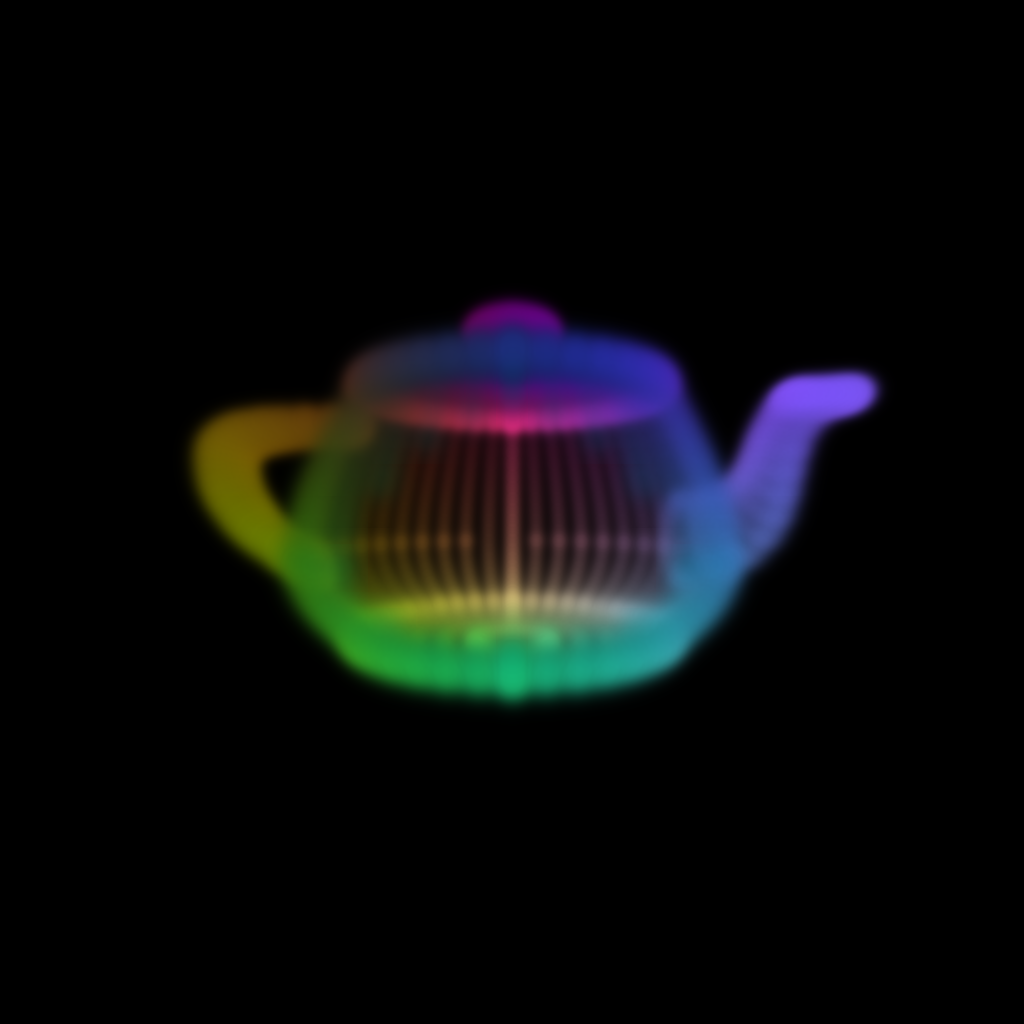
\includegraphics[scale=.2]{images/teapot.png}
        \caption{Newell Teapot rendered using renderer from Section~\ref{sec:renderer}}
        \label{fig:teapot_render}
    \end{figure}
    
    \subsection{Dense Cube}
    \label{sec:dense_cube}
    To measure the runtime improvements of the optimizations described in Chapter~\ref{ch:optimizations} I took the average
    frame time, over 500 frames, rendering a cube (see Figure~\ref{fig:cube_render}). The cube's surface consists of
    386 Gaussians. I performed this benchmark for the multithreaded rendering modes and compared them against a purely
    sequential baseline measurement.

    \begin{figure}[t]
        \centering
        
\includegraphics[scale=.2]{images/cube.png}
        \caption{Dense cube rendered using renderer from Section~\ref{sec:renderer}}
        \label{fig:cube_render}
    \end{figure}
    
    \chapter{Results and Discussion}

    The results of the experiments discussed in Chapter~\ref{ch:experiments} show that parallelized computation with
    respect to the pixels performs the best (\ref{sec:res_full_render}) and that the approximation of the error function
    by \citeauthor{AbraSteg72} and approximation of the exponential function from the VCL are best suited to the purpose
    of \gls{simd} parallelized gaussian ray tracing (\ref{sec:res_approx}).

    \section{Approximations}
    \label{sec:res_approx}
    %@TODO: Update stats on speedup & cycles per value
    The results of the approximation benchmarks show that the optimal approximations to use, in terms of speed and
    accuracy, are the approximation of the exponential function from the VCL (Vector Class Library) and the polynomial
    approximation of the error function given by \citeauthor{AbraSteg72} in the \enquote{\citetitle{AbraSteg72}}.

    The approximation of the error function in Intel's SVML is the slowest of the considered approximations. This is
    surprising because, the approximations using splines are ill-suited to the type of parallelism \gls{simd} provides.
    This is because the \gls{simd} version of the spline always needs to consider all possible cases or incur some overhead
    to determine when to return early. The sequential nature of the approximation reduce the possible gains from \gls{simd}
    parallelism.

    The polynomial approximation of the error function by \citeauthor{AbraSteg72} is both the fastest overall (see
    Figure~\ref{fig:cycles_erf}), at $\sim0.73$ cycles per value, and has the largest speedup with respect to the
    \gls{simd} version at $\sim15.3$ times faster than the sequential version (see Table~\ref{tab:abs_cycles_and_speedups_erf}).

    The Taylor approximation's maximum relative error is smaller than that of the approximation by \citeauthor{AbraSteg72}
    (see Figure~\ref{fig:erf_errors}), but its errors appear at the borders to the constant parts of the function and
    are bigger in absolute terms (see Figure~\ref{fig:erf_approx}). It is also worth noting, that the error of the
    approximation by \citeauthor{AbraSteg72} happen close to zero where small errors appear larger, due to the small
    size of the arguments.

    That the usage of splines as approximations in \gls{simd} implementations does not work well becomes more apparent,
    when looking at the performance of the spline used to approximate the exponential function. On average, it takes $6.04$
    cycles to calculate a single value of the exponential function using the spline. This is only about $3.14$ times faster
    than its sequential counterpart, as seen in Figure~\ref{fig:cycles_exp} and Table~\ref{tab:abs_cycles_and_speedups_exp}.

    Other approximations like the \enquote{Fast Exponential Function} (\ref{sec:impl_fast_exp}) or the exponential
    approximation from the VCL take as little as $0.70$ cycles per value (see Table~\ref{tab:abs_cycles_and_speedups_exp}).
    While the VCL implementation, at $0.91$ cycles per value, is slightly slower than the \enquote{Fast Exponential Function}
    it is much more accurate as seen in Figure~\ref{fig:exp_errors}. Therefore, it is the better choice overall.

    \section{Full Render}
    \label{sec:res_full_render}
    The experiments for the full render show that the tiled parallelization over the pixels performs the best overall
    regardless of the chosen compiler (\ref{sec:res_runtimes}) and that most opportunities for further optimization
    with respect to the \gls{simd} usage arise in the implementation of the transmittance function (\ref{sec:res_waste}).

    \subsection{Runtimes}
    \label{sec:res_runtimes}

    \begin{itemize}
        \item GCC (14.2.1) better at sequential and innermost loop SIMD, transmittance and radiance on par
        \item Clang (18.1.8) Mode 8 fastest overall. beats gcc in modes 7 and 8
    \end{itemize}
    \begin{figure}[t]
        \centering
        % Recommended preamble:
% \usetikzlibrary{arrows.meta}
% \usetikzlibrary{backgrounds}
% \usepgfplotslibrary{patchplots}
% \usepgfplotslibrary{fillbetween}
% \pgfplotsset{%
%     layers/standard/.define layer set={%
%         background,axis background,axis grid,axis ticks,axis lines,axis tick labels,pre main,main,axis descriptions,axis foreground%
%     }{
%         grid style={/pgfplots/on layer=axis grid},%
%         tick style={/pgfplots/on layer=axis ticks},%
%         axis line style={/pgfplots/on layer=axis lines},%
%         label style={/pgfplots/on layer=axis descriptions},%
%         legend style={/pgfplots/on layer=axis descriptions},%
%         title style={/pgfplots/on layer=axis descriptions},%
%         colorbar style={/pgfplots/on layer=axis descriptions},%
%         ticklabel style={/pgfplots/on layer=axis tick labels},%
%         axis background@ style={/pgfplots/on layer=axis background},%
%         3d box foreground style={/pgfplots/on layer=axis foreground},%
%     },
% }

\begin{tikzpicture}[/tikz/background rectangle/.style={fill={rgb,1:red,1.0;green,1.0;blue,1.0}, fill opacity={1.0}, draw opacity={1.0}}, show background rectangle, trim axis left]
\begin{axis}[point meta max={nan}, point meta min={nan}, legend cell align={left}, legend columns={1}, title={}, title style={at={{(0.5,1)}}, anchor={south}, font={{\fontsize{14 pt}{18.2 pt}\selectfont}}, color={rgb,1:red,0.0;green,0.0;blue,0.0}, draw opacity={1.0}, rotate={0.0}, align={center}}, legend style={color={rgb,1:red,0.0;green,0.0;blue,0.0}, draw opacity={1.0}, line width={1}, solid, fill={rgb,1:red,1.0;green,1.0;blue,1.0}, fill opacity={1.0}, text opacity={1.0}, font={{\fontsize{8 pt}{10.4 pt}\selectfont}}, text={rgb,1:red,0.0;green,0.0;blue,0.0}, cells={anchor={center}}, at={(0.02, 0.98)}, anchor={north west}}, axis background/.style={fill={rgb,1:red,1.0;green,1.0;blue,1.0}, opacity={1.0}}, anchor={north west}, xshift={1.0mm}, yshift={-1.0mm}, width=\textwidth, height=0.65*\textwidth, scaled x ticks={false}, xlabel={mode}, x tick style={color={rgb,1:red,0.0;green,0.0;blue,0.0}, opacity={1.0}}, x tick label style={color={rgb,1:red,0.0;green,0.0;blue,0.0}, opacity={1.0}, rotate={0}}, xlabel style={at={(ticklabel cs:0.5)}, anchor=near ticklabel, at={{(ticklabel cs:0.5)}}, anchor={near ticklabel}, font={{\fontsize{11 pt}{14.3 pt}\selectfont}}, color={rgb,1:red,0.0;green,0.0;blue,0.0}, draw opacity={1.0}, rotate={0.0}}, xmajorgrids={true}, xmin={0.4099999999999999}, xmax={3.59}, xticklabels={{seq,tr,rad,px}}, xtick={{0.5,1.5,2.5,3.5}}, xtick align={inside}, xticklabel style={font={{\fontsize{8 pt}{10.4 pt}\selectfont}}, color={rgb,1:red,0.0;green,0.0;blue,0.0}, draw opacity={1.0}, rotate={0.0}}, x grid style={color={rgb,1:red,0.0;green,0.0;blue,0.0}, draw opacity={0.1}, line width={0.5}, solid}, axis x line*={left}, x axis line style={color={rgb,1:red,0.0;green,0.0;blue,0.0}, draw opacity={1.0}, line width={1}, solid}, scaled y ticks={false}, ylabel={speedup}, y tick style={color={rgb,1:red,0.0;green,0.0;blue,0.0}, opacity={1.0}}, y tick label style={color={rgb,1:red,0.0;green,0.0;blue,0.0}, opacity={1.0}, rotate={0}}, ylabel style={at={(ticklabel cs:0.5)}, anchor=near ticklabel, at={{(ticklabel cs:0.5)}}, anchor={near ticklabel}, font={{\fontsize{11 pt}{14.3 pt}\selectfont}}, color={rgb,1:red,0.0;green,0.0;blue,0.0}, draw opacity={1.0}, rotate={0.0}}, ymajorgrids={true}, ymin={0.5192937743134411}, ymax={17.504247081905163}, yticklabels={{$3$,$6$,$9$,$12$,$15$}}, ytick={{3.0,6.0,9.0,12.0,15.0}}, ytick align={inside}, yticklabel style={font={{\fontsize{8 pt}{10.4 pt}\selectfont}}, color={rgb,1:red,0.0;green,0.0;blue,0.0}, draw opacity={1.0}, rotate={0.0}}, y grid style={color={rgb,1:red,0.0;green,0.0;blue,0.0}, draw opacity={0.1}, line width={0.5}, solid}, axis y line*={left}, y axis line style={color={rgb,1:red,0.0;green,0.0;blue,0.0}, draw opacity={1.0}, line width={1}, solid}, colorbar={false}]
    \addplot[color={rgb,1:red,0.0;green,0.6056;blue,0.9787}, name path={b81ed8e9-107d-4c5f-869b-e43c7b43cb5a}, draw opacity={1.0}, line width={1}, solid, mark={*}, mark size={3.0 pt}, mark repeat={1}, mark options={color={rgb,1:red,0.0;green,0.0;blue,0.0}, draw opacity={0.0}, fill={rgb,1:red,0.0;green,0.6056;blue,0.9787}, fill opacity={1.0}, line width={0.0}, rotate={0}, solid}]
        table[row sep={\\}]
        {
            \\
            0.5  1.034100687208785  \\
            1.5  14.719055548454257  \\
            2.5  14.676130779687545  \\
            3.5  15.085635126566041  \\
        }
        ;
    \addlegendentry {GCC v14.2.1}
    \addplot[color={rgb,1:red,0.8889;green,0.4356;blue,0.2781}, name path={0590a1cd-0581-4d69-8ce5-4881faec2f51}, draw opacity={1.0}, line width={1}, solid, mark={*}, mark size={3.0 pt}, mark repeat={1}, mark options={color={rgb,1:red,0.0;green,0.0;blue,0.0}, draw opacity={0.0}, fill={rgb,1:red,0.8889;green,0.4356;blue,0.2781}, fill opacity={1.0}, line width={0.0}, rotate={0}, solid}]
        table[row sep={\\}]
        {
            \\
            0.5  1.0  \\
            1.5  12.421015904041399  \\
            2.5  16.472729705561758  \\
            3.5  17.023540856218602  \\
        }
        ;
    \addlegendentry {Clang v18.1.8}
\end{axis}
\end{tikzpicture}

        \caption{Speedups of parallelizations relative to the slowest sequential baseline.}
        \label{fig:speedups}
    \end{figure}

    \subsection{Waste and Efficiency}
    \label{sec:res_waste}
    To make meaningful statements about the efficiency and waste of the \gls{simd} implementation it is important to know
    the \gls{throughput} and \gls{latency} statistics of the involved instructions. These can be derived from the number
    of ports that support the instruction, but it is more accurate to use measurements. I will use the measurements
    provided at \href{https://uops.info/table.html?search=&cb_lat=on&cb_tp=on&cb_uops=on&cb_ports=on&cb_ZEN4=on&cb_measurements=on&cb_doc=on&cb_avx512=on&checkbox=on}{uops.info}
    \footnote{https://uops.info/table.html?search=\&cb\_lat=on\&cb\_tp=on\&cb\_uops=on\&cb\_ports=on\&\\cb\_ZEN4=on\&cb\_measurements=on\&cb\_doc=on\&cb\_avx512=on\&checkbox=on}
    \cite{Abel19a}.

    The waste and efficiency metrics described in Section~\ref{sec:hpctoolkit} both rely on the peak number of instructions
    per cycle. What the theoretical peak actually is depends on the involved instructions and how their results depend
    on each other. I chose one instruction per cycle as the peak to work with, because most of the instructions
    involved, \eg \mintinline{s}{vaddps}, \mintinline{s}{vmulps} or \mintinline{s}{vfmadd213ps}, have a measured
    \gls{throughput} of one. Meaning that, even when ignoring all dependencies, only one instruction can be executed per
    cycle.

    %@TODO: rerun experiments with more frames to get more nuanced data

    \begin{itemize}
        \item max efficiency $47.5\%$ for radiance and $57.4\%$ for transmittance
        \item exp efficiency at $65\%$ in modes  7 and 8 instead of $33\%$ in mode 6
        \item big efficiency step with SIMD introduction small step with removal of loads
    \end{itemize}

    \chapter{Conclusion and Future Work}
    %@TODO: Short recap + what can still be done: anisotropic Gaussians, loading models learned via Gaussian splatting, more efficient tiling method using SIMD, performance left on the table TBD (see results)
    \section{Conclusion}
    \begin{itemize}
        \item SIMD + Tiling lead to massive performance improvements
    \end{itemize}

    \section{Future Work}
    There are various ways to further improve the performance and functionality of the rendering method described above.
    \begin{itemize}
        \item Memory/Cache Bottleneck? - slight data cache bottleneck in parallel versions
        \item Anisotropic Gaussians
        \item Loading Scenes learned via Gaussian splatting
        \item More efficient tiling (SIMD, Threads)
        \item Combining Splatting and Ray Tracing
        \item GPU Implementation
    \end{itemize}

    \appendix
    \chapter{Tables}
    \label{ch:tables}
    \begin{table}[b]
        \centering
        \rowcolors{1}{white}{lightgray}
        \begin{tabular}{|c | c | c | c|}
            \hline
            Mode & GCC (v14.2.1)     & Clang (v18.1.8)\\\hline
            5 mt & $\sim20.50$ sec   & $\sim21.20$ sec \\
            6 mt & $\sim1.44$ sec    & $\sim1.71$ sec \\
            7 mt & $\sim1.44$ sec    & $\sim1.29$ sec \\
            8 mt & $\sim1.40$ sec    & $\sim1.24$ sec \\
            \hline
        \end{tabular}
        \caption{Runtime of rendering the dense cube based on compiler and mode using AVX512. Averaged over 1000 Frames.}
        \label{tab:perf_dense_cube_avx512}
    \end{table}

    \begin{table}[b]
        \centering
        \rowcolors{1}{white}{lightgray}
        \begin{tabular}{|c|c|c|c|}
            \hline
            Approximation & Sequential & \gls{simd} & Speedup\\\hline
            SVML/STD & $44.90$ & $3.78$ & $11.87$\\
            Spline & $16.95$ & $3.40$ & $4.99$\\
            Spline Mirror & $13.69$ & $2.01$ & $6.81$\\
            Taylor & $12.41$ & $1.16$ & $10.68$\\
            Abramowitz and Stegun & $11.21$ & $0.73$ & $15.29$\\
            \hline
        \end{tabular}
        \caption{Average cycles per value and speedup with respect to \gls{simd} for the approximations of the error function.}
        \label{tab:abs_cycles_and_speedups_erf}
    \end{table}

    \begin{table}[b]
        \centering
        \rowcolors{1}{white}{lightgray}
        \begin{tabular}{|c|c|c|c|}
            \hline
            Approximation & Sequential & \gls{simd} & Speedup\\\hline
            SVML/STD & $11.16$ & $1.15$ & $9.68$\\
            Spline & $18.99$ & $6.04$ & $3.14$\\
            Fast Exp & $9.55$ & $0.70$ & $13.65$\\
            VCL & - & $0.91$ & -\\
            \hline
        \end{tabular}
        \caption{Average cycles per value and speedup with respect to \gls{simd} for the approximations of the exponential function.}
        \label{tab:abs_cycles_and_speedups_exp}
    \end{table}

    \begin{table}[b]
        \centering
        \rowcolors{1}{white}{lightgray}
        \begin{tabular}{|c|c|c|}
            \hline
            Function                        & Waste (\%)                       & Efficiency\\\hline
            \mintinline{c++}{radiance}      & $3.09 \cdot 10^{10}$ ($98.64\%$) & $1.36\%$\\
            \mintinline{c++}{transmittance} & $3.21 \cdot 10^{13}$ ($94.10\%$) & $5.90\%$ \\
            \hline
        \end{tabular}
        \caption{Mode 5 MT(32) Waste and Efficiency using \mintinline{c}{erff} and \mintinline{c}{expf}}
        \label{tab:mode_5_mt_wae}
    \end{table}

    \begin{table}[b]
        \centering
        \rowcolors{1}{white}{lightgray}
        \begin{tabular}{|c|c|c|}
            \hline
            Function                        & icmr     & dcmr\\\hline
            \mintinline{c++}{radiance}      & $0.16\%$ & $2.90\%$\\
            \mintinline{c++}{transmittance} & $0.02\%$ & $0.90\%$ \\
            \hline
        \end{tabular}
        \caption{Mode 5 MT(32) Instruction and Data Cache Miss Rates}
        \label{tab:mode_5_mt_cmr}
    \end{table}

    \begin{table}[b]
        \centering
        \rowcolors{1}{white}{lightgray}
        \begin{tabular}{|c|c|c|}
            \hline
            Function                                     & Waste (\%)                       & Efficiency\\\hline
            \mintinline{c++}{radiance}                   & $3.18 \cdot 10^{10}$ ($85.08\%$) & $14.92\%$\\
            \mintinline{c++}{simd_transmittance}         & $1.69 \cdot 10^{12}$ ($53.73\%$) & $46.27\%$\\
            \mintinline{c++}{simd_abramowitz_stegun_erf} & $5.72 \cdot 10^{11}$ ($47.54\%$) & $52.46\%$\\
            \mintinline{c++}{vcl_exp}                    & $1.14 \cdot 10^{12}$ ($66.47\%$) & $33.53\%$\\
            \hline
        \end{tabular}
        \caption{Mode 6 MT(32) Waste and Efficiency}
        \label{tab:mode_6_mt_wae}
    \end{table}

    \begin{table}[b]
        \centering
        \rowcolors{1}{white}{lightgray}
        \begin{tabular}{|c|c|c|}
            \hline
            Function                                     & icmr     & dcmr\\\hline
            \mintinline{c++}{radiance}                   & $0.52\%$ & $5.03\%$\\
            \mintinline{c++}{simd_transmittance}         & $0.13\%$ & $4.91\%$\\
            \mintinline{c++}{simd_abramowitz_stegun_erf} & $0.14\%$ & $3.40\%$\\
            \mintinline{c++}{vcl_exp}                    & $0.21\%$ & $5.56\%$\\
            \hline
        \end{tabular}
        \caption{Mode 6 MT(32) Instruction and Data Cache Miss Rates}
        \label{tab:mode_6_mt_cmr}
    \end{table}

    \begin{table}[b]
        \centering
        \rowcolors{1}{white}{lightgray}
        \begin{tabular}{|c|c|c|}
            \hline
            Function                                     & Waste (\%)                       & Efficiency\\\hline
            \mintinline{c++}{simd_radiance}              & $1.66 \cdot 10^{9}$ ($57.60\%$) & $42.40\%$\\
            \mintinline{c++}{broadcast_transmittance}    & $7.96 \cdot 10^{11}$ ($42.60\%$) & $57.40\%$\\
            \mintinline{c++}{simd_abramowitz_stegun_erf} & $8.20 \cdot 10^{11}$ ($40.24\%$) & $59.76\%$\\
            \mintinline{c++}{vcl_exp}                    & $4.56 \cdot 10^{11}$ ($34.29\%$) & $65.71\%$\\
            \hline
        \end{tabular}
        \caption{Mode 7 MT(32) Waste and Efficiency}
        \label{tab:mode_7_mt_wae}
    \end{table}

    \begin{table}[b]
        \centering
        \rowcolors{1}{white}{lightgray}
        \begin{tabular}{|c|c|c|}
            \hline
            Function                                     & icmr     & dcmr\\\hline
            \mintinline{c++}{simd_radiance}              & $0.02\%$ & $22.57\%$\\
            \mintinline{c++}{broadcast_transmittance}    & $0.25\%$ & $0.93\%$\\
            \mintinline{c++}{simd_abramowitz_stegun_erf} & $0.15\%$ & $0.35\%$\\
            \mintinline{c++}{vcl_exp}                    & $0.07\%$ & $0.43\%$\\
            \hline
        \end{tabular}
        \caption{Mode 7 MT(32) Instruction and Data Cache Miss Rates}
        \label{tab:mode_7_mt_cmr}
    \end{table}

    \begin{table}[b]
        \centering
        \rowcolors{1}{white}{lightgray}
        \begin{tabular}{|c|c|c|}
            \hline
            Function                                     & Waste (\%)                       & Efficiency\\\hline
            \mintinline{c++}{broadcast_radiance}         & $1.34 \cdot 10^{9}$ ($52.50\%$)  & $47.50\%$\\
            \mintinline{c++}{broadcast_transmittance}    & $7.91 \cdot 10^{11}$ ($43.01\%$) & $56.99\%$\\
            \mintinline{c++}{simd_abramowitz_stegun_erf} & $8.11 \cdot 10^{11}$ ($40.09\%$) & $59.91\%$\\
            \mintinline{c++}{vcl_exp}                    & $4.78 \cdot 10^{11}$ ($34.91\%$) & $65.09\%$\\
            \hline
        \end{tabular}
        \caption{Mode 8 MT(32) Waste and Efficiency}
        \label{tab:mode_8_mt_wae}
    \end{table}

    \begin{table}[b]
        \centering
        \rowcolors{1}{white}{lightgray}
        \begin{tabular}{|c|c|c|}
            \hline
            Function                                     & icmr     & dcmr\\\hline
            \mintinline{c++}{broadcast_radiance}         & $0.06\%$ & $11.00\%$\\
            \mintinline{c++}{broadcast_transmittance}    & $0.20\%$ & $0.91\%$\\
            \mintinline{c++}{simd_abramowitz_stegun_erf} & $0.13\%$ & $0.34\%$\\
            \mintinline{c++}{vcl_exp}                    & $0.04\%$ & $0.43\%$\\
            \hline
        \end{tabular}
        \caption{Mode 8 MT(32) Instruction and Data Cache Miss Rates}
        \label{tab:mode_8_mt_cmr}
    \end{table}

    \chapter{Figures}

    \begin{figure}
        \centering
        % Recommended preamble:
% \usetikzlibrary{arrows.meta}
% \usetikzlibrary{backgrounds}
% \usepgfplotslibrary{patchplots}
% \usepgfplotslibrary{fillbetween}
% \pgfplotsset{%
%     layers/standard/.define layer set={%
%         background,axis background,axis grid,axis ticks,axis lines,axis tick labels,pre main,main,axis descriptions,axis foreground%
%     }{
%         grid style={/pgfplots/on layer=axis grid},%
%         tick style={/pgfplots/on layer=axis ticks},%
%         axis line style={/pgfplots/on layer=axis lines},%
%         label style={/pgfplots/on layer=axis descriptions},%
%         legend style={/pgfplots/on layer=axis descriptions},%
%         title style={/pgfplots/on layer=axis descriptions},%
%         colorbar style={/pgfplots/on layer=axis descriptions},%
%         ticklabel style={/pgfplots/on layer=axis tick labels},%
%         axis background@ style={/pgfplots/on layer=axis background},%
%         3d box foreground style={/pgfplots/on layer=axis foreground},%
%     },
% }

\begin{tikzpicture}[/tikz/background rectangle/.style={fill={rgb,1:red,1.0;green,1.0;blue,1.0}, fill opacity={1.0}, draw opacity={1.0}}, show background rectangle]
\begin{axis}[point meta max={nan}, point meta min={nan}, legend cell align={left}, legend columns={1}, title={}, title style={at={{(0.5,1)}}, anchor={south}, font={{\fontsize{14 pt}{18.2 pt}\selectfont}}, color={rgb,1:red,0.0;green,0.0;blue,0.0}, draw opacity={1.0}, rotate={0.0}, align={center}}, legend style={color={rgb,1:red,0.0;green,0.0;blue,0.0}, draw opacity={1.0}, line width={1}, solid, fill={rgb,1:red,1.0;green,1.0;blue,1.0}, fill opacity={1.0}, text opacity={1.0}, font={{\fontsize{8 pt}{10.4 pt}\selectfont}}, text={rgb,1:red,0.0;green,0.0;blue,0.0}, cells={anchor={center}}, at={(0.02, 0.98)}, anchor={north west}}, axis background/.style={fill={rgb,1:red,1.0;green,1.0;blue,1.0}, opacity={1.0}}, anchor={north west}, xshift={1.0mm}, yshift={-1.0mm}, width={150.4mm}, height={99.6mm}, scaled x ticks={false}, xlabel={}, x tick style={color={rgb,1:red,0.0;green,0.0;blue,0.0}, opacity={1.0}}, x tick label style={color={rgb,1:red,0.0;green,0.0;blue,0.0}, opacity={1.0}, rotate={0}}, xlabel style={at={(ticklabel cs:0.5)}, anchor=near ticklabel, at={{(ticklabel cs:0.5)}}, anchor={near ticklabel}, font={{\fontsize{11 pt}{14.3 pt}\selectfont}}, color={rgb,1:red,0.0;green,0.0;blue,0.0}, draw opacity={1.0}, rotate={0.0}}, xmajorgrids={true}, xmin={-0.18392000000000008}, xmax={5.1839200000000005}, xticklabels={{Abramowitz,SVML/STD,Spline,Spline Mirror,Taylor}}, xtick={{0.5,1.5,2.5,3.5,4.5}}, xtick align={inside}, xticklabel style={font={{\fontsize{8 pt}{10.4 pt}\selectfont}}, color={rgb,1:red,0.0;green,0.0;blue,0.0}, draw opacity={1.0}, rotate={0.0}}, x grid style={color={rgb,1:red,0.0;green,0.0;blue,0.0}, draw opacity={0.1}, line width={0.5}, solid}, axis x line*={left}, x axis line style={color={rgb,1:red,0.0;green,0.0;blue,0.0}, draw opacity={1.0}, line width={1}, solid}, scaled y ticks={false}, ylabel={avg. cycles}, y tick style={color={rgb,1:red,0.0;green,0.0;blue,0.0}, opacity={1.0}}, y tick label style={color={rgb,1:red,0.0;green,0.0;blue,0.0}, opacity={1.0}, rotate={0}}, ylabel style={at={(ticklabel cs:0.5)}, anchor=near ticklabel, at={{(ticklabel cs:0.5)}}, anchor={near ticklabel}, font={{\fontsize{11 pt}{14.3 pt}\selectfont}}, color={rgb,1:red,0.0;green,0.0;blue,0.0}, draw opacity={1.0}, rotate={0.0}}, ymajorgrids={true}, ymin={0.0}, ymax={61.355656}, yticklabels={{$0$,$10$,$20$,$30$,$40$,$50$,$60$}}, ytick={{0.0,10.0,20.0,30.0,40.0,50.0,60.0}}, ytick align={inside}, yticklabel style={font={{\fontsize{8 pt}{10.4 pt}\selectfont}}, color={rgb,1:red,0.0;green,0.0;blue,0.0}, draw opacity={1.0}, rotate={0.0}}, y grid style={color={rgb,1:red,0.0;green,0.0;blue,0.0}, draw opacity={0.1}, line width={0.5}, solid}, axis y line*={left}, y axis line style={color={rgb,1:red,0.0;green,0.0;blue,0.0}, draw opacity={1.0}, line width={1}, solid}, colorbar={false}]
    \addplot[color={rgb,1:red,0.0;green,0.0;blue,0.0}, name path={1}, area legend, fill={rgb,1:red,0.0;green,0.6056;blue,0.9787}, fill opacity={1.0}, draw opacity={1.0}, line width={1}, solid]
        table[row sep={\\}]
        {
            \\
            0.09999999999999998  2.495022  \\
            0.09999999999999998  0.0  \\
            0.5  0.0  \\
            0.5  2.495022  \\
            0.09999999999999998  2.495022  \\
        }
        ;
    \addlegendentry {SIMD}
    \addplot[color={rgb,1:red,0.0;green,0.0;blue,0.0}, name path={1}, area legend, fill={rgb,1:red,0.0;green,0.6056;blue,0.9787}, fill opacity={1.0}, draw opacity={1.0}, line width={1}, solid, forget plot]
        table[row sep={\\}]
        {
            \\
            1.1  5.6820583  \\
            1.1  0.0  \\
            1.5  0.0  \\
            1.5  5.6820583  \\
            1.1  5.6820583  \\
        }
        ;
    \addplot[color={rgb,1:red,0.0;green,0.0;blue,0.0}, name path={1}, area legend, fill={rgb,1:red,0.0;green,0.6056;blue,0.9787}, fill opacity={1.0}, draw opacity={1.0}, line width={1}, solid, forget plot]
        table[row sep={\\}]
        {
            \\
            2.1  4.1816087  \\
            2.1  0.0  \\
            2.5000000000000004  0.0  \\
            2.5000000000000004  4.1816087  \\
            2.1  4.1816087  \\
        }
        ;
    \addplot[color={rgb,1:red,0.0;green,0.0;blue,0.0}, name path={1}, area legend, fill={rgb,1:red,0.0;green,0.6056;blue,0.9787}, fill opacity={1.0}, draw opacity={1.0}, line width={1}, solid, forget plot]
        table[row sep={\\}]
        {
            \\
            3.1  3.3629444  \\
            3.1  0.0  \\
            3.5000000000000004  0.0  \\
            3.5000000000000004  3.3629444  \\
            3.1  3.3629444  \\
        }
        ;
    \addplot[color={rgb,1:red,0.0;green,0.0;blue,0.0}, name path={1}, area legend, fill={rgb,1:red,0.0;green,0.6056;blue,0.9787}, fill opacity={1.0}, draw opacity={1.0}, line width={1}, solid, forget plot]
        table[row sep={\\}]
        {
            \\
            4.1  2.6012878  \\
            4.1  0.0  \\
            4.5  0.0  \\
            4.5  2.6012878  \\
            4.1  2.6012878  \\
        }
        ;
    \addplot[color={rgb,1:red,0.0;green,0.6056;blue,0.9787}, name path={2}, only marks, draw opacity={1.0}, line width={0}, solid, mark={*}, mark size={0.0 pt}, mark repeat={1}, mark options={color={rgb,1:red,0.0;green,0.0;blue,0.0}, draw opacity={0.0}, fill={rgb,1:red,0.0;green,0.6056;blue,0.9787}, fill opacity={0.0}, line width={0.75}, rotate={0}, solid}, forget plot]
        table[row sep={\\}]
        {
            \\
            0.3  2.495022  \\
            1.3  5.6820583  \\
            2.3000000000000003  4.1816087  \\
            3.3000000000000003  3.3629444  \\
            4.3  2.6012878  \\
        }
        ;
    \addplot[color={rgb,1:red,0.0;green,0.0;blue,0.0}, name path={3}, area legend, fill={rgb,1:red,0.8889;green,0.4356;blue,0.2781}, fill opacity={1.0}, draw opacity={1.0}, line width={1}, solid]
        table[row sep={\\}]
        {
            \\
            0.49999999999999994  12.119275  \\
            0.49999999999999994  0.0  \\
            0.8999999999999999  0.0  \\
            0.8999999999999999  12.119275  \\
            0.49999999999999994  12.119275  \\
        }
        ;
    \addlegendentry {Sequential}
    \addplot[color={rgb,1:red,0.0;green,0.0;blue,0.0}, name path={3}, area legend, fill={rgb,1:red,0.8889;green,0.4356;blue,0.2781}, fill opacity={1.0}, draw opacity={1.0}, line width={1}, solid, forget plot]
        table[row sep={\\}]
        {
            \\
            1.5000000000000002  61.355656  \\
            1.5000000000000002  0.0  \\
            1.9000000000000001  0.0  \\
            1.9000000000000001  61.355656  \\
            1.5000000000000002  61.355656  \\
        }
        ;
    \addplot[color={rgb,1:red,0.0;green,0.0;blue,0.0}, name path={3}, area legend, fill={rgb,1:red,0.8889;green,0.4356;blue,0.2781}, fill opacity={1.0}, draw opacity={1.0}, line width={1}, solid, forget plot]
        table[row sep={\\}]
        {
            \\
            2.5  39.78879  \\
            2.5  0.0  \\
            2.9000000000000004  0.0  \\
            2.9000000000000004  39.78879  \\
            2.5  39.78879  \\
        }
        ;
    \addplot[color={rgb,1:red,0.0;green,0.0;blue,0.0}, name path={3}, area legend, fill={rgb,1:red,0.8889;green,0.4356;blue,0.2781}, fill opacity={1.0}, draw opacity={1.0}, line width={1}, solid, forget plot]
        table[row sep={\\}]
        {
            \\
            3.5  48.166466  \\
            3.5  0.0  \\
            3.9000000000000004  0.0  \\
            3.9000000000000004  48.166466  \\
            3.5  48.166466  \\
        }
        ;
    \addplot[color={rgb,1:red,0.0;green,0.0;blue,0.0}, name path={3}, area legend, fill={rgb,1:red,0.8889;green,0.4356;blue,0.2781}, fill opacity={1.0}, draw opacity={1.0}, line width={1}, solid, forget plot]
        table[row sep={\\}]
        {
            \\
            4.5  30.905552  \\
            4.5  0.0  \\
            4.9  0.0  \\
            4.9  30.905552  \\
            4.5  30.905552  \\
        }
        ;
    \addplot[color={rgb,1:red,0.8889;green,0.4356;blue,0.2781}, name path={4}, only marks, draw opacity={1.0}, line width={0}, solid, mark={*}, mark size={0.0 pt}, mark repeat={1}, mark options={color={rgb,1:red,0.0;green,0.0;blue,0.0}, draw opacity={0.0}, fill={rgb,1:red,0.8889;green,0.4356;blue,0.2781}, fill opacity={0.0}, line width={0.75}, rotate={0}, solid}, forget plot]
        table[row sep={\\}]
        {
            \\
            0.7  12.119275  \\
            1.7000000000000002  61.355656  \\
            2.7  39.78879  \\
            3.7  48.166466  \\
            4.7  30.905552  \\
        }
        ;
\end{axis}
\end{tikzpicture}

        \caption{Average cycle count to calculate one value of $\erf$.}
        \label{fig:cycles_erf}
    \end{figure}

    \begin{figure}
        \centering
        % Recommended preamble:
% \usetikzlibrary{arrows.meta}
% \usetikzlibrary{backgrounds}
% \usepgfplotslibrary{patchplots}
% \usepgfplotslibrary{fillbetween}
% \pgfplotsset{%
%     layers/standard/.define layer set={%
%         background,axis background,axis grid,axis ticks,axis lines,axis tick labels,pre main,main,axis descriptions,axis foreground%
%     }{
%         grid style={/pgfplots/on layer=axis grid},%
%         tick style={/pgfplots/on layer=axis ticks},%
%         axis line style={/pgfplots/on layer=axis lines},%
%         label style={/pgfplots/on layer=axis descriptions},%
%         legend style={/pgfplots/on layer=axis descriptions},%
%         title style={/pgfplots/on layer=axis descriptions},%
%         colorbar style={/pgfplots/on layer=axis descriptions},%
%         ticklabel style={/pgfplots/on layer=axis tick labels},%
%         axis background@ style={/pgfplots/on layer=axis background},%
%         3d box foreground style={/pgfplots/on layer=axis foreground},%
%     },
% }

\begin{tikzpicture}[/tikz/background rectangle/.style={fill={rgb,1:red,1.0;green,1.0;blue,1.0}, fill opacity={1.0}, draw opacity={1.0}}, show background rectangle, trim axis left]
\begin{axis}[point meta max={nan}, point meta min={nan}, legend cell align={left}, legend columns={1}, title={}, title style={at={{(0.5,1)}}, anchor={south}, font={{\fontsize{14 pt}{18.2 pt}\selectfont}}, color={rgb,1:red,0.0;green,0.0;blue,0.0}, draw opacity={1.0}, rotate={0.0}, align={center}}, legend style={color={rgb,1:red,0.0;green,0.0;blue,0.0}, draw opacity={1.0}, line width={1}, solid, fill={rgb,1:red,1.0;green,1.0;blue,1.0}, fill opacity={1.0}, text opacity={1.0}, font={{\fontsize{8 pt}{10.4 pt}\selectfont}}, text={rgb,1:red,0.0;green,0.0;blue,0.0}, cells={anchor={center}}, at={(0.02, 0.98)}, anchor={north west}}, axis background/.style={fill={rgb,1:red,1.0;green,1.0;blue,1.0}, opacity={1.0}}, anchor={north west}, xshift={1.0mm}, yshift={-1.0mm}, width=\textwidth, height=0.65*\textwidth, scaled x ticks={false}, xlabel={$x$}, x tick style={color={rgb,1:red,0.0;green,0.0;blue,0.0}, opacity={1.0}}, x tick label style={color={rgb,1:red,0.0;green,0.0;blue,0.0}, opacity={1.0}, rotate={0}}, xlabel style={at={(ticklabel cs:0.5)}, anchor=near ticklabel, at={{(ticklabel cs:0.5)}}, anchor={near ticklabel}, font={{\fontsize{11 pt}{14.3 pt}\selectfont}}, color={rgb,1:red,0.0;green,0.0;blue,0.0}, draw opacity={1.0}, rotate={0.0}}, xmajorgrids={true}, xmin={-6.359999799000001}, xmax={6.359993099}, xticklabels={{$-5.0$,$-2.5$,$0.0$,$2.5$,$5.0$}}, xtick={{-5.0,-2.5,0.0,2.5,5.0}}, xtick align={inside}, xticklabel style={font={{\fontsize{8 pt}{10.4 pt}\selectfont}}, color={rgb,1:red,0.0;green,0.0;blue,0.0}, draw opacity={1.0}, rotate={0.0}}, x grid style={color={rgb,1:red,0.0;green,0.0;blue,0.0}, draw opacity={0.1}, line width={0.5}, solid}, axis x line*={left}, x axis line style={color={rgb,1:red,0.0;green,0.0;blue,0.0}, draw opacity={1.0}, line width={1}, solid}, scaled y ticks={false}, ylabel={err}, y tick style={color={rgb,1:red,0.0;green,0.0;blue,0.0}, opacity={1.0}}, y tick label style={color={rgb,1:red,0.0;green,0.0;blue,0.0}, opacity={1.0}, rotate={0}}, ylabel style={at={(ticklabel cs:0.5)}, anchor=near ticklabel, at={{(ticklabel cs:0.5)}}, anchor={near ticklabel}, font={{\fontsize{11 pt}{14.3 pt}\selectfont}}, color={rgb,1:red,0.0;green,0.0;blue,0.0}, draw opacity={1.0}, rotate={0.0}}, ymajorgrids={true}, ymin={-0.0030000000000000027}, ymax={0.10300000000000001}, yticklabels={{$0.000$,$0.025$,$0.050$,$0.075$,$0.100$}}, ytick={{0.0,0.025000000000000005,0.05000000000000001,0.07500000000000001,0.10000000000000002}}, ytick align={inside}, yticklabel style={font={{\fontsize{8 pt}{10.4 pt}\selectfont}}, color={rgb,1:red,0.0;green,0.0;blue,0.0}, draw opacity={1.0}, rotate={0.0}}, y grid style={color={rgb,1:red,0.0;green,0.0;blue,0.0}, draw opacity={0.1}, line width={0.5}, solid}, axis y line*={left}, y axis line style={color={rgb,1:red,0.0;green,0.0;blue,0.0}, draw opacity={1.0}, line width={1}, solid}, colorbar={false}]
    \addplot[color={rgb,1:red,0.0;green,0.6056;blue,0.9787}, name path={b96da881-5eb9-4b2a-8fa3-a476c10391ea}, draw opacity={1.0}, line width={1}, solid]
        table[row sep={\\}]
        {
            \\
            -6.0  0.0  \\
            -5.9  0.0  \\
            -5.8  0.0  \\
            -5.7000003  0.0  \\
            -5.6000004  0.0  \\
            -5.5000005  0.0  \\
            -5.4000006  0.0  \\
            -5.3000007  0.0  \\
            -5.200001  0.0  \\
            -5.100001  0.0  \\
            -5.000001  0.0  \\
            -4.900001  0.0  \\
            -4.800001  0.0  \\
            -4.7000012  0.0  \\
            -4.6000013  0.0  \\
            -4.5000014  0.0  \\
            -4.4000015  0.0  \\
            -4.3000016  0.0  \\
            -4.2000017  0.0  \\
            -4.100002  0.0  \\
            -4.000002  0.0  \\
            -3.900002  1.53846074869753e-8  \\
            -3.800002  1.5789465365654716e-8  \\
            -3.7000022  5.405402191537917e-8  \\
            -3.6000023  9.999993612019539e-8  \\
            -3.5000024  1.999998628471277e-7  \\
            -3.4000025  4.558820177387563e-7  \\
            -3.3000026  9.212113953953219e-7  \\
            -3.2000027  1.8749984179546126e-6  \\
            -3.1000028  3.7419321040614862e-6  \\
            -3.0000029  7.366659545570731e-6  \\
            -2.900003  1.416205431510809e-5  \\
            -2.800003  3.499996250025361e-6  \\
            -2.7000031  1.368516947255525e-5  \\
            -2.6000032  3.743456931130184e-5  \\
            -2.5000033  8.663988563535545e-5  \\
            -2.4000034  0.0001812914098371784  \\
            -2.3000035  0.0003539385918326041  \\
            -2.2000036  6.888625091340773e-5  \\
            -2.1000037  0.00025085670087149776  \\
            -2.0000038  0.0006433737775898242  \\
            -1.9000038  0.001399786674110854  \\
            -1.8000038  0.0027532552986832435  \\
            -1.7000037  0.005049483127595524  \\
            -1.6000037  0.0002693743770717969  \\
            -1.5000037  0.0011188439068516842  \\
            -1.4000037  0.0030393491102916055  \\
            -1.3000036  0.006753596682347608  \\
            -1.2000036  0.013291260126219553  \\
            -1.1000036  0.024091193883365454  \\
            -1.0000036  0.0009310666481599894  \\
            -0.90000355  0.0025389899850951033  \\
            -0.8000035  0.005417276299416232  \\
            -0.7000035  0.010854288585700048  \\
            -0.6000035  0.02153820769378848  \\
            -0.50000346  0.04308260186839511  \\
            -0.40000346  0.002260730444681576  \\
            -0.30000347  0.01554325354970065  \\
            -0.20000347  0.06587725702959052  \\
            -0.10000347  0.1  \\
            -3.4719706e-6  0.1  \\
            0.09999653  0.1  \\
            0.19999653  0.007688883402127048  \\
            0.29999653  0.011675401712146581  \\
            0.39999652  0.015433834274358208  \\
            0.4999965  0.020346442425096905  \\
            0.5999965  0.027550727379243006  \\
            0.69999653  0.038153903420064174  \\
            0.79999655  0.00022750098109800034  \\
            0.8999966  0.0035040687931487827  \\
            0.9999966  0.010773136628664517  \\
            1.0999966  0.022860888842747406  \\
            1.1999966  0.04045711462849139  \\
            1.2999966  0.06410639843211903  \\
            1.3999966  0.00031682219799673746  \\
            1.4999967  0.0006569014451831767  \\
            1.5999967  0.0010497896651911669  \\
            1.6999967  0.0015797089488467874  \\
            1.7999967  0.002377059913498713  \\
            1.8999968  0.0036062744947780757  \\
            1.9999968  1.3590021744042553e-5  \\
            2.0999968  0.0003832862983410247  \\
            2.1999967  0.0012843655629120238  \\
            2.2999966  0.0028909173170081916  \\
            2.3999965  0.005369903664442834  \\
            2.4999964  0.008877572783704804  \\
            2.5999963  2.4730804424612883e-6  \\
            2.6999962  5.550007811118249e-5  \\
            2.7999961  0.00018976455002919155  \\
            2.899996  0.00043503508280704005  \\
            2.999996  0.000819434425912576  \\
            3.0999959  0.0013685824552219878  \\
            3.1999958  1.875002460925258e-6  \\
            3.2999957  9.21213321567113e-7  \\
            3.3999956  4.5588294291228366e-7  \\
            3.4999955  2.0000025713307856e-7  \\
            3.5999954  1.0000012778698454e-7  \\
            3.6999953  5.4054122718953494e-8  \\
            3.7999952  1.5789493620523163e-8  \\
            3.899995  1.5384635100408756e-8  \\
            3.999995  0.0  \\
            4.099995  0.0  \\
            4.199995  0.0  \\
            4.299995  0.0  \\
            4.399995  0.0  \\
            4.4999948  0.0  \\
            4.5999947  0.0  \\
            4.6999946  0.0  \\
            4.7999945  0.0  \\
            4.8999944  0.0  \\
            4.9999943  0.0  \\
            5.099994  0.0  \\
            5.199994  0.0  \\
            5.299994  0.0  \\
            5.399994  0.0  \\
            5.499994  0.0  \\
            5.5999937  0.0  \\
            5.6999936  0.0  \\
            5.7999935  0.0  \\
            5.8999934  0.0  \\
            5.9999933  0.0  \\
        }
        ;
    \addlegendentry {spline}
    \addplot[color={rgb,1:red,0.8889;green,0.4356;blue,0.2781}, name path={80cf943e-4445-46ea-82a1-a71334981008}, draw opacity={1.0}, line width={1}, solid]
        table[row sep={\\}]
        {
            \\
            -6.0  0.0  \\
            -5.9  0.0  \\
            -5.8  0.0  \\
            -5.7000003  0.0  \\
            -5.6000004  0.0  \\
            -5.5000005  0.0  \\
            -5.4000006  0.0  \\
            -5.3000007  0.0  \\
            -5.200001  0.0  \\
            -5.100001  0.0  \\
            -5.000001  0.0  \\
            -4.900001  0.0  \\
            -4.800001  0.0  \\
            -4.7000012  0.0  \\
            -4.6000013  0.0  \\
            -4.5000014  0.0  \\
            -4.4000015  0.0  \\
            -4.3000016  0.0  \\
            -4.2000017  0.0  \\
            -4.100002  0.0  \\
            -4.000002  0.0  \\
            -3.900002  1.53846074869753e-8  \\
            -3.800002  1.5789465365654716e-8  \\
            -3.7000022  5.405402191537917e-8  \\
            -3.6000023  9.999993612019539e-8  \\
            -3.5000024  1.999998628471277e-7  \\
            -3.4000025  4.558820177387563e-7  \\
            -3.3000026  9.212113953953219e-7  \\
            -3.2000027  1.8749984179546126e-6  \\
            -3.1000028  3.7419321040614862e-6  \\
            -3.0000029  7.366659545570731e-6  \\
            -2.900003  1.416205431510809e-5  \\
            -2.800003  3.499996250025361e-6  \\
            -2.7000031  1.368516947255525e-5  \\
            -2.6000032  3.743456931130184e-5  \\
            -2.5000033  8.663988563535545e-5  \\
            -2.4000034  0.0001812914098371784  \\
            -2.3000035  0.0003539385918326041  \\
            -2.2000036  6.888625091340773e-5  \\
            -2.1000037  0.00025085670087149776  \\
            -2.0000038  0.0006433737775898242  \\
            -1.9000038  0.001399786674110854  \\
            -1.8000038  0.0027532552986832435  \\
            -1.7000037  0.005049483127595524  \\
            -1.6000037  0.0002693743770717969  \\
            -1.5000037  0.0011188439068516842  \\
            -1.4000037  0.0030393491102916055  \\
            -1.3000036  0.006753596682347608  \\
            -1.2000036  0.013291260126219553  \\
            -1.1000036  0.024091193883365454  \\
            -1.0000036  0.0009310666481599894  \\
            -0.90000355  0.0025389899850951033  \\
            -0.8000035  0.005417276299416232  \\
            -0.7000035  0.010854288585700048  \\
            -0.6000035  0.02153820769378848  \\
            -0.50000346  0.04308260186839511  \\
            -0.40000346  0.002260730444681576  \\
            -0.30000347  0.01554325354970065  \\
            -0.20000347  0.06587725702959052  \\
            -0.10000347  0.1  \\
            -3.4719706e-6  0.1  \\
            0.09999653  0.1  \\
            0.19999653  0.06588354307947238  \\
            0.29999653  0.015544979803599791  \\
            0.39999652  0.0022610946715236713  \\
            0.4999965  0.0  \\
            0.5999965  0.021539358979594157  \\
            0.69999653  0.0108548109517057  \\
            0.79999655  0.005417598363392977  \\
            0.8999966  0.0025390651475793997  \\
            0.9999966  0.0009312031660907856  \\
            1.0999966  0.0  \\
            1.1999966  0.013291812660135877  \\
            1.2999966  0.006753979202714827  \\
            1.3999966  0.003039507381660757  \\
            1.4999967  0.0011189357949921354  \\
            1.5999967  0.0002694130556643821  \\
            1.6999967  0.0  \\
            1.7999967  0.0027533939367777836  \\
            1.8999968  0.0013998234102288764  \\
            1.9999968  0.0006434310294896476  \\
            2.0999968  0.0002508575251162523  \\
            2.1999967  6.890919427289573e-5  \\
            2.2999966  1.739133004759475e-8  \\
            2.3999965  0.00018131276441446927  \\
            2.4999964  8.668012481940758e-5  \\
            2.5999963  3.7434668657031004e-5  \\
            2.6999962  1.3685204445815346e-5  \\
            2.7999961  3.4892905743761717e-6  \\
            2.899996  0.0  \\
            2.999996  7.366676488910278e-6  \\
            3.0999959  3.7419404328891206e-6  \\
            3.1999958  1.875002460925258e-6  \\
            3.2999957  9.21213321567113e-7  \\
            3.3999956  4.5588294291228366e-7  \\
            3.4999955  2.0000025713307856e-7  \\
            3.5999954  1.0000012778698454e-7  \\
            3.6999953  5.4054122718953494e-8  \\
            3.7999952  1.5789493620523163e-8  \\
            3.899995  1.5384635100408756e-8  \\
            3.999995  0.0  \\
            4.099995  0.0  \\
            4.199995  0.0  \\
            4.299995  0.0  \\
            4.399995  0.0  \\
            4.4999948  0.0  \\
            4.5999947  0.0  \\
            4.6999946  0.0  \\
            4.7999945  0.0  \\
            4.8999944  0.0  \\
            4.9999943  0.0  \\
            5.099994  0.0  \\
            5.199994  0.0  \\
            5.299994  0.0  \\
            5.399994  0.0  \\
            5.499994  0.0  \\
            5.5999937  0.0  \\
            5.6999936  0.0  \\
            5.7999935  0.0  \\
            5.8999934  0.0  \\
            5.9999933  0.0  \\
        }
        ;
    \addlegendentry {mirror}
    \addplot[color={rgb,1:red,0.2422;green,0.6433;blue,0.3044}, name path={31622ab0-c463-462d-95af-fc0e14c02ac3}, draw opacity={1.0}, line width={1}, solid]
        table[row sep={\\}]
        {
            \\
            -6.0  0.0  \\
            -5.9  0.0  \\
            -5.8  0.0  \\
            -5.7000003  0.0  \\
            -5.6000004  0.0  \\
            -5.5000005  0.0  \\
            -5.4000006  0.0  \\
            -5.3000007  0.0  \\
            -5.200001  0.0  \\
            -5.100001  0.0  \\
            -5.000001  0.0  \\
            -4.900001  0.0  \\
            -4.800001  0.0  \\
            -4.7000012  0.0  \\
            -4.6000013  0.0  \\
            -4.5000014  0.0  \\
            -4.4000015  0.0  \\
            -4.3000016  0.0  \\
            -4.2000017  0.0  \\
            -4.100002  0.0  \\
            -4.000002  0.0  \\
            -3.900002  1.53846074869753e-8  \\
            -3.800002  1.5789465365654716e-8  \\
            -3.7000022  5.405402191537917e-8  \\
            -3.6000023  9.999993612019539e-8  \\
            -3.5000024  1.999998628471277e-7  \\
            -3.4000025  4.558820177387563e-7  \\
            -3.3000026  9.212113953953219e-7  \\
            -3.2000027  1.8749984179546126e-6  \\
            -3.1000028  3.7419321040614862e-6  \\
            -3.0000029  7.366659545570731e-6  \\
            -2.900003  1.416205431510809e-5  \\
            -2.800003  2.678568558678232e-5  \\
            -2.7000031  4.975920212830489e-5  \\
            -2.6000032  9.078065750074987e-5  \\
            -2.5000033  0.00016275978515707874  \\
            -2.4000034  0.00028687459359431775  \\
            -2.3000035  0.0004970253306136413  \\
            -2.2000036  0.0008467258871758452  \\
            -2.1000037  0.0014187594050429366  \\
            -2.0000038  0.002338820556240932  \\
            -1.9000038  0.004264465155280222  \\
            -1.8000038  0.0014822746485312704  \\
            -1.7000037  0.0004838812997877632  \\
            -1.6000037  0.00014722465954292011  \\
            -1.5000037  4.1399897880221136e-5  \\
            -1.4000037  1.059282914753812e-5  \\
            -1.3000036  2.4153779266554163e-6  \\
            -1.2000036  4.1666541672865727e-7  \\
            -1.1000036  1.1818143139448353e-7  \\
            -1.0000036  2.999989204010913e-8  \\
            -0.90000355  1.1111067278275115e-7  \\
            -0.8000035  7.499967183695903e-8  \\
            -0.7000035  8.5713857099884e-8  \\
            -0.6000035  0.0  \\
            -0.50000346  0.0  \\
            -0.40000346  4.999956747742353e-8  \\
            -0.30000347  9.999884329407698e-8  \\
            -0.20000347  0.0  \\
            -0.10000347  4.999826503388553e-8  \\
            -3.4719706e-6  0.0  \\
            0.09999653  0.0  \\
            0.19999653  1.0000173511624655e-7  \\
            0.29999653  6.666743775160628e-8  \\
            0.39999652  0.0  \\
            0.4999965  0.0  \\
            0.5999965  0.0  \\
            0.69999653  1.0000049574340926e-7  \\
            0.79999655  0.0  \\
            0.8999966  3.333345930386901e-8  \\
            0.9999966  0.0  \\
            1.0999966  5.454562321323625e-8  \\
            1.1999966  4.7500134581842395e-7  \\
            1.2999966  2.4076986048066217e-6  \\
            1.3999966  1.0621454366389291e-5  \\
            1.4999967  4.1366757673483324e-5  \\
            1.5999967  0.00014731280383269594  \\
            1.6999967  0.0004839421158876097  \\
            1.7999967  0.0014822249396346137  \\
            1.8999968  0.004264154550155034  \\
            1.9999968  0.01159715355544567  \\
            2.0999968  0.0014188116858082946  \\
            2.1999967  0.0008467739974337238  \\
            2.2999966  0.0004970442130218848  \\
            2.3999965  0.0002868962517237046  \\
            2.4999964  0.00016280023443235607  \\
            2.5999963  9.078089841899149e-5  \\
            2.6999962  4.975932929088929e-5  \\
            2.7999961  2.6800037328632777e-5  \\
            2.899996  1.4172433341292927e-5  \\
            2.999996  7.366676488910278e-6  \\
            3.0999959  3.7419404328891206e-6  \\
            3.1999958  1.875002460925258e-6  \\
            3.2999957  9.21213321567113e-7  \\
            3.3999956  4.5588294291228366e-7  \\
            3.4999955  2.0000025713307856e-7  \\
            3.5999954  1.0000012778698454e-7  \\
            3.6999953  5.4054122718953494e-8  \\
            3.7999952  1.5789493620523163e-8  \\
            3.899995  1.5384635100408756e-8  \\
            3.999995  0.0  \\
            4.099995  0.0  \\
            4.199995  0.0  \\
            4.299995  0.0  \\
            4.399995  0.0  \\
            4.4999948  0.0  \\
            4.5999947  0.0  \\
            4.6999946  0.0  \\
            4.7999945  0.0  \\
            4.8999944  0.0  \\
            4.9999943  0.0  \\
            5.099994  0.0  \\
            5.199994  0.0  \\
            5.299994  0.0  \\
            5.399994  0.0  \\
            5.499994  0.0  \\
            5.5999937  0.0  \\
            5.6999936  0.0  \\
            5.7999935  0.0  \\
            5.8999934  0.0  \\
            5.9999933  0.0  \\
        }
        ;
    \addlegendentry {taylor}
    \addplot[color={rgb,1:red,0.7644;green,0.4441;blue,0.8243}, name path={9d285fe8-c829-4112-a0f9-a222cdf1fc0d}, draw opacity={1.0}, line width={1}, solid]
        table[row sep={\\}]
        {
            \\
            -6.0  0.0  \\
            -5.9  0.0  \\
            -5.8  0.0  \\
            -5.7000003  0.0  \\
            -5.6000004  0.0  \\
            -5.5000005  0.0  \\
            -5.4000006  1.111110987069495e-8  \\
            -5.3000007  1.1320753215828566e-8  \\
            -5.200001  1.1538459313453718e-8  \\
            -5.100001  1.1764703569355898e-8  \\
            -5.000001  1.9999995989473686e-8  \\
            -4.900001  2.0408159089633742e-8  \\
            -4.800001  4.166665798731107e-8  \\
            -4.7000012  5.106381674640783e-8  \\
            -4.6000013  6.521737286315887e-8  \\
            -4.5000014  8.888886123713256e-8  \\
            -4.4000015  1.3636358987997012e-7  \\
            -4.3000016  1.9302318398014147e-7  \\
            -4.2000017  2.6904751015120794e-7  \\
            -4.100002  3.9024371208745975e-7  \\
            -4.000002  5.649997175080615e-7  \\
            -3.900002  7.948713872540658e-7  \\
            -3.800002  1.168420437671993e-6  \\
            -3.7000022  1.6864854837238227e-6  \\
            -3.6000023  2.4666650907386634e-6  \\
            -3.5000024  3.5999975314386223e-6  \\
            -3.4000025  5.220584396640464e-6  \\
            -3.3000026  7.624236417292387e-6  \\
            -3.2000027  1.1031240692412973e-5  \\
            -3.1000028  1.590321144227027e-5  \\
            -3.0000029  2.2699978056693002e-5  \\
            -2.900003  3.206203579790099e-5  \\
            -2.800003  4.4678523558720874e-5  \\
            -2.7000031  6.116659643837383e-5  \\
            -2.6000032  8.211912969950068e-5  \\
            -2.5000033  0.00010755985802099395  \\
            -2.4000034  0.00013679147287877136  \\
            -2.3000035  0.00016795626615348654  \\
            -2.2000036  0.0001975451312897632  \\
            -2.1000037  0.00022002342186349085  \\
            -2.0000038  0.0002280745666583176  \\
            -1.9000038  0.00021315746842189934  \\
            -1.8000038  0.00016755520182791447  \\
            -1.7000037  8.682334044333286e-5  \\
            -1.6000037  2.6062439730628983e-5  \\
            -1.5000037  0.0001572662787431495  \\
            -1.4000037  0.0002801921166351006  \\
            -1.3000036  0.00035741439485245744  \\
            -1.2000036  0.00034883228683641924  \\
            -1.1000036  0.00022621744147021696  \\
            -1.0000036  8.109970804110716e-6  \\
            -0.90000355  0.00030377657954791315  \\
            -0.8000035  0.000555672568932572  \\
            -0.7000035  0.0006205683257298813  \\
            -0.6000035  0.00036416454237352006  \\
            -0.50000346  0.000249998270012055  \\
            -0.40000346  0.0010330660639785133  \\
            -0.30000347  0.0014145503050346441  \\
            -0.20000347  0.00026444541187210346  \\
            -0.10000347  0.004255502334069035  \\
            -3.4719706e-6  0.02966675466664381  \\
            0.09999653  0.004256247691794834  \\
            0.19999653  0.0002640045804795688  \\
            0.29999653  0.0014146163623959317  \\
            0.39999652  0.0010332589893532207  \\
            0.4999965  0.0002499817498722321  \\
            0.5999965  0.0003641854577486045  \\
            0.69999653  0.0006204745043522406  \\
            0.79999655  0.0005556273961430944  \\
            0.8999966  0.00030377892538702834  \\
            0.9999966  8.160027744129136e-6  \\
            1.0999966  0.00022618251729136066  \\
            1.1999966  0.0003488593217681504  \\
            1.2999966  0.000357424011724304  \\
            1.3999966  0.000280164966114913  \\
            1.4999967  0.00015727367933543175  \\
            1.5999967  2.6062553753968592e-5  \\
            1.6999967  8.682369795189926e-5  \\
            1.7999967  0.00016755586274131112  \\
            1.8999968  0.00021319509590753382  \\
            1.9999968  0.00022803536485659908  \\
            2.0999968  0.00022004795435879752  \\
            2.1999967  0.00019752756901861388  \\
            2.2999966  0.00016795677002302985  \\
            2.3999965  0.00013677103279110197  \\
            2.4999964  0.00010752015482900613  \\
            2.5999963  8.211934763134734e-5  \\
            2.6999962  6.116675275322917e-5  \\
            2.7999961  4.4664347925345386e-5  \\
            2.899996  3.206900975036164e-5  \\
            2.999996  2.2700030266712147e-5  \\
            3.0999959  1.5903246839787715e-5  \\
            3.1999958  1.1031264478556936e-5  \\
            3.2999957  7.6242523588983955e-6  \\
            3.3999956  5.220594991369568e-6  \\
            3.4999955  3.6000046285857382e-6  \\
            3.5999954  2.4666698185194616e-6  \\
            3.6999953  1.6864886287953416e-6  \\
            3.7999952  1.1684225285322593e-6  \\
            3.899995  7.948728139481285e-7  \\
            3.999995  5.650007062588031e-7  \\
            4.099995  3.902443783580246e-7  \\
            4.199995  2.6904793934655647e-7  \\
            4.299995  1.9302348024862883e-7  \\
            4.399995  1.3636379132641137e-7  \\
            4.4999948  8.888899160761304e-8  \\
            4.5999947  6.521746643601905e-8  \\
            4.6999946  5.10638884531265e-8  \\
            4.7999945  4.166671441097508e-8  \\
            4.8999944  2.040818657820597e-8  \\
            4.9999943  2.0000022789498864e-8  \\
            5.099994  1.1764719717007247e-8  \\
            5.199994  1.1538474846013023e-8  \\
            5.299994  1.1320767526985626e-8  \\
            5.399994  1.1111123450955435e-8  \\
            5.499994  0.0  \\
            5.5999937  0.0  \\
            5.6999936  0.0  \\
            5.7999935  0.0  \\
            5.8999934  0.0  \\
            5.9999933  0.0  \\
        }
        ;
    \addlegendentry {abramowitz stegun}
    \addplot[color={rgb,1:red,0.6755;green,0.5557;blue,0.0942}, name path={3b515bfd-d08a-4555-a22c-9bbaf8d936c2}, draw opacity={1.0}, line width={1}, solid]
        table[row sep={\\}]
        {
            \\
            -6.0  0.0  \\
            -5.9  0.0  \\
            -5.8  0.0  \\
            -5.7000003  0.0  \\
            -5.6000004  0.0  \\
            -5.5000005  0.0  \\
            -5.4000006  0.0  \\
            -5.3000007  0.0  \\
            -5.200001  0.0  \\
            -5.100001  0.0  \\
            -5.000001  0.0  \\
            -4.900001  0.0  \\
            -4.800001  0.0  \\
            -4.7000012  0.0  \\
            -4.6000013  0.0  \\
            -4.5000014  0.0  \\
            -4.4000015  0.0  \\
            -4.3000016  0.0  \\
            -4.2000017  0.0  \\
            -4.100002  0.0  \\
            -4.000002  0.0  \\
            -3.900002  0.0  \\
            -3.800002  0.0  \\
            -3.7000022  0.0  \\
            -3.6000023  0.0  \\
            -3.5000024  0.0  \\
            -3.4000025  0.0  \\
            -3.3000026  0.0  \\
            -3.2000027  0.0  \\
            -3.1000028  0.0  \\
            -3.0000029  0.0  \\
            -2.900003  0.0  \\
            -2.800003  0.0  \\
            -2.7000031  0.0  \\
            -2.6000032  0.0  \\
            -2.5000033  3.9999947223424356e-8  \\
            -2.4000034  0.0  \\
            -2.3000035  0.0  \\
            -2.2000036  0.0  \\
            -2.1000037  2.8571378269210172e-8  \\
            -2.0000038  0.0  \\
            -1.9000038  5.263147365671817e-8  \\
            -1.8000038  0.0  \\
            -1.7000037  0.0  \\
            -1.6000037  3.749991333110102e-8  \\
            -1.5000037  0.0  \\
            -1.4000037  3.571419134763241e-8  \\
            -1.3000036  0.0  \\
            -1.2000036  0.0  \\
            -1.1000036  0.0  \\
            -1.0000036  0.0  \\
            -0.90000355  0.0  \\
            -0.8000035  0.0  \\
            -0.7000035  5.7142571558525164e-8  \\
            -0.6000035  0.0  \\
            -0.50000346  0.0  \\
            -0.40000346  0.0  \\
            -0.30000347  9.999884329407698e-8  \\
            -0.20000347  0.0  \\
            -0.10000347  0.0  \\
            -3.4719706e-6  0.0  \\
            0.09999653  0.0  \\
            0.19999653  1.0000173511624655e-7  \\
            0.29999653  0.0  \\
            0.39999652  0.0  \\
            0.4999965  0.0  \\
            0.5999965  0.0  \\
            0.69999653  7.142892555366433e-8  \\
            0.79999655  0.0  \\
            0.8999966  0.0  \\
            0.9999966  5.000017002977146e-8  \\
            1.0999966  0.0  \\
            1.1999966  0.0  \\
            1.2999966  7.692327806654603e-8  \\
            1.3999966  0.0  \\
            1.4999967  0.0  \\
            1.5999967  0.0  \\
            1.6999967  5.882364363318277e-8  \\
            1.7999967  0.0  \\
            1.8999968  0.0  \\
            1.9999968  1.500002401989867e-8  \\
            2.0999968  0.0  \\
            2.1999967  0.0  \\
            2.2999966  0.0  \\
            2.3999965  0.0  \\
            2.4999964  0.0  \\
            2.5999963  0.0  \\
            2.6999962  0.0  \\
            2.7999961  0.0  \\
            2.899996  1.0344841868651018e-8  \\
            2.999996  0.0  \\
            3.0999959  0.0  \\
            3.1999958  0.0  \\
            3.2999957  0.0  \\
            3.3999956  0.0  \\
            3.4999955  0.0  \\
            3.5999954  0.0  \\
            3.6999953  0.0  \\
            3.7999952  0.0  \\
            3.899995  0.0  \\
            3.999995  0.0  \\
            4.099995  0.0  \\
            4.199995  0.0  \\
            4.299995  0.0  \\
            4.399995  0.0  \\
            4.4999948  0.0  \\
            4.5999947  0.0  \\
            4.6999946  0.0  \\
            4.7999945  0.0  \\
            4.8999944  0.0  \\
            4.9999943  0.0  \\
            5.099994  0.0  \\
            5.199994  0.0  \\
            5.299994  0.0  \\
            5.399994  0.0  \\
            5.499994  0.0  \\
            5.5999937  0.0  \\
            5.6999936  0.0  \\
            5.7999935  0.0  \\
            5.8999934  0.0  \\
            5.9999933  0.0  \\
        }
        ;
    \addlegendentry {svml}
\end{axis}
\end{tikzpicture}

        \caption{$\erf$ Errors}
        \label{fig:erf_errors}
    \end{figure}

    \begin{figure}
        \centering
        % Recommended preamble:
% \usetikzlibrary{arrows.meta}
% \usetikzlibrary{backgrounds}
% \usepgfplotslibrary{patchplots}
% \usepgfplotslibrary{fillbetween}
% \pgfplotsset{%
%     layers/standard/.define layer set={%
%         background,axis background,axis grid,axis ticks,axis lines,axis tick labels,pre main,main,axis descriptions,axis foreground%
%     }{
%         grid style={/pgfplots/on layer=axis grid},%
%         tick style={/pgfplots/on layer=axis ticks},%
%         axis line style={/pgfplots/on layer=axis lines},%
%         label style={/pgfplots/on layer=axis descriptions},%
%         legend style={/pgfplots/on layer=axis descriptions},%
%         title style={/pgfplots/on layer=axis descriptions},%
%         colorbar style={/pgfplots/on layer=axis descriptions},%
%         ticklabel style={/pgfplots/on layer=axis tick labels},%
%         axis background@ style={/pgfplots/on layer=axis background},%
%         3d box foreground style={/pgfplots/on layer=axis foreground},%
%     },
% }

\begin{tikzpicture}[/tikz/background rectangle/.style={fill={rgb,1:red,1.0;green,1.0;blue,1.0}, fill opacity={1.0}, draw opacity={1.0}}, show background rectangle, trim axis left]
\begin{axis}[point meta max={nan}, point meta min={nan}, legend cell align={left}, legend columns={1}, title={}, title style={at={{(0.5,1)}}, anchor={south}, font={{\fontsize{14 pt}{18.2 pt}\selectfont}}, color={rgb,1:red,0.0;green,0.0;blue,0.0}, draw opacity={1.0}, rotate={0.0}, align={center}}, legend style={color={rgb,1:red,0.0;green,0.0;blue,0.0}, draw opacity={1.0}, line width={1}, solid, fill={rgb,1:red,1.0;green,1.0;blue,1.0}, fill opacity={1.0}, text opacity={1.0}, font={{\fontsize{8 pt}{10.4 pt}\selectfont}}, text={rgb,1:red,0.0;green,0.0;blue,0.0}, cells={anchor={center}}, at={(0.02, 0.98)}, anchor={north west}}, axis background/.style={fill={rgb,1:red,1.0;green,1.0;blue,1.0}, opacity={1.0}}, anchor={north west}, xshift={1.0mm}, yshift={-1.0mm}, width=\textwidth, height=0.65*\textwidth, scaled x ticks={false}, xlabel={$x$}, x tick style={color={rgb,1:red,0.0;green,0.0;blue,0.0}, opacity={1.0}}, x tick label style={color={rgb,1:red,0.0;green,0.0;blue,0.0}, opacity={1.0}, rotate={0}}, xlabel style={at={(ticklabel cs:0.5)}, anchor=near ticklabel, at={{(ticklabel cs:0.5)}}, anchor={near ticklabel}, font={{\fontsize{11 pt}{14.3 pt}\selectfont}}, color={rgb,1:red,0.0;green,0.0;blue,0.0}, draw opacity={1.0}, rotate={0.0}}, xmajorgrids={true}, xmin={-6.359999799000001}, xmax={6.359993099}, xticklabels={{$-5.0$,$-2.5$,$0.0$,$2.5$,$5.0$}}, xtick={{-5.0,-2.5,0.0,2.5,5.0}}, xtick align={inside}, xticklabel style={font={{\fontsize{8 pt}{10.4 pt}\selectfont}}, color={rgb,1:red,0.0;green,0.0;blue,0.0}, draw opacity={1.0}, rotate={0.0}}, x grid style={color={rgb,1:red,0.0;green,0.0;blue,0.0}, draw opacity={0.1}, line width={0.5}, solid}, axis x line*={left}, x axis line style={color={rgb,1:red,0.0;green,0.0;blue,0.0}, draw opacity={1.0}, line width={1}, solid}, scaled y ticks={false}, ylabel={$y$}, y tick style={color={rgb,1:red,0.0;green,0.0;blue,0.0}, opacity={1.0}}, y tick label style={color={rgb,1:red,0.0;green,0.0;blue,0.0}, opacity={1.0}, rotate={0}}, ylabel style={at={(ticklabel cs:0.5)}, anchor=near ticklabel, at={{(ticklabel cs:0.5)}}, anchor={near ticklabel}, font={{\fontsize{11 pt}{14.3 pt}\selectfont}}, color={rgb,1:red,0.0;green,0.0;blue,0.0}, draw opacity={1.0}, rotate={0.0}}, ymajorgrids={true}, ymin={-1.060653607}, ymax={1.082440507}, yticklabels={{$-1.0$,$-0.5$,$0.0$,$0.5$,$1.0$}}, ytick={{-1.0,-0.5,0.0,0.5,1.0}}, ytick align={inside}, yticklabel style={font={{\fontsize{8 pt}{10.4 pt}\selectfont}}, color={rgb,1:red,0.0;green,0.0;blue,0.0}, draw opacity={1.0}, rotate={0.0}}, y grid style={color={rgb,1:red,0.0;green,0.0;blue,0.0}, draw opacity={0.1}, line width={0.5}, solid}, axis y line*={left}, y axis line style={color={rgb,1:red,0.0;green,0.0;blue,0.0}, draw opacity={1.0}, line width={1}, solid}, colorbar={false}]
    \addplot[color={rgb,1:red,0.0;green,0.6056;blue,0.9787}, name path={2673af28-19f8-4a53-8485-3139706183dd}, draw opacity={1.0}, line width={1}, solid]
        table[row sep={\\}]
        {
            \\
            -6.0  -1.0  \\
            -5.9  -1.0  \\
            -5.8  -1.0  \\
            -5.7000003  -1.0  \\
            -5.6000004  -1.0  \\
            -5.5000005  -1.0  \\
            -5.4000006  -1.0  \\
            -5.3000007  -1.0  \\
            -5.200001  -1.0  \\
            -5.100001  -1.0  \\
            -5.000001  -1.0  \\
            -4.900001  -1.0  \\
            -4.800001  -1.0  \\
            -4.7000012  -1.0  \\
            -4.6000013  -1.0  \\
            -4.5000014  -1.0  \\
            -4.4000015  -1.0  \\
            -4.3000016  -1.0  \\
            -4.2000017  -1.0  \\
            -4.100002  -1.0  \\
            -4.000002  -1.0  \\
            -3.900002  -1.0  \\
            -3.800002  -1.0  \\
            -3.7000022  -1.0  \\
            -3.6000023  -1.0  \\
            -3.5000024  -1.0  \\
            -3.4000025  -1.0  \\
            -3.3000026  -1.0  \\
            -3.2000027  -1.0  \\
            -3.1000028  -1.0  \\
            -3.0000029  -1.0  \\
            -2.900003  -1.0  \\
            -2.800003  -0.9999348  \\
            -2.7000031  -0.9999026  \\
            -2.6000032  -0.9998613  \\
            -2.5000033  -0.9998097  \\
            -2.4000034  -0.9997466  \\
            -2.3000035  -0.9996709  \\
            -2.2000036  -0.99828875  \\
            -2.1000037  -0.9975474  \\
            -2.0000038  -0.9966091  \\
            -1.9000038  -0.9954501  \\
            -1.8000038  -0.99404657  \\
            -1.7000037  -0.99237484  \\
            -1.6000037  -0.9767797  \\
            -1.5000037  -0.96778387  \\
            -1.4000037  -0.9565408  \\
            -1.3000036  -0.9427884  \\
            -1.2000036  -0.92626446  \\
            -1.1000036  -0.9067067  \\
            -1.0000036  -0.8417712  \\
            -0.90000355  -0.7946249  \\
            -0.8000035  -0.7377692  \\
            -0.7000035  -0.6702056  \\
            -0.6000035  -0.5909358  \\
            -0.50000346  -0.49896145  \\
            -0.40000346  -0.4274914  \\
            -0.30000347  -0.3239673  \\
            -0.20000347  -0.20953068  \\
            -0.10000347  -0.08378155  \\
            -3.4719706e-6  0.053680025  \\
            0.09999653  0.20325403  \\
            0.19999653  0.22116107  \\
            0.29999653  0.3251206  \\
            0.39999652  0.42221552  \\
            0.4999965  0.5103237  \\
            0.5999965  0.587323  \\
            0.69999653  0.6510912  \\
            0.79999655  0.7419169  \\
            0.8999966  0.79375285  \\
            0.9999966  0.8319263  \\
            1.0999966  0.855057  \\
            1.1999966  0.86176467  \\
            1.2999966  0.8506691  \\
            1.3999966  0.95272815  \\
            1.4999967  0.9670901  \\
            1.5999967  0.97802776  \\
            1.6999967  0.9864758  \\
            1.7999967  0.9933691  \\
            1.8999968  0.99964225  \\
            1.9999968  0.99534935  \\
            2.0999968  0.9978254  \\
            2.1999967  1.0009627  \\
            2.2999966  1.0055059  \\
            2.3999965  1.0121992  \\
            2.4999964  1.0217869  \\
            2.5999963  0.9997704  \\
            2.6999962  1.0000155  \\
            2.7999961  1.0004563  \\
            2.899996  1.0012205  \\
            2.999996  1.0024362  \\
            3.0999959  1.004231  \\
            3.1999958  1.0  \\
            3.2999957  1.0  \\
            3.3999956  1.0  \\
            3.4999955  1.0  \\
            3.5999954  1.0  \\
            3.6999953  1.0  \\
            3.7999952  1.0  \\
            3.899995  1.0  \\
            3.999995  1.0  \\
            4.099995  1.0  \\
            4.199995  1.0  \\
            4.299995  1.0  \\
            4.399995  1.0  \\
            4.4999948  1.0  \\
            4.5999947  1.0  \\
            4.6999946  1.0  \\
            4.7999945  1.0  \\
            4.8999944  1.0  \\
            4.9999943  1.0  \\
            5.099994  1.0  \\
            5.199994  1.0  \\
            5.299994  1.0  \\
            5.399994  1.0  \\
            5.499994  1.0  \\
            5.5999937  1.0  \\
            5.6999936  1.0  \\
            5.7999935  1.0  \\
            5.8999934  1.0  \\
            5.9999933  1.0  \\
        }
        ;
    \addlegendentry {spline}
    \addplot[color={rgb,1:red,0.8889;green,0.4356;blue,0.2781}, name path={353a34e4-771e-4fbf-ac2c-efeeb4cfe66f}, draw opacity={1.0}, line width={1}, solid]
        table[row sep={\\}]
        {
            \\
            -6.0  -1.0  \\
            -5.9  -1.0  \\
            -5.8  -1.0  \\
            -5.7000003  -1.0  \\
            -5.6000004  -1.0  \\
            -5.5000005  -1.0  \\
            -5.4000006  -1.0  \\
            -5.3000007  -1.0  \\
            -5.200001  -1.0  \\
            -5.100001  -1.0  \\
            -5.000001  -1.0  \\
            -4.900001  -1.0  \\
            -4.800001  -1.0  \\
            -4.7000012  -1.0  \\
            -4.6000013  -1.0  \\
            -4.5000014  -1.0  \\
            -4.4000015  -1.0  \\
            -4.3000016  -1.0  \\
            -4.2000017  -1.0  \\
            -4.100002  -1.0  \\
            -4.000002  -1.0  \\
            -3.900002  -1.0  \\
            -3.800002  -1.0  \\
            -3.7000022  -1.0  \\
            -3.6000023  -1.0  \\
            -3.5000024  -1.0  \\
            -3.4000025  -1.0  \\
            -3.3000026  -1.0  \\
            -3.2000027  -1.0  \\
            -3.1000028  -1.0  \\
            -3.0000029  -1.0  \\
            -2.900003  -1.0  \\
            -2.800003  -0.9999348  \\
            -2.7000031  -0.9999026  \\
            -2.6000032  -0.9998613  \\
            -2.5000033  -0.9998097  \\
            -2.4000034  -0.9997466  \\
            -2.3000035  -0.9996709  \\
            -2.2000036  -0.99828875  \\
            -2.1000037  -0.9975474  \\
            -2.0000038  -0.9966091  \\
            -1.9000038  -0.9954501  \\
            -1.8000038  -0.99404657  \\
            -1.7000037  -0.99237484  \\
            -1.6000037  -0.9767797  \\
            -1.5000037  -0.96778387  \\
            -1.4000037  -0.9565408  \\
            -1.3000036  -0.9427884  \\
            -1.2000036  -0.92626446  \\
            -1.1000036  -0.9067067  \\
            -1.0000036  -0.8417712  \\
            -0.90000355  -0.7946249  \\
            -0.8000035  -0.7377692  \\
            -0.7000035  -0.6702056  \\
            -0.6000035  -0.5909358  \\
            -0.50000346  -0.49896145  \\
            -0.40000346  -0.4274914  \\
            -0.30000347  -0.3239673  \\
            -0.20000347  -0.20953068  \\
            -0.10000347  -0.08378155  \\
            -3.4719706e-6  0.053680025  \\
            0.09999653  0.08377244  \\
            0.19999653  0.20952234  \\
            0.29999653  0.32395974  \\
            0.39999652  0.42748457  \\
            0.4999965  0.52049685  \\
            0.5999965  0.5909298  \\
            0.69999653  0.67020047  \\
            0.79999655  0.73776484  \\
            0.8999966  0.79462135  \\
            0.9999966  0.8417682  \\
            1.0999966  0.8802039  \\
            1.1999966  0.9262632  \\
            1.2999966  0.94278735  \\
            1.3999966  0.9565399  \\
            1.4999967  0.96778315  \\
            1.5999967  0.97677916  \\
            1.6999967  0.9837903  \\
            1.7999967  0.9940465  \\
            1.8999968  0.99545  \\
            1.9999968  0.99660903  \\
            2.0999968  0.9975473  \\
            2.1999967  0.9982887  \\
            2.2999966  0.99885684  \\
            2.3999965  0.9997466  \\
            2.4999964  0.9998097  \\
            2.5999963  0.9998613  \\
            2.6999962  0.9999026  \\
            2.7999961  0.99993473  \\
            2.899996  0.9999589  \\
            2.999996  1.0  \\
            3.0999959  1.0  \\
            3.1999958  1.0  \\
            3.2999957  1.0  \\
            3.3999956  1.0  \\
            3.4999955  1.0  \\
            3.5999954  1.0  \\
            3.6999953  1.0  \\
            3.7999952  1.0  \\
            3.899995  1.0  \\
            3.999995  1.0  \\
            4.099995  1.0  \\
            4.199995  1.0  \\
            4.299995  1.0  \\
            4.399995  1.0  \\
            4.4999948  1.0  \\
            4.5999947  1.0  \\
            4.6999946  1.0  \\
            4.7999945  1.0  \\
            4.8999944  1.0  \\
            4.9999943  1.0  \\
            5.099994  1.0  \\
            5.199994  1.0  \\
            5.299994  1.0  \\
            5.399994  1.0  \\
            5.499994  1.0  \\
            5.5999937  1.0  \\
            5.6999936  1.0  \\
            5.7999935  1.0  \\
            5.8999934  1.0  \\
            5.9999933  1.0  \\
        }
        ;
    \addlegendentry {spline mirror}
    \addplot[color={rgb,1:red,0.2422;green,0.6433;blue,0.3044}, name path={1ffe4740-f5b5-4b04-82eb-5e37e188fd8e}, draw opacity={1.0}, line width={1}, solid]
        table[row sep={\\}]
        {
            \\
            -6.0  -1.0  \\
            -5.9  -1.0  \\
            -5.8  -1.0  \\
            -5.7000003  -1.0  \\
            -5.6000004  -1.0  \\
            -5.5000005  -1.0  \\
            -5.4000006  -1.0  \\
            -5.3000007  -1.0  \\
            -5.200001  -1.0  \\
            -5.100001  -1.0  \\
            -5.000001  -1.0  \\
            -4.900001  -1.0  \\
            -4.800001  -1.0  \\
            -4.7000012  -1.0  \\
            -4.6000013  -1.0  \\
            -4.5000014  -1.0  \\
            -4.4000015  -1.0  \\
            -4.3000016  -1.0  \\
            -4.2000017  -1.0  \\
            -4.100002  -1.0  \\
            -4.000002  -1.0  \\
            -3.900002  -1.0  \\
            -3.800002  -1.0  \\
            -3.7000022  -1.0  \\
            -3.6000023  -1.0  \\
            -3.5000024  -1.0  \\
            -3.4000025  -1.0  \\
            -3.3000026  -1.0  \\
            -3.2000027  -1.0  \\
            -3.1000028  -1.0  \\
            -3.0000029  -1.0  \\
            -2.900003  -1.0  \\
            -2.800003  -1.0  \\
            -2.7000031  -1.0  \\
            -2.6000032  -1.0  \\
            -2.5000033  -1.0  \\
            -2.4000034  -1.0  \\
            -2.3000035  -1.0  \\
            -2.2000036  -1.0  \\
            -2.1000037  -1.0  \\
            -2.0000038  -1.0  \\
            -1.9000038  -0.984688  \\
            -1.8000038  -0.9864226  \\
            -1.7000037  -0.9829681  \\
            -1.6000037  -0.97611314  \\
            -1.5000037  -0.9660435  \\
            -1.4000037  -0.95227087  \\
            -1.3000036  -0.93400556  \\
            -1.2000036  -0.9103144  \\
            -1.1000036  -0.88020617  \\
            -1.0000036  -0.8427023  \\
            -0.90000355  -0.7969101  \\
            -0.8000035  -0.7421031  \\
            -0.7000035  -0.6778037  \\
            -0.6000035  -0.6038588  \\
            -0.50000346  -0.5205029  \\
            -0.40000346  -0.42839572  \\
            -0.30000347  -0.32863036  \\
            -0.20000347  -0.22270636  \\
            -0.10000347  -0.112466805  \\
            -3.4719706e-6  -3.9176994e-6  \\
            0.09999653  0.11245904  \\
            0.19999653  0.22269884  \\
            0.29999653  0.3286232  \\
            0.39999652  0.428389  \\
            0.4999965  0.52049685  \\
            0.5999965  0.60385334  \\
            0.69999653  0.67779887  \\
            0.79999655  0.7420989  \\
            0.8999966  0.79690653  \\
            0.9999966  0.8426994  \\
            1.0999966  0.88020384  \\
            1.1999966  0.9103125  \\
            1.2999966  0.93400407  \\
            1.3999966  0.95226973  \\
            1.4999967  0.9660427  \\
            1.5999967  0.9761124  \\
            1.6999967  0.9829676  \\
            1.7999967  0.9864224  \\
            1.8999968  0.98468846  \\
            1.9999968  0.9721279  \\
            2.0999968  1.0  \\
            2.1999967  1.0  \\
            2.2999966  1.0  \\
            2.3999965  1.0  \\
            2.4999964  1.0  \\
            2.5999963  1.0  \\
            2.6999962  1.0  \\
            2.7999961  1.0  \\
            2.899996  1.0  \\
            2.999996  1.0  \\
            3.0999959  1.0  \\
            3.1999958  1.0  \\
            3.2999957  1.0  \\
            3.3999956  1.0  \\
            3.4999955  1.0  \\
            3.5999954  1.0  \\
            3.6999953  1.0  \\
            3.7999952  1.0  \\
            3.899995  1.0  \\
            3.999995  1.0  \\
            4.099995  1.0  \\
            4.199995  1.0  \\
            4.299995  1.0  \\
            4.399995  1.0  \\
            4.4999948  1.0  \\
            4.5999947  1.0  \\
            4.6999946  1.0  \\
            4.7999945  1.0  \\
            4.8999944  1.0  \\
            4.9999943  1.0  \\
            5.099994  1.0  \\
            5.199994  1.0  \\
            5.299994  1.0  \\
            5.399994  1.0  \\
            5.499994  1.0  \\
            5.5999937  1.0  \\
            5.6999936  1.0  \\
            5.7999935  1.0  \\
            5.8999934  1.0  \\
            5.9999933  1.0  \\
        }
        ;
    \addlegendentry {taylor}
    \addplot[color={rgb,1:red,0.7644;green,0.4441;blue,0.8243}, name path={e55724ac-8045-45dc-bfe3-8897f8db5520}, draw opacity={1.0}, line width={1}, solid]
        table[row sep={\\}]
        {
            \\
            -6.0  -1.0  \\
            -5.9  -1.0  \\
            -5.8  -1.0  \\
            -5.7000003  -1.0  \\
            -5.6000004  -1.0  \\
            -5.5000005  -1.0  \\
            -5.4000006  -0.99999994  \\
            -5.3000007  -0.99999994  \\
            -5.200001  -0.99999994  \\
            -5.100001  -0.99999994  \\
            -5.000001  -0.9999999  \\
            -4.900001  -0.9999999  \\
            -4.800001  -0.9999998  \\
            -4.7000012  -0.99999976  \\
            -4.6000013  -0.9999997  \\
            -4.5000014  -0.9999996  \\
            -4.4000015  -0.9999994  \\
            -4.3000016  -0.99999917  \\
            -4.2000017  -0.99999887  \\
            -4.100002  -0.9999984  \\
            -4.000002  -0.99999774  \\
            -3.900002  -0.99999684  \\
            -3.800002  -0.9999955  \\
            -3.7000022  -0.99999356  \\
            -3.6000023  -0.99999076  \\
            -3.5000024  -0.9999867  \\
            -3.4000025  -0.9999807  \\
            -3.3000026  -0.9999718  \\
            -3.2000027  -0.9999587  \\
            -3.1000028  -0.9999391  \\
            -3.0000029  -0.9999098  \\
            -2.900003  -0.99986595  \\
            -2.800003  -0.9997999  \\
            -2.7000031  -0.9997005  \\
            -2.6000032  -0.99955046  \\
            -2.5000033  -0.9993242  \\
            -2.4000034  -0.9989832  \\
            -2.3000035  -0.99847054  \\
            -2.2000036  -0.9977026  \\
            -2.1000037  -0.99655855  \\
            -2.0000038  -0.9948662  \\
            -1.9000038  -0.9923855  \\
            -1.8000038  -0.9887891  \\
            -1.7000037  -0.9836431  \\
            -1.6000037  -0.9763904  \\
            -1.5000037  -0.9663415  \\
            -1.4000037  -0.95267797  \\
            -1.3000036  -0.93447334  \\
            -1.2000036  -0.9107335  \\
            -1.1000036  -0.88045514  \\
            -1.0000036  -0.84269416  \\
            -0.90000355  -0.7966366  \\
            -0.8000035  -0.7416585  \\
            -0.7000035  -0.67736924  \\
            -0.6000035  -0.6036403  \\
            -0.50000346  -0.5206279  \\
            -0.40000346  -0.42880893  \\
            -0.30000347  -0.3290547  \\
            -0.20000347  -0.22275925  \\
            -0.10000347  -0.112041235  \\
            -3.4719706e-6  -3.8146973e-6  \\
            0.09999653  0.11203343  \\
            0.19999653  0.22275162  \\
            0.29999653  0.32904756  \\
            0.39999652  0.4288023  \\
            0.4999965  0.52062184  \\
            0.5999965  0.60363483  \\
            0.69999653  0.67736447  \\
            0.79999655  0.7416544  \\
            0.8999966  0.7966331  \\
            0.9999966  0.84269124  \\
            1.0999966  0.8804527  \\
            1.1999966  0.9107317  \\
            1.2999966  0.93447185  \\
            1.3999966  0.95267683  \\
            1.4999967  0.96634066  \\
            1.5999967  0.9763898  \\
            1.6999967  0.9836427  \\
            1.7999967  0.9887888  \\
            1.8999968  0.99238527  \\
            1.9999968  0.9948661  \\
            2.0999968  0.9965584  \\
            2.1999967  0.99770254  \\
            2.2999966  0.9984705  \\
            2.3999965  0.9989832  \\
            2.4999964  0.9993242  \\
            2.5999963  0.99955046  \\
            2.6999962  0.9997005  \\
            2.7999961  0.9997999  \\
            2.899996  0.9998659  \\
            2.999996  0.9999098  \\
            3.0999959  0.9999391  \\
            3.1999958  0.9999587  \\
            3.2999957  0.9999718  \\
            3.3999956  0.9999807  \\
            3.4999955  0.9999867  \\
            3.5999954  0.99999076  \\
            3.6999953  0.99999356  \\
            3.7999952  0.9999955  \\
            3.899995  0.99999684  \\
            3.999995  0.99999774  \\
            4.099995  0.9999984  \\
            4.199995  0.99999887  \\
            4.299995  0.99999917  \\
            4.399995  0.9999994  \\
            4.4999948  0.9999996  \\
            4.5999947  0.9999997  \\
            4.6999946  0.99999976  \\
            4.7999945  0.9999998  \\
            4.8999944  0.9999999  \\
            4.9999943  0.9999999  \\
            5.099994  0.99999994  \\
            5.199994  0.99999994  \\
            5.299994  0.99999994  \\
            5.399994  0.99999994  \\
            5.499994  1.0  \\
            5.5999937  1.0  \\
            5.6999936  1.0  \\
            5.7999935  1.0  \\
            5.8999934  1.0  \\
            5.9999933  1.0  \\
        }
        ;
    \addlegendentry {abramowitz stegun}
    \addplot[color={rgb,1:red,0.6755;green,0.5557;blue,0.0942}, name path={f0cf11d6-16fd-4094-b6b8-e5580b7af60e}, draw opacity={1.0}, line width={1}, solid]
        table[row sep={\\}]
        {
            \\
            -6.0  -1.0  \\
            -5.9  -1.0  \\
            -5.8  -1.0  \\
            -5.7000003  -1.0  \\
            -5.6000004  -1.0  \\
            -5.5000005  -1.0  \\
            -5.4000006  -1.0  \\
            -5.3000007  -1.0  \\
            -5.200001  -1.0  \\
            -5.100001  -1.0  \\
            -5.000001  -1.0  \\
            -4.900001  -1.0  \\
            -4.800001  -1.0  \\
            -4.7000012  -1.0  \\
            -4.6000013  -1.0  \\
            -4.5000014  -1.0  \\
            -4.4000015  -1.0  \\
            -4.3000016  -1.0  \\
            -4.2000017  -1.0  \\
            -4.100002  -1.0  \\
            -4.000002  -1.0  \\
            -3.900002  -0.99999994  \\
            -3.800002  -0.99999994  \\
            -3.7000022  -0.9999998  \\
            -3.6000023  -0.99999964  \\
            -3.5000024  -0.9999993  \\
            -3.4000025  -0.99999845  \\
            -3.3000026  -0.99999696  \\
            -3.2000027  -0.999994  \\
            -3.1000028  -0.9999884  \\
            -3.0000029  -0.9999779  \\
            -2.900003  -0.99995893  \\
            -2.800003  -0.999925  \\
            -2.7000031  -0.99986565  \\
            -2.6000032  -0.99976397  \\
            -2.5000033  -0.999593  \\
            -2.4000034  -0.9993115  \\
            -2.3000035  -0.99885684  \\
            -2.2000036  -0.9981372  \\
            -2.1000037  -0.99702054  \\
            -2.0000038  -0.99532235  \\
            -1.9000038  -0.9927906  \\
            -1.8000038  -0.9890907  \\
            -1.7000037  -0.9837907  \\
            -1.6000037  -0.97634876  \\
            -1.5000037  -0.9661056  \\
            -1.4000037  -0.95228565  \\
            -1.3000036  -0.9340087  \\
            -1.2000036  -0.9103149  \\
            -1.1000036  -0.8802063  \\
            -1.0000036  -0.84270227  \\
            -0.90000355  -0.79691  \\
            -0.8000035  -0.74210304  \\
            -0.7000035  -0.6778036  \\
            -0.6000035  -0.6038588  \\
            -0.50000346  -0.5205029  \\
            -0.40000346  -0.4283957  \\
            -0.30000347  -0.32863036  \\
            -0.20000347  -0.22270636  \\
            -0.10000347  -0.1124668  \\
            -3.4719706e-6  -3.9176994e-6  \\
            0.09999653  0.11245904  \\
            0.19999653  0.22269884  \\
            0.29999653  0.32862318  \\
            0.39999652  0.428389  \\
            0.4999965  0.52049685  \\
            0.5999965  0.60385334  \\
            0.69999653  0.67779875  \\
            0.79999655  0.7420989  \\
            0.8999966  0.7969065  \\
            0.9999966  0.84269935  \\
            1.0999966  0.8802039  \\
            1.1999966  0.91031307  \\
            1.2999966  0.9340073  \\
            1.3999966  0.9522846  \\
            1.4999967  0.96610475  \\
            1.5999967  0.9763481  \\
            1.6999967  0.9837902  \\
            1.7999967  0.9890904  \\
            1.8999968  0.99279034  \\
            1.9999968  0.9953222  \\
            2.0999968  0.9970205  \\
            2.1999967  0.9981371  \\
            2.2999966  0.9988568  \\
            2.3999965  0.99931145  \\
            2.4999964  0.999593  \\
            2.5999963  0.99976397  \\
            2.6999962  0.99986565  \\
            2.7999961  0.99992496  \\
            2.899996  0.99995893  \\
            2.999996  0.9999779  \\
            3.0999959  0.9999884  \\
            3.1999958  0.999994  \\
            3.2999957  0.99999696  \\
            3.3999956  0.99999845  \\
            3.4999955  0.9999993  \\
            3.5999954  0.99999964  \\
            3.6999953  0.9999998  \\
            3.7999952  0.99999994  \\
            3.899995  0.99999994  \\
            3.999995  1.0  \\
            4.099995  1.0  \\
            4.199995  1.0  \\
            4.299995  1.0  \\
            4.399995  1.0  \\
            4.4999948  1.0  \\
            4.5999947  1.0  \\
            4.6999946  1.0  \\
            4.7999945  1.0  \\
            4.8999944  1.0  \\
            4.9999943  1.0  \\
            5.099994  1.0  \\
            5.199994  1.0  \\
            5.299994  1.0  \\
            5.399994  1.0  \\
            5.499994  1.0  \\
            5.5999937  1.0  \\
            5.6999936  1.0  \\
            5.7999935  1.0  \\
            5.8999934  1.0  \\
            5.9999933  1.0  \\
        }
        ;
    \addlegendentry {svml}
    \addplot[color={rgb,1:red,0.0;green,0.6658;blue,0.681}, name path={5cd0ed9f-5da7-4e71-9ab3-c4f384b235b8}, draw opacity={1.0}, line width={1}, solid]
        table[row sep={\\}]
        {
            \\
            -6.0  -1.0  \\
            -5.9  -1.0  \\
            -5.8  -1.0  \\
            -5.7000003  -1.0  \\
            -5.6000004  -1.0  \\
            -5.5000005  -1.0  \\
            -5.4000006  -1.0  \\
            -5.3000007  -1.0  \\
            -5.200001  -1.0  \\
            -5.100001  -1.0  \\
            -5.000001  -1.0  \\
            -4.900001  -1.0  \\
            -4.800001  -1.0  \\
            -4.7000012  -1.0  \\
            -4.6000013  -1.0  \\
            -4.5000014  -1.0  \\
            -4.4000015  -1.0  \\
            -4.3000016  -1.0  \\
            -4.2000017  -1.0  \\
            -4.100002  -1.0  \\
            -4.000002  -1.0  \\
            -3.900002  -0.99999994  \\
            -3.800002  -0.99999994  \\
            -3.7000022  -0.9999998  \\
            -3.6000023  -0.99999964  \\
            -3.5000024  -0.9999993  \\
            -3.4000025  -0.99999845  \\
            -3.3000026  -0.99999696  \\
            -3.2000027  -0.999994  \\
            -3.1000028  -0.9999884  \\
            -3.0000029  -0.9999779  \\
            -2.900003  -0.99995893  \\
            -2.800003  -0.999925  \\
            -2.7000031  -0.99986565  \\
            -2.6000032  -0.99976397  \\
            -2.5000033  -0.9995931  \\
            -2.4000034  -0.9993115  \\
            -2.3000035  -0.99885684  \\
            -2.2000036  -0.9981372  \\
            -2.1000037  -0.9970206  \\
            -2.0000038  -0.99532235  \\
            -1.9000038  -0.9927905  \\
            -1.8000038  -0.9890907  \\
            -1.7000037  -0.9837907  \\
            -1.6000037  -0.9763487  \\
            -1.5000037  -0.9661056  \\
            -1.4000037  -0.9522857  \\
            -1.3000036  -0.9340087  \\
            -1.2000036  -0.9103149  \\
            -1.1000036  -0.8802063  \\
            -1.0000036  -0.84270227  \\
            -0.90000355  -0.79691  \\
            -0.8000035  -0.74210304  \\
            -0.7000035  -0.67780364  \\
            -0.6000035  -0.6038588  \\
            -0.50000346  -0.5205029  \\
            -0.40000346  -0.4283957  \\
            -0.30000347  -0.32863033  \\
            -0.20000347  -0.22270636  \\
            -0.10000347  -0.1124668  \\
            -3.4719706e-6  -3.9176994e-6  \\
            0.09999653  0.11245904  \\
            0.19999653  0.22269882  \\
            0.29999653  0.32862318  \\
            0.39999652  0.428389  \\
            0.4999965  0.52049685  \\
            0.5999965  0.60385334  \\
            0.69999653  0.6777988  \\
            0.79999655  0.7420989  \\
            0.8999966  0.7969065  \\
            0.9999966  0.8426994  \\
            1.0999966  0.8802039  \\
            1.1999966  0.91031307  \\
            1.2999966  0.9340072  \\
            1.3999966  0.9522846  \\
            1.4999967  0.96610475  \\
            1.5999967  0.9763481  \\
            1.6999967  0.9837903  \\
            1.7999967  0.9890904  \\
            1.8999968  0.99279034  \\
            1.9999968  0.99532217  \\
            2.0999968  0.9970205  \\
            2.1999967  0.9981371  \\
            2.2999966  0.9988568  \\
            2.3999965  0.99931145  \\
            2.4999964  0.999593  \\
            2.5999963  0.99976397  \\
            2.6999962  0.99986565  \\
            2.7999961  0.99992496  \\
            2.899996  0.9999589  \\
            2.999996  0.9999779  \\
            3.0999959  0.9999884  \\
            3.1999958  0.999994  \\
            3.2999957  0.99999696  \\
            3.3999956  0.99999845  \\
            3.4999955  0.9999993  \\
            3.5999954  0.99999964  \\
            3.6999953  0.9999998  \\
            3.7999952  0.99999994  \\
            3.899995  0.99999994  \\
            3.999995  1.0  \\
            4.099995  1.0  \\
            4.199995  1.0  \\
            4.299995  1.0  \\
            4.399995  1.0  \\
            4.4999948  1.0  \\
            4.5999947  1.0  \\
            4.6999946  1.0  \\
            4.7999945  1.0  \\
            4.8999944  1.0  \\
            4.9999943  1.0  \\
            5.099994  1.0  \\
            5.199994  1.0  \\
            5.299994  1.0  \\
            5.399994  1.0  \\
            5.499994  1.0  \\
            5.5999937  1.0  \\
            5.6999936  1.0  \\
            5.7999935  1.0  \\
            5.8999934  1.0  \\
            5.9999933  1.0  \\
        }
        ;
    \addlegendentry {std::erf}
\end{axis}
\end{tikzpicture}

        \caption{$\erf$ Approximations}
        \label{fig:erf_approx}
    \end{figure}

    \begin{figure}
        \centering
        % Recommended preamble:
% \usetikzlibrary{arrows.meta}
% \usetikzlibrary{backgrounds}
% \usepgfplotslibrary{patchplots}
% \usepgfplotslibrary{fillbetween}
% \pgfplotsset{%
%     layers/standard/.define layer set={%
%         background,axis background,axis grid,axis ticks,axis lines,axis tick labels,pre main,main,axis descriptions,axis foreground%
%     }{
%         grid style={/pgfplots/on layer=axis grid},%
%         tick style={/pgfplots/on layer=axis ticks},%
%         axis line style={/pgfplots/on layer=axis lines},%
%         label style={/pgfplots/on layer=axis descriptions},%
%         legend style={/pgfplots/on layer=axis descriptions},%
%         title style={/pgfplots/on layer=axis descriptions},%
%         colorbar style={/pgfplots/on layer=axis descriptions},%
%         ticklabel style={/pgfplots/on layer=axis tick labels},%
%         axis background@ style={/pgfplots/on layer=axis background},%
%         3d box foreground style={/pgfplots/on layer=axis foreground},%
%     },
% }

\begin{tikzpicture}[/tikz/background rectangle/.style={fill={rgb,1:red,1.0;green,1.0;blue,1.0}, fill opacity={1.0}, draw opacity={1.0}}, show background rectangle]
\begin{axis}[point meta max={nan}, point meta min={nan}, legend cell align={left}, legend columns={1}, title={}, title style={at={{(0.5,1)}}, anchor={south}, font={{\fontsize{14 pt}{18.2 pt}\selectfont}}, color={rgb,1:red,0.0;green,0.0;blue,0.0}, draw opacity={1.0}, rotate={0.0}, align={center}}, legend style={color={rgb,1:red,0.0;green,0.0;blue,0.0}, draw opacity={1.0}, line width={1}, solid, fill={rgb,1:red,1.0;green,1.0;blue,1.0}, fill opacity={1.0}, text opacity={1.0}, font={{\fontsize{8 pt}{10.4 pt}\selectfont}}, text={rgb,1:red,0.0;green,0.0;blue,0.0}, cells={anchor={center}}, at={(0.02, 0.98)}, anchor={north west}}, axis background/.style={fill={rgb,1:red,1.0;green,1.0;blue,1.0}, opacity={1.0}}, anchor={north west}, xshift={1.0mm}, yshift={-1.0mm}, width={150.4mm}, height={99.6mm}, scaled x ticks={false}, xlabel={}, x tick style={color={rgb,1:red,0.0;green,0.0;blue,0.0}, opacity={1.0}}, x tick label style={color={rgb,1:red,0.0;green,0.0;blue,0.0}, opacity={1.0}, rotate={0}}, xlabel style={at={(ticklabel cs:0.5)}, anchor=near ticklabel, at={{(ticklabel cs:0.5)}}, anchor={near ticklabel}, font={{\fontsize{11 pt}{14.3 pt}\selectfont}}, color={rgb,1:red,0.0;green,0.0;blue,0.0}, draw opacity={1.0}, rotate={0.0}}, xmajorgrids={true}, xmin={-0.11305999999999994}, xmax={3.8110600000000003}, xticklabels={{Fast,SVML/STD,Spline,VCL}}, xtick={{0.5,1.5,2.5,3.5}}, xtick align={inside}, xticklabel style={font={{\fontsize{8 pt}{10.4 pt}\selectfont}}, color={rgb,1:red,0.0;green,0.0;blue,0.0}, draw opacity={1.0}, rotate={0.0}}, x grid style={color={rgb,1:red,0.0;green,0.0;blue,0.0}, draw opacity={0.1}, line width={0.5}, solid}, axis x line*={left}, x axis line style={color={rgb,1:red,0.0;green,0.0;blue,0.0}, draw opacity={1.0}, line width={1}, solid}, scaled y ticks={false}, ylabel={avg. cycles}, y tick style={color={rgb,1:red,0.0;green,0.0;blue,0.0}, opacity={1.0}}, y tick label style={color={rgb,1:red,0.0;green,0.0;blue,0.0}, opacity={1.0}, rotate={0}}, ylabel style={at={(ticklabel cs:0.5)}, anchor=near ticklabel, at={{(ticklabel cs:0.5)}}, anchor={near ticklabel}, font={{\fontsize{11 pt}{14.3 pt}\selectfont}}, color={rgb,1:red,0.0;green,0.0;blue,0.0}, draw opacity={1.0}, rotate={0.0}}, ymajorgrids={true}, ymin={0.0}, ymax={46.47411}, yticklabels={{$0$,$10$,$20$,$30$,$40$}}, ytick={{0.0,10.0,20.0,30.0,40.0}}, ytick align={inside}, yticklabel style={font={{\fontsize{8 pt}{10.4 pt}\selectfont}}, color={rgb,1:red,0.0;green,0.0;blue,0.0}, draw opacity={1.0}, rotate={0.0}}, y grid style={color={rgb,1:red,0.0;green,0.0;blue,0.0}, draw opacity={0.1}, line width={0.5}, solid}, axis y line*={left}, y axis line style={color={rgb,1:red,0.0;green,0.0;blue,0.0}, draw opacity={1.0}, line width={1}, solid}, colorbar={false}]
    \addplot[color={rgb,1:red,0.0;green,0.0;blue,0.0}, name path={5}, area legend, fill={rgb,1:red,0.0;green,0.6056;blue,0.9787}, fill opacity={1.0}, draw opacity={1.0}, line width={1}, solid]
        table[row sep={\\}]
        {
            \\
            0.09999999999999998  2.2902417  \\
            0.09999999999999998  0.0  \\
            0.5  0.0  \\
            0.5  2.2902417  \\
            0.09999999999999998  2.2902417  \\
        }
        ;
    \addlegendentry {SIMD}
    \addplot[color={rgb,1:red,0.0;green,0.0;blue,0.0}, name path={5}, area legend, fill={rgb,1:red,0.0;green,0.6056;blue,0.9787}, fill opacity={1.0}, draw opacity={1.0}, line width={1}, solid, forget plot]
        table[row sep={\\}]
        {
            \\
            1.1  3.0308044  \\
            1.1  0.0  \\
            1.5  0.0  \\
            1.5  3.0308044  \\
            1.1  3.0308044  \\
        }
        ;
    \addplot[color={rgb,1:red,0.0;green,0.0;blue,0.0}, name path={5}, area legend, fill={rgb,1:red,0.0;green,0.6056;blue,0.9787}, fill opacity={1.0}, draw opacity={1.0}, line width={1}, solid, forget plot]
        table[row sep={\\}]
        {
            \\
            2.1  5.722299  \\
            2.1  0.0  \\
            2.5000000000000004  0.0  \\
            2.5000000000000004  5.722299  \\
            2.1  5.722299  \\
        }
        ;
    \addplot[color={rgb,1:red,0.0;green,0.0;blue,0.0}, name path={5}, area legend, fill={rgb,1:red,0.0;green,0.6056;blue,0.9787}, fill opacity={1.0}, draw opacity={1.0}, line width={1}, solid, forget plot]
        table[row sep={\\}]
        {
            \\
            3.1  3.4328616  \\
            3.1  0.0  \\
            3.5000000000000004  0.0  \\
            3.5000000000000004  3.4328616  \\
            3.1  3.4328616  \\
        }
        ;
    \addplot[color={rgb,1:red,0.0;green,0.6056;blue,0.9787}, name path={6}, only marks, draw opacity={1.0}, line width={0}, solid, mark={*}, mark size={0.0 pt}, mark repeat={1}, mark options={color={rgb,1:red,0.0;green,0.0;blue,0.0}, draw opacity={0.0}, fill={rgb,1:red,0.0;green,0.6056;blue,0.9787}, fill opacity={0.0}, line width={0.75}, rotate={0}, solid}, forget plot]
        table[row sep={\\}]
        {
            \\
            0.3  2.2902417  \\
            1.3  3.0308044  \\
            2.3000000000000003  5.722299  \\
            3.3000000000000003  3.4328616  \\
        }
        ;
    \addplot[color={rgb,1:red,0.0;green,0.0;blue,0.0}, name path={7}, area legend, fill={rgb,1:red,0.8889;green,0.4356;blue,0.2781}, fill opacity={1.0}, draw opacity={1.0}, line width={1}, solid]
        table[row sep={\\}]
        {
            \\
            0.49999999999999994  10.008834  \\
            0.49999999999999994  0.0  \\
            0.8999999999999999  0.0  \\
            0.8999999999999999  10.008834  \\
            0.49999999999999994  10.008834  \\
        }
        ;
    \addlegendentry {Sequential}
    \addplot[color={rgb,1:red,0.0;green,0.0;blue,0.0}, name path={7}, area legend, fill={rgb,1:red,0.8889;green,0.4356;blue,0.2781}, fill opacity={1.0}, draw opacity={1.0}, line width={1}, solid, forget plot]
        table[row sep={\\}]
        {
            \\
            1.5000000000000002  12.139171  \\
            1.5000000000000002  0.0  \\
            1.9000000000000001  0.0  \\
            1.9000000000000001  12.139171  \\
            1.5000000000000002  12.139171  \\
        }
        ;
    \addplot[color={rgb,1:red,0.0;green,0.0;blue,0.0}, name path={7}, area legend, fill={rgb,1:red,0.8889;green,0.4356;blue,0.2781}, fill opacity={1.0}, draw opacity={1.0}, line width={1}, solid, forget plot]
        table[row sep={\\}]
        {
            \\
            2.5  46.47411  \\
            2.5  0.0  \\
            2.9000000000000004  0.0  \\
            2.9000000000000004  46.47411  \\
            2.5  46.47411  \\
        }
        ;
    \addplot[color={rgb,1:red,0.8889;green,0.4356;blue,0.2781}, name path={8}, only marks, draw opacity={1.0}, line width={0}, solid, mark={*}, mark size={0.0 pt}, mark repeat={1}, mark options={color={rgb,1:red,0.0;green,0.0;blue,0.0}, draw opacity={0.0}, fill={rgb,1:red,0.8889;green,0.4356;blue,0.2781}, fill opacity={0.0}, line width={0.75}, rotate={0}, solid}, forget plot]
        table[row sep={\\}]
        {
            \\
            0.7  10.008834  \\
            1.7000000000000002  12.139171  \\
            2.7  46.47411  \\
        }
        ;
\end{axis}
\end{tikzpicture}

        \caption{Average cycle count to calculate one value of $\exp$.}
        \label{fig:cycles_exp}
    \end{figure}

    \begin{figure}
        \centering
        % Recommended preamble:
% \usetikzlibrary{arrows.meta}
% \usetikzlibrary{backgrounds}
% \usepgfplotslibrary{patchplots}
% \usepgfplotslibrary{fillbetween}
% \pgfplotsset{%
%     layers/standard/.define layer set={%
%         background,axis background,axis grid,axis ticks,axis lines,axis tick labels,pre main,main,axis descriptions,axis foreground%
%     }{
%         grid style={/pgfplots/on layer=axis grid},%
%         tick style={/pgfplots/on layer=axis ticks},%
%         axis line style={/pgfplots/on layer=axis lines},%
%         label style={/pgfplots/on layer=axis descriptions},%
%         legend style={/pgfplots/on layer=axis descriptions},%
%         title style={/pgfplots/on layer=axis descriptions},%
%         colorbar style={/pgfplots/on layer=axis descriptions},%
%         ticklabel style={/pgfplots/on layer=axis tick labels},%
%         axis background@ style={/pgfplots/on layer=axis background},%
%         3d box foreground style={/pgfplots/on layer=axis foreground},%
%     },
% }

\begin{tikzpicture}[/tikz/background rectangle/.style={fill={rgb,1:red,1.0;green,1.0;blue,1.0}, fill opacity={1.0}, draw opacity={1.0}}, show background rectangle]
\begin{axis}[point meta max={nan}, point meta min={nan}, legend cell align={left}, legend columns={1}, title={}, title style={at={{(0.5,1)}}, anchor={south}, font={{\fontsize{14 pt}{18.2 pt}\selectfont}}, color={rgb,1:red,0.0;green,0.0;blue,0.0}, draw opacity={1.0}, rotate={0.0}, align={center}}, legend style={color={rgb,1:red,0.0;green,0.0;blue,0.0}, draw opacity={1.0}, line width={1}, solid, fill={rgb,1:red,1.0;green,1.0;blue,1.0}, fill opacity={1.0}, text opacity={1.0}, font={{\fontsize{8 pt}{10.4 pt}\selectfont}}, text={rgb,1:red,0.0;green,0.0;blue,0.0}, cells={anchor={center}}, at={(0.02, 0.98)}, anchor={north west}}, axis background/.style={fill={rgb,1:red,1.0;green,1.0;blue,1.0}, opacity={1.0}}, anchor={north west}, xshift={1.0mm}, yshift={-1.0mm}, width={150.4mm}, height={99.6mm}, scaled x ticks={false}, xlabel={$x$}, x tick style={color={rgb,1:red,0.0;green,0.0;blue,0.0}, opacity={1.0}}, x tick label style={color={rgb,1:red,0.0;green,0.0;blue,0.0}, opacity={1.0}, rotate={0}}, xlabel style={at={(ticklabel cs:0.5)}, anchor=near ticklabel, at={{(ticklabel cs:0.5)}}, anchor={near ticklabel}, font={{\fontsize{11 pt}{14.3 pt}\selectfont}}, color={rgb,1:red,0.0;green,0.0;blue,0.0}, draw opacity={1.0}, rotate={0.0}}, xmajorgrids={true}, xmin={-16.477000075}, xmax={0.37700257500000056}, xticklabels={{$-15$,$-10$,$-5$,$0$}}, xtick={{-15.0,-10.0,-5.0,0.0}}, xtick align={inside}, xticklabel style={font={{\fontsize{8 pt}{10.4 pt}\selectfont}}, color={rgb,1:red,0.0;green,0.0;blue,0.0}, draw opacity={1.0}, rotate={0.0}}, x grid style={color={rgb,1:red,0.0;green,0.0;blue,0.0}, draw opacity={0.1}, line width={0.5}, solid}, axis x line*={left}, x axis line style={color={rgb,1:red,0.0;green,0.0;blue,0.0}, draw opacity={1.0}, line width={1}, solid}, scaled y ticks={false}, ylabel={err}, y tick style={color={rgb,1:red,0.0;green,0.0;blue,0.0}, opacity={1.0}}, y tick label style={color={rgb,1:red,0.0;green,0.0;blue,0.0}, opacity={1.0}, rotate={0}}, ylabel style={at={(ticklabel cs:0.5)}, anchor=near ticklabel, at={{(ticklabel cs:0.5)}}, anchor={near ticklabel}, font={{\fontsize{11 pt}{14.3 pt}\selectfont}}, color={rgb,1:red,0.0;green,0.0;blue,0.0}, draw opacity={1.0}, rotate={0.0}}, ymajorgrids={true}, ymin={-0.002274028425355311}, ymax={0.07807497593719898}, yticklabels={{$0.00$,$0.02$,$0.04$,$0.06$}}, ytick={{0.0,0.020000000000000004,0.04000000000000001,0.06000000000000001}}, ytick align={inside}, yticklabel style={font={{\fontsize{8 pt}{10.4 pt}\selectfont}}, color={rgb,1:red,0.0;green,0.0;blue,0.0}, draw opacity={1.0}, rotate={0.0}}, y grid style={color={rgb,1:red,0.0;green,0.0;blue,0.0}, draw opacity={0.1}, line width={0.5}, solid}, axis y line*={left}, y axis line style={color={rgb,1:red,0.0;green,0.0;blue,0.0}, draw opacity={1.0}, line width={1}, solid}, colorbar={false}]
    \addplot[color={rgb,1:red,0.0;green,0.6056;blue,0.9787}, name path={8c7c73b7-a2e6-4e47-aae0-40df8fd32043}, draw opacity={1.0}, line width={1}, solid]
        table[row sep={\\}]
        {
            \\
            -16.0  1.12535176e-7  \\
            -15.9  1.2437064e-7  \\
            -15.8  1.3745074e-7  \\
            -15.7  1.5190662e-7  \\
            -15.6  1.6788269e-7  \\
            -15.5  1.8553914e-7  \\
            -15.4  2.0505253e-7  \\
            -15.3  2.2661797e-7  \\
            -15.2  2.5045168e-7  \\
            -15.099999  2.7679204e-7  \\
            -15.0  3.0590232e-7  \\
            -14.9  3.3807447e-7  \\
            -14.8  3.7362986e-7  \\
            -14.7  4.1292503e-7  \\
            -14.599999  4.563529e-7  \\
            -14.5  5.0434767e-7  \\
            -14.4  5.573906e-7  \\
            -14.299999  6.160121e-7  \\
            -14.2  6.807983e-7  \\
            -14.099999  7.523987e-7  \\
            -14.0  8.315287e-7  \\
            -13.9  9.189817e-7  \\
            -13.799999  1.0156323e-6  \\
            -13.7  1.1224466e-6  \\
            -13.599999  1.2404957e-6  \\
            -13.499999  1.3709604e-6  \\
            -13.4  1.5151447e-6  \\
            -13.299999  1.6744945e-6  \\
            -13.2  1.8506015e-6  \\
            -13.099999  2.045232e-6  \\
            -12.999999  2.2603315e-6  \\
            -12.9  2.4980513e-6  \\
            -12.799999  2.7607746e-6  \\
            -12.699999  3.051129e-6  \\
            -12.599999  3.372017e-6  \\
            -12.499999  3.7266568e-6  \\
            -12.4  4.1185904e-6  \\
            -12.299999  4.551748e-6  \\
            -12.199999  5.0304616e-6  \\
            -12.099999  5.5595165e-6  \\
            -11.999999  6.1442183e-6  \\
            -11.899999  6.790414e-6  \\
            -11.799999  7.5045637e-6  \\
            -11.699999  8.293829e-6  \\
            -11.599999  9.166093e-6  \\
            -11.499999  1.0130103e-5  \\
            -11.399999  1.11955e-5  \\
            -11.299999  1.2372933e-5  \\
            -11.199999  1.3674212e-5  \\
            -11.099998  1.5112347e-5  \\
            -10.999999  1.6701717e-5  \\
            -10.899999  1.8458259e-5  \\
            -10.799999  2.0399519e-5  \\
            -10.699999  2.2544964e-5  \\
            -10.599998  2.4916048e-5  \\
            -10.499999  2.7536476e-5  \\
            -10.399999  3.0432524e-5  \\
            -10.299998  3.3633154e-5  \\
            -10.199999  3.717036e-5  \\
            -10.099998  4.1079616e-5  \\
            -9.999999  4.5399975e-5  \\
            -9.899999  5.017475e-5  \\
            -9.799998  5.5451696e-5  \\
            -9.699999  6.1283565e-5  \\
            -9.599998  6.772884e-5  \\
            -9.499998  7.4851974e-5  \\
            -9.399999  8.2724175e-5  \\
            -9.299998  9.142439e-5  \\
            -9.199999  0.00010103952  \\
            -9.099998  0.00011166598  \\
            -8.999998  0.0  \\
            -8.899999  3.3987000000001814e-7  \\
            -8.799998  6.624200000000173e-7  \\
            -8.699998  9.8551e-7  \\
            -8.599998  1.3421500000000122e-6  \\
            -8.499998  1.7820200000000057e-6  \\
            -8.399999  2.373220000000001e-6  \\
            -8.299998  3.2042600000000234e-6  \\
            -8.199998  4.386210000000023e-6  \\
            -8.099998  6.054880000000028e-6  \\
            -7.999998  0.0  \\
            -7.899998  3.912300000000332e-7  \\
            -7.7999983  1.3013000000000412e-6  \\
            -7.699998  2.9444699999999695e-6  \\
            -7.599998  5.576100000000009e-6  \\
            -7.499998  9.49703999999997e-6  \\
            -7.399998  1.5058099999999902e-5  \\
            -7.2999983  2.266544999999999e-5  \\
            -7.199998  3.278664999999993e-5  \\
            -7.099998  4.595689999999997e-5  \\
            -6.999998  0.0  \\
            -6.8999977  3.98599999999966e-7  \\
            -6.799998  1.788599999999951e-6  \\
            -6.699998  4.678500000000101e-6  \\
            -6.599998  9.687799999999816e-6  \\
            -6.499998  1.755950000000006e-5  \\
            -6.3999977  2.9173099999999993e-5  \\
            -6.299998  4.5558199999999865e-5  \\
            -6.199998  6.791130000000003e-5  \\
            -6.0999975  9.761259999999973e-5  \\
            -5.9999976  0.0  \\
            -5.8999977  4.275700000000004e-6  \\
            -5.799998  1.2355699999999723e-5  \\
            -5.699998  2.5753199999999955e-5  \\
            -5.5999975  4.628539999999978e-5  \\
            -5.4999976  7.610329999999978e-5  \\
            -5.3999977  0.00011772990000000032  \\
            -5.2999973  0.00017409679999999973  \\
            -5.1999974  0.0002485867000000001  \\
            -5.0999975  0.0003450857  \\
            -4.9999976  0.0  \\
            -4.8999977  4.824999999993029e-7  \\
            -4.7999973  5.359999999999393e-6  \\
            -4.6999974  2.1187000000000636e-5  \\
            -4.5999975  5.148050000000105e-5  \\
            -4.499997  0.0  \\
            -4.399997  2.4320000000001285e-6  \\
            -4.2999973  9.371999999998812e-6  \\
            -4.1999974  2.4687500000000404e-5  \\
            -4.0999975  5.360300000000276e-5  \\
            -3.9999974  0.0  \\
            -3.8999975  3.08700000000231e-6  \\
            -3.7999973  1.5489999999999948e-5  \\
            -3.6999974  4.452300000000117e-5  \\
            -3.5999973  9.974199999999989e-5  \\
            -3.4999974  0.0  \\
            -3.3999975  5.7860000000006795e-6  \\
            -3.2999973  2.6705000000001866e-5  \\
            -3.1999974  7.46330000000045e-5  \\
            -3.0999975  0.0001651189999999983  \\
            -2.9999974  0.0  \\
            -2.8999975  7.677000000004541e-6  \\
            -2.7999973  3.9315999999997575e-5  \\
            -2.6999974  0.00011432000000000109  \\
            -2.5999975  0.0002581749999999994  \\
            -2.4999974  0.0  \\
            -2.3999975  1.939399999999203e-5  \\
            -2.2999976  8.251999999998871e-5  \\
            -2.1999974  0.00022217600000000448  \\
            -2.0999975  0.00048122999999999916  \\
            -1.9999975  0.0  \\
            -1.8999975  6.870000000019916e-6  \\
            -1.7999974  6.9989999999992e-5  \\
            -1.6999974  1.9199999999885975e-6  \\
            -1.5999975  2.02400000000047e-5  \\
            -1.4999975  0.0  \\
            -1.3999975  1.6569999999993534e-5  \\
            -1.2999976  9.30999999999571e-5  \\
            -1.1999975  3.8099999999929857e-6  \\
            -1.0999975  8.699999999972619e-6  \\
            -0.9999975  0.0  \\
            -0.89999753  8.62400000000152e-5  \\
            -0.7999975  0.000335580000000002  \\
            -0.6999975  9.008999999998712e-5  \\
            -0.5999975  0.00040583000000005143  \\
            -0.4999975  0.0  \\
            -0.3999975  0.0009647000000000405  \\
            -0.2999975  0.0031471499999999875  \\
            -0.1999975  0.0013152300000000006  \\
            -0.0999975  0.006527500000000019  \\
        }
        ;
    \addlegendentry {spline}
    \addplot[color={rgb,1:red,0.8889;green,0.4356;blue,0.2781}, name path={1ff55463-0a7c-4019-86e0-c4f91d2fd135}, draw opacity={1.0}, line width={1}, solid]
        table[row sep={\\}]
        {
            \\
            -16.0  5.523662500000007e-11  \\
            -15.9  1.9362327044025066e-10  \\
            -15.8  6.581265822784915e-11  \\
            -15.7  2.408656050955411e-10  \\
            -15.6  3.2077371794871786e-10  \\
            -15.5  2.9330064516128977e-10  \\
            -15.4  1.448318181818194e-10  \\
            -15.3  1.3963986928104515e-10  \\
            -15.2  3.625131578947359e-10  \\
            -15.099999  1.6864371977772685e-10  \\
            -15.0  5.221013333333328e-10  \\
            -14.9  6.749295302013395e-10  \\
            -14.8  6.012263513513509e-10  \\
            -14.7  2.719904761904742e-10  \\
            -14.599999  3.4469385922560717e-10  \\
            -14.5  6.724068965517277e-10  \\
            -14.4  4.1650694444444046e-10  \\
            -14.299999  1.1307972818739385e-9  \\
            -14.2  1.421011971830988e-9  \\
            -14.099999  1.2320674632671898e-9  \\
            -14.0  5.023357142857089e-10  \\
            -13.9  8.364122302158309e-10  \\
            -13.799999  1.2323986400288818e-9  \\
            -13.7  1.0043576642335697e-9  \\
            -13.599999  2.4484487094447575e-9  \\
            -13.499999  2.9942668884642054e-9  \\
            -13.4  2.5238358208955118e-9  \\
            -13.299999  9.066090907224898e-10  \\
            -13.2  2.004598484848488e-9  \\
            -13.099999  2.224198643068585e-9  \\
            -12.999999  2.3800232600017944e-9  \\
            -12.9  5.302108527131788e-9  \\
            -12.799999  6.31645361847293e-9  \\
            -12.699999  5.169953162988433e-9  \\
            -12.599999  1.5831033002463088e-9  \\
            -12.499999  4.761280380902399e-9  \\
            -12.4  3.925935483870918e-9  \\
            -12.299999  5.5702443553044385e-9  \\
            -12.199999  1.1488033728527351e-8  \\
            -12.099999  1.3340786226511254e-8  \\
            -11.999999  1.0589592549132704e-8  \\
            -11.899999  2.624622069295979e-9  \\
            -11.799999  1.1236670443785667e-8  \\
            -11.699999  6.715727069720271e-9  \\
            -11.599999  1.2919699389629305e-8  \\
            -11.499999  2.4918697819017275e-8  \\
            -11.399999  2.822956387978637e-8  \\
            -11.299999  2.1689470945970952e-8  \\
            -11.199999  3.974911069188456e-9  \\
            -11.099998  2.639351826910235e-8  \\
            -10.999999  1.0939364630851309e-8  \\
            -10.899999  2.97741311719387e-8  \\
            -10.799999  5.4127412419205054e-8  \\
            -10.699999  5.986393082840462e-8  \\
            -10.599998  4.4422083853223185e-8  \\
            -10.499999  4.939048089433075e-9  \\
            -10.399999  6.181644825158146e-8  \\
            -10.299998  1.6372624538373794e-8  \\
            -10.199999  6.833167336585004e-8  \\
            -10.099998  1.1785368670369981e-7  \\
            -9.999999  1.272790127279018e-7  \\
            -9.899999  9.099425161558039e-8  \\
            -9.799998  2.703163816972126e-9  \\
            -9.699999  1.4459279841162825e-7  \\
            -9.599998  2.0448962593534314e-8  \\
            -9.499998  1.564427697774248e-7  \\
            -9.399999  2.573611975916181e-7  \\
            -9.299998  2.714667250466085e-7  \\
            -9.199999  1.8643045504678903e-7  \\
            -9.099998  1.1660442123173673e-8  \\
            -8.999998  3.382778529506341e-7  \\
            -8.899999  1.3151686870977862e-8  \\
            -8.799998  3.578512176934585e-7  \\
            -8.699998  5.640897848482262e-7  \\
            -8.599998  5.812768793667157e-7  \\
            -8.499998  3.820706781342763e-7  \\
            -8.399999  6.439048385600984e-8  \\
            -8.299998  7.926760946207481e-7  \\
            -8.199998  3.706586269898904e-8  \\
            -8.099998  8.196606962125167e-7  \\
            -7.999998  1.2422765605691401e-6  \\
            -7.899998  1.2506205697773595e-6  \\
            -7.7999983  7.832232476255798e-7  \\
            -7.699998  2.286585009502586e-7  \\
            -7.599998  1.8634636482799055e-6  \\
            -7.499998  2.2066672551113182e-7  \\
            -7.399998  1.882672130451938e-6  \\
            -7.2999983  2.752185572426785e-6  \\
            -7.199998  2.7067785296607124e-6  \\
            -7.099998  1.607192002025915e-6  \\
            -6.999998  7.029716294204659e-7  \\
            -6.8999977  4.28029128183624e-6  \\
            -6.799998  7.881178788581978e-7  \\
            -6.699998  4.345195326923983e-6  \\
            -6.599998  6.143486710147511e-6  \\
            -6.499998  5.901340277335449e-6  \\
            -6.3999977  3.301594936510667e-6  \\
            -6.299998  2.02017524450007e-6  \\
            -6.199998  8.650067306473319e-6  \\
            -6.0999975  2.4118534474809474e-6  \\
            -5.9999976  1.0101420707234936e-5  \\
            -5.8999977  1.384683590639368e-5  \\
            -5.799998  1.2991745859222694e-5  \\
            -5.699998  6.793353260825662e-6  \\
            -5.5999975  5.606698931562026e-6  \\
            -5.4999976  1.755424402367008e-5  \\
            -5.3999977  6.88957700852358e-6  \\
            -5.2999973  2.372637057758507e-5  \\
            -5.1999974  3.159820810679623e-5  \\
            -5.0999975  2.895870046995121e-5  \\
            -4.9999976  1.400988672474565e-5  \\
            -4.8999977  1.5311313309392044e-5  \\
            -4.7999973  3.584491599609833e-5  \\
            -4.6999974  1.905022330437873e-5  \\
            -4.5999975  5.654361768674852e-5  \\
            -4.499997  7.333271555514377e-5  \\
            -4.399997  6.563072656640443e-5  \\
            -4.2999973  2.899490192703175e-5  \\
            -4.1999974  4.173288297749921e-5  \\
            -4.0999975  7.385224015380548e-5  \\
            -3.9999974  5.2120533878346875e-5  \\
            -3.8999975  0.0001375218830268478  \\
            -3.7999973  0.00017413538688566983  \\
            -3.6999974  0.000152217404260879  \\
            -3.5999973  6.0345600814755714e-5  \\
            -3.4999974  0.00011494065681305992  \\
            -3.3999975  0.00015427099578749692  \\
            -3.2999973  0.00014365617814293444  \\
            -3.1999974  0.0003447743426291533  \\
            -3.0999975  0.000427345505923796  \\
            -2.9999974  0.0003651273164436741  \\
            -2.8999975  0.0001267166609626379  \\
            -2.7999973  0.00032531924227212507  \\
            -2.6999974  0.00032964105817287086  \\
            -2.5999975  0.0004070773144974181  \\
            -2.4999974  0.0009055769418000164  \\
            -2.3999975  0.0011033203159586632  \\
            -2.2999976  0.0009235009636531804  \\
            -2.1999974  0.00027100486573302307  \\
            -2.0999975  0.0009714725850864081  \\
            -1.9999975  0.0007341809177261481  \\
            -1.8999975  0.0012270016144757983  \\
            -1.7999974  0.0025749814971954923  \\
            -1.6999974  0.0031083929893069326  \\
            -1.5999975  0.0025651602580629056  \\
            -1.4999975  0.0006030276717127923  \\
            -1.3999975  0.0032345414902526714  \\
            -1.2999976  0.0017907109982356762  \\
            -1.1999975  0.0042312838151746125  \\
            -1.0999975  0.008607810472296537  \\
            -0.9999975  0.010528086320215806  \\
            -0.89999753  0.008782057435202072  \\
            -0.7999975  0.0015154422357569531  \\
            -0.6999975  0.014251708041814451  \\
            -0.5999975  0.0057667906949612074  \\
            -0.4999975  0.02191350956754792  \\
            -0.3999975  0.04825805161282262  \\
            -0.2999975  0.06979008158401323  \\
            -0.1999975  0.07580094751184366  \\
            -0.0999975  0.011890797269931997  \\
        }
        ;
    \addlegendentry {fast}
    \addplot[color={rgb,1:red,0.2422;green,0.6433;blue,0.3044}, name path={0c3947ae-2b50-4ac0-b212-6693bd0ee4fc}, draw opacity={1.0}, line width={1}, solid]
        table[row sep={\\}]
        {
            \\
            -16.0  0.0  \\
            -15.9  0.0  \\
            -15.8  0.0  \\
            -15.7  0.0  \\
            -15.6  0.0  \\
            -15.5  0.0  \\
            -15.4  6.493506499873479e-16  \\
            -15.3  0.0  \\
            -15.2  0.0  \\
            -15.099999  0.0  \\
            -15.0  0.0  \\
            -14.9  0.0  \\
            -14.8  0.0  \\
            -14.7  0.0  \\
            -14.599999  0.0  \\
            -14.5  0.0  \\
            -14.4  0.0  \\
            -14.299999  2.097902244814541e-15  \\
            -14.2  0.0  \\
            -14.099999  0.0  \\
            -14.0  0.0  \\
            -13.9  0.0  \\
            -13.799999  0.0  \\
            -13.7  7.299270084013951e-15  \\
            -13.599999  0.0  \\
            -13.499999  0.0  \\
            -13.4  0.0  \\
            -13.299999  0.0  \\
            -13.2  0.0  \\
            -13.099999  0.0  \\
            -12.999999  0.0  \\
            -12.9  0.0  \\
            -12.799999  1.562500121120836e-14  \\
            -12.699999  1.5748032726495948e-14  \\
            -12.599999  0.0  \\
            -12.499999  0.0  \\
            -12.4  0.0  \\
            -12.299999  0.0  \\
            -12.199999  0.0  \\
            -12.099999  0.0  \\
            -11.999999  0.0  \\
            -11.899999  0.0  \\
            -11.799999  0.0  \\
            -11.699999  0.0  \\
            -11.599999  0.0  \\
            -11.499999  0.0  \\
            -11.399999  0.0  \\
            -11.299999  0.0  \\
            -11.199999  0.0  \\
            -11.099998  0.0  \\
            -10.999999  0.0  \\
            -10.899999  0.0  \\
            -10.799999  0.0  \\
            -10.699999  0.0  \\
            -10.599998  0.0  \\
            -10.499999  0.0  \\
            -10.399999  0.0  \\
            -10.299998  0.0  \\
            -10.199999  0.0  \\
            -10.099998  3.9603968214343374e-13  \\
            -9.999999  0.0  \\
            -9.899999  0.0  \\
            -9.799998  0.0  \\
            -9.699999  0.0  \\
            -9.599998  0.0  \\
            -9.499998  0.0  \\
            -9.399999  0.0  \\
            -9.299998  0.0  \\
            -9.199999  0.0  \\
            -9.099998  0.0  \\
            -8.999998  0.0  \\
            -8.899999  0.0  \\
            -8.799998  0.0  \\
            -8.699998  0.0  \\
            -8.599998  0.0  \\
            -8.499998  1.1764708635398533e-12  \\
            -8.399999  1.1904763306694473e-12  \\
            -8.299998  0.0  \\
            -8.199998  0.0  \\
            -8.099998  0.0  \\
            -7.999998  0.0  \\
            -7.899998  0.0  \\
            -7.7999983  0.0  \\
            -7.699998  0.0  \\
            -7.599998  0.0  \\
            -7.499998  0.0  \\
            -7.399998  0.0  \\
            -7.2999983  0.0  \\
            -7.199998  0.0  \\
            -7.099998  0.0  \\
            -6.999998  0.0  \\
            -6.8999977  0.0  \\
            -6.799998  0.0  \\
            -6.699998  0.0  \\
            -6.599998  0.0  \\
            -6.499998  0.0  \\
            -6.3999977  0.0  \\
            -6.299998  3.174604180054672e-11  \\
            -6.199998  3.225807493295985e-11  \\
            -6.0999975  0.0  \\
            -5.9999976  0.0  \\
            -5.8999977  0.0  \\
            -5.799998  0.0  \\
            -5.699998  0.0  \\
            -5.5999975  0.0  \\
            -5.4999976  0.0  \\
            -5.3999977  0.0  \\
            -5.2999973  0.0  \\
            -5.1999974  0.0  \\
            -5.0999975  0.0  \\
            -4.9999976  0.0  \\
            -4.8999977  0.0  \\
            -4.7999973  0.0  \\
            -4.6999974  2.1276607503519984e-10  \\
            -4.5999975  0.0  \\
            -4.499997  0.0  \\
            -4.399997  0.0  \\
            -4.2999973  0.0  \\
            -4.1999974  2.380953853622967e-10  \\
            -4.0999975  0.0  \\
            -3.9999974  0.0  \\
            -3.8999975  0.0  \\
            -3.7999973  0.0  \\
            -3.6999974  0.0  \\
            -3.5999973  0.0  \\
            -3.4999974  0.0  \\
            -3.3999975  0.0  \\
            -3.2999973  0.0  \\
            -3.1999974  0.0  \\
            -3.0999975  0.0  \\
            -2.9999974  0.0  \\
            -2.8999975  0.0  \\
            -2.7999973  0.0  \\
            -2.6999974  0.0  \\
            -2.5999975  0.0  \\
            -2.4999974  0.0  \\
            -2.3999975  0.0  \\
            -2.2999976  0.0  \\
            -2.1999974  0.0  \\
            -2.0999975  0.0  \\
            -1.9999975  0.0  \\
            -1.8999975  5.263164817183413e-9  \\
            -1.7999974  0.0  \\
            -1.6999974  5.882361950960641e-9  \\
            -1.5999975  0.0  \\
            -1.4999975  0.0  \\
            -1.3999975  0.0  \\
            -1.2999976  0.0  \\
            -1.1999975  0.0  \\
            -1.0999975  0.0  \\
            -0.9999975  3.0000075039908074e-8  \\
            -0.89999753  0.0  \\
            -0.7999975  0.0  \\
            -0.6999975  0.0  \\
            -0.5999975  0.0  \\
            -0.4999975  0.0  \\
            -0.3999975  0.0  \\
            -0.2999975  0.0  \\
            -0.1999975  0.0  \\
            -0.0999975  0.0  \\
        }
        ;
    \addlegendentry {vcl}
    \addplot[color={rgb,1:red,0.7644;green,0.4441;blue,0.8243}, name path={1e2e62fb-7d4f-434d-859b-d6518adcc154}, draw opacity={1.0}, line width={1}, solid]
        table[row sep={\\}]
        {
            \\
            -16.0  0.0  \\
            -15.9  0.0  \\
            -15.8  0.0  \\
            -15.7  6.369426740977948e-16  \\
            -15.6  1.2820512833083536e-15  \\
            -15.5  6.451612892474437e-16  \\
            -15.4  6.49350648268531e-16  \\
            -15.3  0.0  \\
            -15.2  0.0  \\
            -15.099999  2.649006800544863e-15  \\
            -15.0  2.0000000001963796e-15  \\
            -14.9  2.0134228189896437e-15  \\
            -14.8  2.702702701775748e-15  \\
            -14.7  2.0408163267309996e-15  \\
            -14.599999  0.0  \\
            -14.5  0.0  \\
            -14.4  0.0  \\
            -14.299999  6.993007485183182e-15  \\
            -14.2  7.042253516847387e-15  \\
            -14.099999  4.255319451149705e-15  \\
            -14.0  2.1428571430675495e-15  \\
            -13.9  0.0  \\
            -13.799999  0.0  \\
            -13.7  7.299270084013951e-15  \\
            -13.599999  2.2058825137979692e-14  \\
            -13.499999  0.0  \\
            -13.4  0.0  \\
            -13.299999  0.0  \\
            -13.2  0.0  \\
            -13.099999  2.2900765093012504e-14  \\
            -12.999999  0.0  \\
            -12.9  2.3255813972187222e-14  \\
            -12.799999  1.562500121120836e-14  \\
            -12.699999  1.5748032726495948e-14  \\
            -12.599999  7.936508561566783e-15  \\
            -12.499999  0.0  \\
            -12.4  3.225806449652674e-14  \\
            -12.299999  2.43902458705646e-14  \\
            -12.199999  3.2786887913427826e-14  \\
            -12.099999  4.132231743954396e-14  \\
            -11.999999  0.0  \\
            -11.899999  5.0420172344756533e-14  \\
            -11.799999  0.0  \\
            -11.699999  0.0  \\
            -11.599999  0.0  \\
            -11.499999  1.739130586427637e-13  \\
            -11.399999  4.385965294349276e-14  \\
            -11.299999  0.0  \\
            -11.199999  8.928572220339743e-14  \\
            -11.099998  0.0  \\
            -10.999999  0.0  \\
            -10.899999  0.0  \\
            -10.799999  9.259260142343169e-14  \\
            -10.699999  1.869159052056601e-13  \\
            -10.599998  0.0  \\
            -10.499999  9.523810425051744e-14  \\
            -10.399999  0.0  \\
            -10.299998  3.8834959039269515e-13  \\
            -10.199999  0.0  \\
            -10.099998  7.920793642868675e-13  \\
            -9.999999  5.000000500349826e-13  \\
            -9.899999  0.0  \\
            -9.799998  4.0816334835673595e-13  \\
            -9.699999  0.0  \\
            -9.599998  1.041666883753471e-12  \\
            -9.499998  0.0  \\
            -9.399999  5.319149509618076e-13  \\
            -9.299998  1.0752690485201775e-12  \\
            -9.199999  1.0869566399626297e-12  \\
            -9.099998  0.0  \\
            -8.999998  0.0  \\
            -8.899999  0.0  \\
            -8.799998  0.0  \\
            -8.699998  2.2988511033449785e-12  \\
            -8.599998  2.3255819363445327e-12  \\
            -8.499998  1.1764708635398533e-12  \\
            -8.399999  0.0  \\
            -8.299998  0.0  \\
            -8.199998  3.658537476295254e-12  \\
            -8.099998  2.469136408958873e-12  \\
            -7.999998  5.000001250350089e-12  \\
            -7.899998  8.860761735806053e-12  \\
            -7.7999983  5.12820624624985e-12  \\
            -7.699998  0.0  \\
            -7.599998  0.0  \\
            -7.499998  0.0  \\
            -7.399998  0.0  \\
            -7.2999983  0.0  \\
            -7.199998  1.6666671304992688e-11  \\
            -7.099998  1.4084511014524312e-11  \\
            -6.999998  5.714287339594684e-12  \\
            -6.8999977  0.0  \\
            -6.799998  1.4705886683216758e-11  \\
            -6.699998  1.4925377594754593e-11  \\
            -6.599998  1.5151519715196906e-11  \\
            -6.499998  1.5384620123590898e-11  \\
            -6.3999977  1.5625005620564613e-11  \\
            -6.299998  3.174604180054672e-11  \\
            -6.199998  3.225807493295985e-11  \\
            -6.0999975  0.0  \\
            -5.9999976  5.000001994477813e-11  \\
            -5.8999977  1.6949159155451974e-11  \\
            -5.799998  3.4482770523059004e-11  \\
            -5.699998  3.5087731621695514e-11  \\
            -5.5999975  0.0  \\
            -5.4999976  0.0  \\
            -5.3999977  0.0  \\
            -5.2999973  7.547173658680965e-11  \\
            -5.1999974  7.692311541086586e-11  \\
            -5.0999975  5.882355835193696e-11  \\
            -4.9999976  6.00000289072104e-11  \\
            -4.8999977  0.0  \\
            -4.7999973  0.0  \\
            -4.6999974  2.1276607503519984e-10  \\
            -4.5999975  1.0869571119045654e-10  \\
            -4.499997  2.2222237025350113e-10  \\
            -4.399997  0.0  \\
            -4.2999973  2.325582854374453e-10  \\
            -4.1999974  0.0  \\
            -4.0999975  0.0  \\
            -3.9999974  5.000003247370332e-10  \\
            -3.8999975  5.128208412818952e-10  \\
            -3.7999973  5.263161631581392e-10  \\
            -3.6999974  2.7027046004779467e-10  \\
            -3.5999973  5.555559719301145e-10  \\
            -3.4999974  0.0  \\
            -3.3999975  1.1764714526685908e-9  \\
            -3.2999973  0.0  \\
            -3.1999974  9.3750076122591e-10  \\
            -3.0999975  1.2903236205495574e-9  \\
            -2.9999974  1.0000008661410616e-9  \\
            -2.8999975  0.0  \\
            -2.7999973  0.0  \\
            -2.6999974  0.0  \\
            -2.5999975  1.923078776516519e-9  \\
            -2.4999974  2.0000020789494507e-9  \\
            -2.3999975  4.166671010538232e-9  \\
            -2.2999976  0.0  \\
            -2.1999974  0.0  \\
            -2.0999975  0.0  \\
            -1.9999975  0.0  \\
            -1.8999975  0.0  \\
            -1.7999974  1.1111127154668602e-8  \\
            -1.6999974  1.7647085820228255e-8  \\
            -1.5999975  0.0  \\
            -1.4999975  1.333335556707825e-8  \\
            -1.3999975  0.0  \\
            -1.2999976  2.307696566840533e-8  \\
            -1.1999975  2.5000052070282915e-8  \\
            -1.0999975  3.636371898931204e-8  \\
            -0.9999975  3.0000074984396784e-8  \\
            -0.89999753  0.0  \\
            -0.7999975  5.0000156293559565e-8  \\
            -0.6999975  0.0  \\
            -0.5999975  0.0  \\
            -0.4999975  8.000039995989133e-8  \\
            -0.3999975  1.5000093742690554e-7  \\
            -0.2999975  4.000033335206447e-7  \\
            -0.1999975  0.0  \\
            -0.0999975  7.00017500624178e-7  \\
        }
        ;
    \addlegendentry {svml}
\end{axis}
\end{tikzpicture}

        \caption{$\exp$ Errors}
        \label{fig:exp_errors}
    \end{figure}
    
    \begin{figure}
        \centering
        % Recommended preamble:
% \usetikzlibrary{arrows.meta}
% \usetikzlibrary{backgrounds}
% \usepgfplotslibrary{patchplots}
% \usepgfplotslibrary{fillbetween}
% \pgfplotsset{%
%     layers/standard/.define layer set={%
%         background,axis background,axis grid,axis ticks,axis lines,axis tick labels,pre main,main,axis descriptions,axis foreground%
%     }{
%         grid style={/pgfplots/on layer=axis grid},%
%         tick style={/pgfplots/on layer=axis ticks},%
%         axis line style={/pgfplots/on layer=axis lines},%
%         label style={/pgfplots/on layer=axis descriptions},%
%         legend style={/pgfplots/on layer=axis descriptions},%
%         title style={/pgfplots/on layer=axis descriptions},%
%         colorbar style={/pgfplots/on layer=axis descriptions},%
%         ticklabel style={/pgfplots/on layer=axis tick labels},%
%         axis background@ style={/pgfplots/on layer=axis background},%
%         3d box foreground style={/pgfplots/on layer=axis foreground},%
%     },
% }

\begin{tikzpicture}[/tikz/background rectangle/.style={fill={rgb,1:red,1.0;green,1.0;blue,1.0}, fill opacity={1.0}, draw opacity={1.0}}, show background rectangle, trim axis left]
\begin{axis}[point meta max={nan}, point meta min={nan}, legend cell align={left}, legend columns={1}, title={}, title style={at={{(0.5,1)}}, anchor={south}, font={{\fontsize{14 pt}{18.2 pt}\selectfont}}, color={rgb,1:red,0.0;green,0.0;blue,0.0}, draw opacity={1.0}, rotate={0.0}, align={center}}, legend style={color={rgb,1:red,0.0;green,0.0;blue,0.0}, draw opacity={1.0}, line width={1}, solid, fill={rgb,1:red,1.0;green,1.0;blue,1.0}, fill opacity={1.0}, text opacity={1.0}, font={{\fontsize{8 pt}{10.4 pt}\selectfont}}, text={rgb,1:red,0.0;green,0.0;blue,0.0}, cells={anchor={center}}, at={(0.02, 0.98)}, anchor={north west}}, axis background/.style={fill={rgb,1:red,1.0;green,1.0;blue,1.0}, opacity={1.0}}, anchor={north west}, xshift={1.0mm}, yshift={-1.0mm}, width=\textwidth, height=0.65*\textwidth, scaled x ticks={false}, xlabel={$x$}, x tick style={color={rgb,1:red,0.0;green,0.0;blue,0.0}, opacity={1.0}}, x tick label style={color={rgb,1:red,0.0;green,0.0;blue,0.0}, opacity={1.0}, rotate={0}}, xlabel style={at={(ticklabel cs:0.5)}, anchor=near ticklabel, at={{(ticklabel cs:0.5)}}, anchor={near ticklabel}, font={{\fontsize{11 pt}{14.3 pt}\selectfont}}, color={rgb,1:red,0.0;green,0.0;blue,0.0}, draw opacity={1.0}, rotate={0.0}}, xmajorgrids={true}, xmin={-16.477000075}, xmax={0.37700257500000056}, xticklabels={{$-15$,$-10$,$-5$,$0$}}, xtick={{-15.0,-10.0,-5.0,0.0}}, xtick align={inside}, xticklabel style={font={{\fontsize{8 pt}{10.4 pt}\selectfont}}, color={rgb,1:red,0.0;green,0.0;blue,0.0}, draw opacity={1.0}, rotate={0.0}}, x grid style={color={rgb,1:red,0.0;green,0.0;blue,0.0}, draw opacity={0.1}, line width={0.5}, solid}, axis x line*={left}, x axis line style={color={rgb,1:red,0.0;green,0.0;blue,0.0}, draw opacity={1.0}, line width={1}, solid}, scaled y ticks={false}, ylabel={$y$}, y tick style={color={rgb,1:red,0.0;green,0.0;blue,0.0}, opacity={1.0}}, y tick label style={color={rgb,1:red,0.0;green,0.0;blue,0.0}, opacity={1.0}, rotate={0}}, ylabel style={at={(ticklabel cs:0.5)}, anchor=near ticklabel, at={{(ticklabel cs:0.5)}}, anchor={near ticklabel}, font={{\fontsize{11 pt}{14.3 pt}\selectfont}}, color={rgb,1:red,0.0;green,0.0;blue,0.0}, draw opacity={1.0}, rotate={0.0}}, ymajorgrids={true}, ymin={-0.02734101600000005}, ymax={0.9387082160000001}, yticklabels={{$0.0$,$0.2$,$0.4$,$0.6$,$0.8$}}, ytick={{0.0,0.2,0.4,0.6000000000000001,0.8}}, ytick align={inside}, yticklabel style={font={{\fontsize{8 pt}{10.4 pt}\selectfont}}, color={rgb,1:red,0.0;green,0.0;blue,0.0}, draw opacity={1.0}, rotate={0.0}}, y grid style={color={rgb,1:red,0.0;green,0.0;blue,0.0}, draw opacity={0.1}, line width={0.5}, solid}, axis y line*={left}, y axis line style={color={rgb,1:red,0.0;green,0.0;blue,0.0}, draw opacity={1.0}, line width={1}, solid}, colorbar={false}]
    \addplot[color={rgb,1:red,0.0;green,0.6056;blue,0.9787}, name path={4715dfcf-603e-4ad8-9d9f-4670b421c0e2}, draw opacity={1.0}, line width={1}, solid]
        table[row sep={\\}]
        {
            \\
            -16.0  0.0  \\
            -15.9  0.0  \\
            -15.8  0.0  \\
            -15.7  0.0  \\
            -15.6  0.0  \\
            -15.5  0.0  \\
            -15.4  0.0  \\
            -15.3  0.0  \\
            -15.2  0.0  \\
            -15.099999  0.0  \\
            -15.0  0.0  \\
            -14.9  0.0  \\
            -14.8  0.0  \\
            -14.7  0.0  \\
            -14.599999  0.0  \\
            -14.5  0.0  \\
            -14.4  0.0  \\
            -14.299999  0.0  \\
            -14.2  0.0  \\
            -14.099999  0.0  \\
            -14.0  0.0  \\
            -13.9  0.0  \\
            -13.799999  0.0  \\
            -13.7  0.0  \\
            -13.599999  0.0  \\
            -13.499999  0.0  \\
            -13.4  0.0  \\
            -13.299999  0.0  \\
            -13.2  0.0  \\
            -13.099999  0.0  \\
            -12.999999  0.0  \\
            -12.9  0.0  \\
            -12.799999  0.0  \\
            -12.699999  0.0  \\
            -12.599999  0.0  \\
            -12.499999  0.0  \\
            -12.4  0.0  \\
            -12.299999  0.0  \\
            -12.199999  0.0  \\
            -12.099999  0.0  \\
            -11.999999  0.0  \\
            -11.899999  0.0  \\
            -11.799999  0.0  \\
            -11.699999  0.0  \\
            -11.599999  0.0  \\
            -11.499999  0.0  \\
            -11.399999  0.0  \\
            -11.299999  0.0  \\
            -11.199999  0.0  \\
            -11.099998  0.0  \\
            -10.999999  0.0  \\
            -10.899999  0.0  \\
            -10.799999  0.0  \\
            -10.699999  0.0  \\
            -10.599998  0.0  \\
            -10.499999  0.0  \\
            -10.399999  0.0  \\
            -10.299998  0.0  \\
            -10.199999  0.0  \\
            -10.099998  0.0  \\
            -9.999999  0.0  \\
            -9.899999  0.0  \\
            -9.799998  0.0  \\
            -9.699999  0.0  \\
            -9.599998  0.0  \\
            -9.499998  0.0  \\
            -9.399999  0.0  \\
            -9.299998  0.0  \\
            -9.199999  0.0  \\
            -9.099998  0.0  \\
            -8.999998  0.00012341003  \\
            -8.899999  0.00013604923  \\
            -8.799998  0.00015007092  \\
            -8.699998  0.00016560065  \\
            -8.599998  0.00018276392  \\
            -8.499998  0.00020168674  \\
            -8.399999  0.0002224944  \\
            -8.299998  0.000245313  \\
            -8.199998  0.00027026795  \\
            -8.099998  0.00029748472  \\
            -7.999998  0.00033546326  \\
            -7.899998  0.00037035297  \\
            -7.7999983  0.0004084344  \\
            -7.699998  0.00044988366  \\
            -7.599998  0.0004948763  \\
            -7.499998  0.00054358836  \\
            -7.399998  0.0005961958  \\
            -7.2999983  0.0006528745  \\
            -7.199998  0.0007138007  \\
            -7.099998  0.0007791497  \\
            -6.999998  0.0009118837  \\
            -6.8999977  0.0010073892  \\
            -6.799998  0.001111989  \\
            -6.699998  0.001226236  \\
            -6.599998  0.001350683  \\
            -6.499998  0.0014858826  \\
            -6.3999977  0.001632388  \\
            -6.299998  0.0017907507  \\
            -6.199998  0.0019615237  \\
            -6.0999975  0.0021452606  \\
            -5.9999976  0.002478758  \\
            -5.8999977  0.0027351754  \\
            -5.799998  0.0030152057  \\
            -5.699998  0.0033202192  \\
            -5.5999975  0.0036515875  \\
            -5.4999976  0.004010678  \\
            -5.3999977  0.0043988614  \\
            -5.2999973  0.0048175105  \\
            -5.1999974  0.0052679917  \\
            -5.0999975  0.005751676  \\
            -4.9999976  0.0067379633  \\
            -4.8999977  0.0074470825  \\
            -4.7999973  0.008224409  \\
            -4.6999974  0.009074114  \\
            -4.5999975  0.01000038  \\
            -4.499997  0.011109028  \\
            -4.399997  0.012274942  \\
            -4.2999973  0.013559223  \\
            -4.1999974  0.0149709275  \\
            -4.0999975  0.016519113  \\
            -3.9999974  0.018315688  \\
            -3.8999975  0.020238876  \\
            -3.7999973  0.022355342  \\
            -3.6999974  0.024679067  \\
            -3.5999973  0.027224055  \\
            -3.4999974  0.030197462  \\
            -3.3999975  0.03336757  \\
            -3.2999973  0.03685656  \\
            -3.1999974  0.040687677  \\
            -3.0999975  0.044884194  \\
            -2.9999974  0.049787197  \\
            -2.8999975  0.05501568  \\
            -2.7999973  0.060770907  \\
            -2.6999974  0.06709136  \\
            -2.5999975  0.07401559  \\
            -2.4999974  0.082085215  \\
            -2.3999975  0.090698786  \\
            -2.2999976  0.10017657  \\
            -2.1999974  0.110581264  \\
            -2.0999975  0.1219755  \\
            -1.9999975  0.13533562  \\
            -1.8999975  0.14956212  \\
            -1.7999974  0.16522932  \\
            -1.6999974  0.18268207  \\
            -1.5999975  0.20187679  \\
            -1.4999975  0.22313072  \\
            -1.3999975  0.24658102  \\
            -1.2999976  0.27243936  \\
            -1.1999975  0.30119878  \\
            -1.0999975  0.3328632  \\
            -0.9999975  0.36788037  \\
            -0.89999753  0.40648443  \\
            -0.7999975  0.44899452  \\
            -0.6999975  0.49667665  \\
            -0.5999975  0.54921883  \\
            -0.4999975  0.60653216  \\
            -0.3999975  0.669357  \\
            -0.2999975  0.7376729  \\
            -0.1999975  0.82004803  \\
            -0.0999975  0.9113672  \\
        }
        ;
    \addlegendentry {spline}
    \addplot[color={rgb,1:red,0.8889;green,0.4356;blue,0.2781}, name path={0fefdc00-dd61-4c63-89ab-4baffe392bf0}, draw opacity={1.0}, line width={1}, solid]
        table[row sep={\\}]
        {
            \\
            -16.0  1.1165139e-7  \\
            -15.9  1.2129203e-7  \\
            -15.8  1.3849058e-7  \\
            -15.7  1.5568821e-7  \\
            -15.6  1.7288676e-7  \\
            -15.5  1.900853e-7  \\
            -15.4  2.0728294e-7  \\
            -15.3  2.2448148e-7  \\
            -15.2  2.4494148e-7  \\
            -15.099999  2.7933856e-7  \\
            -15.0  3.1373384e-7  \\
            -14.9  3.4813092e-7  \\
            -14.8  3.8252801e-7  \\
            -14.7  4.1692329e-7  \\
            -14.599999  4.5132037e-7  \\
            -14.5  4.9459777e-7  \\
            -14.4  5.633883e-7  \\
            -14.299999  6.321825e-7  \\
            -14.2  7.0097667e-7  \\
            -14.099999  7.6977085e-7  \\
            -14.0  8.385614e-7  \\
            -13.9  9.0735557e-7  \\
            -13.799999  9.986252e-7  \\
            -13.7  1.1362063e-6  \\
            -13.599999  1.2737946e-6  \\
            -13.499999  1.411383e-6  \\
            -13.4  1.5489641e-6  \\
            -13.299999  1.6865524e-6  \\
            -13.2  1.8241408e-6  \\
            -13.099999  2.016095e-6  \\
            -12.999999  2.2912718e-6  \\
            -12.9  2.5664485e-6  \\
            -12.799999  2.8416252e-6  \\
            -12.699999  3.1167874e-6  \\
            -12.599999  3.3919641e-6  \\
            -12.499999  3.6671408e-6  \\
            -12.4  4.0699088e-6  \\
            -12.299999  4.620262e-6  \\
            -12.199999  5.1706156e-6  \\
            -12.099999  5.72094e-6  \\
            -11.999999  6.2712934e-6  \\
            -11.899999  6.821647e-6  \\
            -11.799999  7.371971e-6  \\
            -11.699999  8.215255e-6  \\
            -11.599999  9.3159615e-6  \\
            -11.499999  1.0416668e-5  \\
            -11.399999  1.1517317e-5  \\
            -11.299999  1.2618024e-5  \\
            -11.199999  1.3718731e-5  \\
            -11.099998  1.4819379e-5  \\
            -10.999999  1.6581384e-5  \\
            -10.899999  1.8782797e-5  \\
            -10.799999  2.0984095e-5  \\
            -10.699999  2.3185508e-5  \\
            -10.599998  2.5386922e-5  \\
            -10.499999  2.7588336e-5  \\
            -10.399999  2.9789633e-5  \\
            -10.299998  3.3464516e-5  \\
            -10.199999  3.7867343e-5  \\
            -10.099998  4.2269938e-5  \\
            -9.999999  4.6672765e-5  \\
            -9.899999  5.1075593e-5  \\
            -9.799998  5.5478187e-5  \\
            -9.699999  5.9881015e-5  \\
            -9.599998  6.753253e-5  \\
            -9.499998  7.633818e-5  \\
            -9.399999  8.514337e-5  \\
            -9.299998  9.394903e-5  \\
            -9.199999  0.00010275468  \\
            -9.099998  0.00011155987  \\
            -8.999998  0.00012036553  \\
            -8.899999  0.00013627205  \\
            -8.799998  0.00015388243  \\
            -8.699998  0.00017149374  \\
            -8.599998  0.00018910505  \\
            -8.499998  0.00020671636  \\
            -8.399999  0.00022432674  \\
            -8.299998  0.00024193805  \\
            -8.199998  0.0002749581  \\
            -8.099998  0.00031017885  \\
            -7.999998  0.00034540147  \\
            -7.899998  0.0003806241  \\
            -7.7999983  0.00041584484  \\
            -7.699998  0.00045106746  \\
            -7.599998  0.00048629008  \\
            -7.499998  0.0005547404  \\
            -7.399998  0.00062518567  \\
            -7.2999983  0.0006956309  \\
            -7.199998  0.00076607615  \\
            -7.099998  0.00083651766  \\
            -6.999998  0.0009069629  \\
            -6.8999977  0.0009782538  \\
            -6.799998  0.0011191368  \\
            -6.699998  0.0012600273  \\
            -6.599998  0.0014009178  \\
            -6.499998  0.0015418008  \\
            -6.3999977  0.0016826913  \\
            -6.299998  0.0018235818  \\
            -6.199998  0.0019758046  \\
            -6.0999975  0.0022575855  \\
            -5.9999976  0.0025393665  \\
            -5.8999977  0.0028211474  \\
            -5.799998  0.0031029135  \\
            -5.699998  0.0033846945  \\
            -5.5999975  0.0036664754  \\
            -5.4999976  0.003990233  \\
            -5.3999977  0.004553795  \\
            -5.2999973  0.005117357  \\
            -5.1999974  0.005680889  \\
            -5.0999975  0.006244451  \\
            -4.9999976  0.0068080127  \\
            -4.8999977  0.0073715746  \\
            -4.7999973  0.0080577135  \\
            -4.6999974  0.009184837  \\
            -4.5999975  0.010311961  \\
            -4.499997  0.011439025  \\
            -4.399997  0.012566149  \\
            -4.2999973  0.013693273  \\
            -4.1999974  0.014820337  \\
            -4.0999975  0.016269922  \\
            -3.9999974  0.01852417  \\
            -3.8999975  0.020778298  \\
            -3.7999973  0.023032546  \\
            -3.6999974  0.025286794  \\
            -3.5999973  0.027541041  \\
            -3.4999974  0.02979517  \\
            -3.3999975  0.032848835  \\
            -3.2999973  0.03735733  \\
            -3.1999974  0.041865587  \\
            -3.0999975  0.046374083  \\
            -2.9999974  0.050882578  \\
            -2.8999975  0.055390835  \\
            -2.7999973  0.05989933  \\
            -2.6999974  0.06631565  \\
            -2.5999975  0.075332165  \\
            -2.4999974  0.084349155  \\
            -2.3999975  0.093366146  \\
            -2.2999976  0.10238314  \\
            -2.1999974  0.11139965  \\
            -2.0999975  0.12041664  \\
            -1.9999975  0.13386726  \\
            -1.8999975  0.15190029  \\
            -1.7999974  0.16993427  \\
            -1.6999974  0.18796825  \\
            -1.5999975  0.20600128  \\
            -1.4999975  0.22403526  \\
            -1.3999975  0.24206924  \\
            -1.2999976  0.27020454  \\
            -1.1999975  0.3062725  \\
            -1.0999975  0.34234047  \\
            -0.9999975  0.37840843  \\
            -0.89999753  0.4144745  \\
            -0.7999975  0.45054245  \\
            -0.6999975  0.4866104  \\
            -0.5999975  0.54535294  \\
            -0.4999975  0.61748886  \\
            -0.3999975  0.6896248  \\
            -0.2999975  0.7617569  \\
            -0.1999975  0.8338928  \\
            -0.0999975  0.90602875  \\
        }
        ;
    \addlegendentry {fast}
    \addplot[color={rgb,1:red,0.2422;green,0.6433;blue,0.3044}, name path={9e528e16-c24c-4192-a553-7b6bc04bc453}, draw opacity={1.0}, line width={1}, solid]
        table[row sep={\\}]
        {
            \\
            -16.0  1.12535176e-7  \\
            -15.9  1.2437064e-7  \\
            -15.8  1.3745074e-7  \\
            -15.7  1.5190662e-7  \\
            -15.6  1.6788269e-7  \\
            -15.5  1.8553914e-7  \\
            -15.4  2.0505254e-7  \\
            -15.3  2.2661797e-7  \\
            -15.2  2.5045168e-7  \\
            -15.099999  2.7679204e-7  \\
            -15.0  3.0590232e-7  \\
            -14.9  3.3807447e-7  \\
            -14.8  3.7362986e-7  \\
            -14.7  4.1292503e-7  \\
            -14.599999  4.563529e-7  \\
            -14.5  5.0434767e-7  \\
            -14.4  5.573906e-7  \\
            -14.299999  6.1601213e-7  \\
            -14.2  6.807983e-7  \\
            -14.099999  7.523987e-7  \\
            -14.0  8.315287e-7  \\
            -13.9  9.189817e-7  \\
            -13.799999  1.0156323e-6  \\
            -13.7  1.1224465e-6  \\
            -13.599999  1.2404957e-6  \\
            -13.499999  1.3709604e-6  \\
            -13.4  1.5151447e-6  \\
            -13.299999  1.6744945e-6  \\
            -13.2  1.8506015e-6  \\
            -13.099999  2.045232e-6  \\
            -12.999999  2.2603315e-6  \\
            -12.9  2.4980513e-6  \\
            -12.799999  2.7607748e-6  \\
            -12.699999  3.0511292e-6  \\
            -12.599999  3.372017e-6  \\
            -12.499999  3.7266568e-6  \\
            -12.4  4.1185904e-6  \\
            -12.299999  4.551748e-6  \\
            -12.199999  5.0304616e-6  \\
            -12.099999  5.5595165e-6  \\
            -11.999999  6.1442183e-6  \\
            -11.899999  6.790414e-6  \\
            -11.799999  7.5045637e-6  \\
            -11.699999  8.293829e-6  \\
            -11.599999  9.166093e-6  \\
            -11.499999  1.0130103e-5  \\
            -11.399999  1.11955e-5  \\
            -11.299999  1.2372933e-5  \\
            -11.199999  1.3674212e-5  \\
            -11.099998  1.5112347e-5  \\
            -10.999999  1.6701717e-5  \\
            -10.899999  1.8458259e-5  \\
            -10.799999  2.0399519e-5  \\
            -10.699999  2.2544964e-5  \\
            -10.599998  2.4916048e-5  \\
            -10.499999  2.7536476e-5  \\
            -10.399999  3.0432524e-5  \\
            -10.299998  3.3633154e-5  \\
            -10.199999  3.717036e-5  \\
            -10.099998  4.107962e-5  \\
            -9.999999  4.5399975e-5  \\
            -9.899999  5.017475e-5  \\
            -9.799998  5.5451696e-5  \\
            -9.699999  6.1283565e-5  \\
            -9.599998  6.772884e-5  \\
            -9.499998  7.4851974e-5  \\
            -9.399999  8.2724175e-5  \\
            -9.299998  9.142439e-5  \\
            -9.199999  0.00010103952  \\
            -9.099998  0.00011166598  \\
            -8.999998  0.00012341003  \\
            -8.899999  0.0001363891  \\
            -8.799998  0.00015073334  \\
            -8.699998  0.00016658616  \\
            -8.599998  0.00018410607  \\
            -8.499998  0.00020346875  \\
            -8.399999  0.00022486763  \\
            -8.299998  0.00024851726  \\
            -8.199998  0.00027465416  \\
            -8.099998  0.0003035396  \\
            -7.999998  0.00033546326  \\
            -7.899998  0.0003707442  \\
            -7.7999983  0.0004097357  \\
            -7.699998  0.00045282813  \\
            -7.599998  0.0005004524  \\
            -7.499998  0.0005530854  \\
            -7.399998  0.0006112539  \\
            -7.2999983  0.00067553995  \\
            -7.199998  0.00074658735  \\
            -7.099998  0.0008251066  \\
            -6.999998  0.0009118837  \\
            -6.8999977  0.0010077878  \\
            -6.799998  0.0011137776  \\
            -6.699998  0.0012309145  \\
            -6.599998  0.0013603708  \\
            -6.499998  0.0015034421  \\
            -6.3999977  0.0016615611  \\
            -6.299998  0.0018363087  \\
            -6.199998  0.0020294348  \\
            -6.0999975  0.0022428732  \\
            -5.9999976  0.002478758  \\
            -5.8999977  0.0027394511  \\
            -5.799998  0.0030275614  \\
            -5.699998  0.0033459724  \\
            -5.5999975  0.0036978729  \\
            -5.4999976  0.0040867813  \\
            -5.3999977  0.0045165913  \\
            -5.2999973  0.0049916073  \\
            -5.1999974  0.0055165784  \\
            -5.0999975  0.0060967617  \\
            -4.9999976  0.0067379633  \\
            -4.8999977  0.0074466  \\
            -4.7999973  0.008229769  \\
            -4.6999974  0.0090953  \\
            -4.5999975  0.0100518605  \\
            -4.499997  0.011109028  \\
            -4.399997  0.012277374  \\
            -4.2999973  0.013568595  \\
            -4.1999974  0.014995616  \\
            -4.0999975  0.016572716  \\
            -3.9999974  0.018315688  \\
            -3.8999975  0.020241963  \\
            -3.7999973  0.022370832  \\
            -3.6999974  0.02472359  \\
            -3.5999973  0.027323797  \\
            -3.4999974  0.030197462  \\
            -3.3999975  0.033373356  \\
            -3.2999973  0.036883265  \\
            -3.1999974  0.04076231  \\
            -3.0999975  0.045049313  \\
            -2.9999974  0.049787197  \\
            -2.8999975  0.055023357  \\
            -2.7999973  0.060810223  \\
            -2.6999974  0.06720568  \\
            -2.5999975  0.074273765  \\
            -2.4999974  0.082085215  \\
            -2.3999975  0.09071818  \\
            -2.2999976  0.10025909  \\
            -2.1999974  0.11080344  \\
            -2.0999975  0.12245673  \\
            -1.9999975  0.13533562  \\
            -1.8999975  0.149569  \\
            -1.7999974  0.16529931  \\
            -1.6999974  0.182684  \\
            -1.5999975  0.20189703  \\
            -1.4999975  0.22313072  \\
            -1.3999975  0.24659759  \\
            -1.2999976  0.27253246  \\
            -1.1999975  0.30119497  \\
            -1.0999975  0.3328719  \\
            -0.9999975  0.36788034  \\
            -0.89999753  0.40657067  \\
            -0.7999975  0.4493301  \\
            -0.6999975  0.49658656  \\
            -0.5999975  0.548813  \\
            -0.4999975  0.60653216  \\
            -0.3999975  0.6703217  \\
            -0.2999975  0.74082005  \\
            -0.1999975  0.8187328  \\
            -0.0999975  0.9048397  \\
        }
        ;
    \addlegendentry {vcl}
    \addplot[color={rgb,1:red,0.7644;green,0.4441;blue,0.8243}, name path={779c58f6-58c7-4e9e-b34a-9979c8fcc3e5}, draw opacity={1.0}, line width={1}, solid]
        table[row sep={\\}]
        {
            \\
            -16.0  1.12535176e-7  \\
            -15.9  1.2437064e-7  \\
            -15.8  1.3745074e-7  \\
            -15.7  1.5190663e-7  \\
            -15.6  1.6788267e-7  \\
            -15.5  1.8553915e-7  \\
            -15.4  2.0505252e-7  \\
            -15.3  2.2661797e-7  \\
            -15.2  2.5045168e-7  \\
            -15.099999  2.76792e-7  \\
            -15.0  3.0590235e-7  \\
            -14.9  3.3807444e-7  \\
            -14.8  3.736299e-7  \\
            -14.7  4.12925e-7  \\
            -14.599999  4.563529e-7  \\
            -14.5  5.0434767e-7  \\
            -14.4  5.573906e-7  \\
            -14.299999  6.160122e-7  \\
            -14.2  6.807982e-7  \\
            -14.099999  7.5239876e-7  \\
            -14.0  8.3152867e-7  \\
            -13.9  9.189817e-7  \\
            -13.799999  1.0156323e-6  \\
            -13.7  1.1224465e-6  \\
            -13.599999  1.240496e-6  \\
            -13.499999  1.3709604e-6  \\
            -13.4  1.5151447e-6  \\
            -13.299999  1.6744945e-6  \\
            -13.2  1.8506015e-6  \\
            -13.099999  2.0452317e-6  \\
            -12.999999  2.2603315e-6  \\
            -12.9  2.4980516e-6  \\
            -12.799999  2.7607748e-6  \\
            -12.699999  3.0511292e-6  \\
            -12.599999  3.3720169e-6  \\
            -12.499999  3.7266568e-6  \\
            -12.4  4.11859e-6  \\
            -12.299999  4.5517477e-6  \\
            -12.199999  5.030462e-6  \\
            -12.099999  5.559517e-6  \\
            -11.999999  6.1442183e-6  \\
            -11.899999  6.7904134e-6  \\
            -11.799999  7.5045637e-6  \\
            -11.699999  8.293829e-6  \\
            -11.599999  9.166093e-6  \\
            -11.499999  1.0130105e-5  \\
            -11.399999  1.11955005e-5  \\
            -11.299999  1.2372933e-5  \\
            -11.199999  1.3674211e-5  \\
            -11.099998  1.5112347e-5  \\
            -10.999999  1.6701717e-5  \\
            -10.899999  1.8458259e-5  \\
            -10.799999  2.039952e-5  \\
            -10.699999  2.2544966e-5  \\
            -10.599998  2.4916048e-5  \\
            -10.499999  2.7536475e-5  \\
            -10.399999  3.0432524e-5  \\
            -10.299998  3.363315e-5  \\
            -10.199999  3.717036e-5  \\
            -10.099998  4.1079624e-5  \\
            -9.999999  4.539998e-5  \\
            -9.899999  5.017475e-5  \\
            -9.799998  5.5451692e-5  \\
            -9.699999  6.1283565e-5  \\
            -9.599998  6.772883e-5  \\
            -9.499998  7.4851974e-5  \\
            -9.399999  8.272418e-5  \\
            -9.299998  9.14244e-5  \\
            -9.199999  0.00010103951  \\
            -9.099998  0.00011166598  \\
            -8.999998  0.00012341003  \\
            -8.899999  0.0001363891  \\
            -8.799998  0.00015073334  \\
            -8.699998  0.00016658618  \\
            -8.599998  0.00018410609  \\
            -8.499998  0.00020346875  \\
            -8.399999  0.00022486762  \\
            -8.299998  0.00024851726  \\
            -8.199998  0.00027465413  \\
            -8.099998  0.00030353962  \\
            -7.999998  0.0003354633  \\
            -7.899998  0.00037074427  \\
            -7.7999983  0.00040973566  \\
            -7.699998  0.00045282813  \\
            -7.599998  0.0005004524  \\
            -7.499998  0.0005530854  \\
            -7.399998  0.0006112539  \\
            -7.2999983  0.00067553995  \\
            -7.199998  0.00074658747  \\
            -7.099998  0.0008251065  \\
            -6.999998  0.00091188366  \\
            -6.8999977  0.0010077878  \\
            -6.799998  0.0011137775  \\
            -6.699998  0.0012309146  \\
            -6.599998  0.0013603707  \\
            -6.499998  0.0015034422  \\
            -6.3999977  0.001661561  \\
            -6.299998  0.0018363087  \\
            -6.199998  0.0020294348  \\
            -6.0999975  0.0022428732  \\
            -5.9999976  0.0024787583  \\
            -5.8999977  0.002739451  \\
            -5.799998  0.0030275616  \\
            -5.699998  0.0033459722  \\
            -5.5999975  0.0036978729  \\
            -5.4999976  0.0040867813  \\
            -5.3999977  0.0045165913  \\
            -5.2999973  0.0049916077  \\
            -5.1999974  0.005516578  \\
            -5.0999975  0.006096762  \\
            -4.9999976  0.006737963  \\
            -4.8999977  0.0074466  \\
            -4.7999973  0.008229769  \\
            -4.6999974  0.0090953  \\
            -4.5999975  0.010051861  \\
            -4.499997  0.011109027  \\
            -4.399997  0.012277374  \\
            -4.2999973  0.013568594  \\
            -4.1999974  0.014995615  \\
            -4.0999975  0.016572716  \\
            -3.9999974  0.018315686  \\
            -3.8999975  0.020241965  \\
            -3.7999973  0.02237083  \\
            -3.6999974  0.024723591  \\
            -3.5999973  0.027323795  \\
            -3.4999974  0.030197462  \\
            -3.3999975  0.033373352  \\
            -3.2999973  0.036883265  \\
            -3.1999974  0.040762313  \\
            -3.0999975  0.045049317  \\
            -2.9999974  0.0497872  \\
            -2.8999975  0.055023357  \\
            -2.7999973  0.060810223  \\
            -2.6999974  0.06720568  \\
            -2.5999975  0.07427376  \\
            -2.4999974  0.08208522  \\
            -2.3999975  0.09071819  \\
            -2.2999976  0.10025909  \\
            -2.1999974  0.11080344  \\
            -2.0999975  0.12245673  \\
            -1.9999975  0.13533562  \\
            -1.8999975  0.14956899  \\
            -1.7999974  0.16529933  \\
            -1.6999974  0.18268402  \\
            -1.5999975  0.20189703  \\
            -1.4999975  0.2231307  \\
            -1.3999975  0.24659759  \\
            -1.2999976  0.27253243  \\
            -1.1999975  0.30119494  \\
            -1.0999975  0.33287194  \\
            -0.9999975  0.3678804  \\
            -0.89999753  0.40657067  \\
            -0.7999975  0.44933006  \\
            -0.6999975  0.49658656  \\
            -0.5999975  0.548813  \\
            -0.4999975  0.6065322  \\
            -0.3999975  0.67032176  \\
            -0.2999975  0.74082017  \\
            -0.1999975  0.8187328  \\
            -0.0999975  0.90483963  \\
        }
        ;
    \addlegendentry {svml}
    \addplot[color={rgb,1:red,0.6755;green,0.5557;blue,0.0942}, name path={db9eff69-9433-4a2e-bb5d-8fe20b8a05ee}, draw opacity={1.0}, line width={1}, solid]
        table[row sep={\\}]
        {
            \\
            -16.0  1.12535176e-7  \\
            -15.9  1.2437064e-7  \\
            -15.8  1.3745074e-7  \\
            -15.7  1.5190662e-7  \\
            -15.6  1.6788269e-7  \\
            -15.5  1.8553914e-7  \\
            -15.4  2.0505253e-7  \\
            -15.3  2.2661797e-7  \\
            -15.2  2.5045168e-7  \\
            -15.099999  2.7679204e-7  \\
            -15.0  3.0590232e-7  \\
            -14.9  3.3807447e-7  \\
            -14.8  3.7362986e-7  \\
            -14.7  4.1292503e-7  \\
            -14.599999  4.563529e-7  \\
            -14.5  5.0434767e-7  \\
            -14.4  5.573906e-7  \\
            -14.299999  6.160121e-7  \\
            -14.2  6.807983e-7  \\
            -14.099999  7.523987e-7  \\
            -14.0  8.315287e-7  \\
            -13.9  9.189817e-7  \\
            -13.799999  1.0156323e-6  \\
            -13.7  1.1224466e-6  \\
            -13.599999  1.2404957e-6  \\
            -13.499999  1.3709604e-6  \\
            -13.4  1.5151447e-6  \\
            -13.299999  1.6744945e-6  \\
            -13.2  1.8506015e-6  \\
            -13.099999  2.045232e-6  \\
            -12.999999  2.2603315e-6  \\
            -12.9  2.4980513e-6  \\
            -12.799999  2.7607746e-6  \\
            -12.699999  3.051129e-6  \\
            -12.599999  3.372017e-6  \\
            -12.499999  3.7266568e-6  \\
            -12.4  4.1185904e-6  \\
            -12.299999  4.551748e-6  \\
            -12.199999  5.0304616e-6  \\
            -12.099999  5.5595165e-6  \\
            -11.999999  6.1442183e-6  \\
            -11.899999  6.790414e-6  \\
            -11.799999  7.5045637e-6  \\
            -11.699999  8.293829e-6  \\
            -11.599999  9.166093e-6  \\
            -11.499999  1.0130103e-5  \\
            -11.399999  1.11955e-5  \\
            -11.299999  1.2372933e-5  \\
            -11.199999  1.3674212e-5  \\
            -11.099998  1.5112347e-5  \\
            -10.999999  1.6701717e-5  \\
            -10.899999  1.8458259e-5  \\
            -10.799999  2.0399519e-5  \\
            -10.699999  2.2544964e-5  \\
            -10.599998  2.4916048e-5  \\
            -10.499999  2.7536476e-5  \\
            -10.399999  3.0432524e-5  \\
            -10.299998  3.3633154e-5  \\
            -10.199999  3.717036e-5  \\
            -10.099998  4.1079616e-5  \\
            -9.999999  4.5399975e-5  \\
            -9.899999  5.017475e-5  \\
            -9.799998  5.5451696e-5  \\
            -9.699999  6.1283565e-5  \\
            -9.599998  6.772884e-5  \\
            -9.499998  7.4851974e-5  \\
            -9.399999  8.2724175e-5  \\
            -9.299998  9.142439e-5  \\
            -9.199999  0.00010103952  \\
            -9.099998  0.00011166598  \\
            -8.999998  0.00012341003  \\
            -8.899999  0.0001363891  \\
            -8.799998  0.00015073334  \\
            -8.699998  0.00016658616  \\
            -8.599998  0.00018410607  \\
            -8.499998  0.00020346876  \\
            -8.399999  0.00022486762  \\
            -8.299998  0.00024851726  \\
            -8.199998  0.00027465416  \\
            -8.099998  0.0003035396  \\
            -7.999998  0.00033546326  \\
            -7.899998  0.0003707442  \\
            -7.7999983  0.0004097357  \\
            -7.699998  0.00045282813  \\
            -7.599998  0.0005004524  \\
            -7.499998  0.0005530854  \\
            -7.399998  0.0006112539  \\
            -7.2999983  0.00067553995  \\
            -7.199998  0.00074658735  \\
            -7.099998  0.0008251066  \\
            -6.999998  0.0009118837  \\
            -6.8999977  0.0010077878  \\
            -6.799998  0.0011137776  \\
            -6.699998  0.0012309145  \\
            -6.599998  0.0013603708  \\
            -6.499998  0.0015034421  \\
            -6.3999977  0.0016615611  \\
            -6.299998  0.0018363089  \\
            -6.199998  0.002029435  \\
            -6.0999975  0.0022428732  \\
            -5.9999976  0.002478758  \\
            -5.8999977  0.0027394511  \\
            -5.799998  0.0030275614  \\
            -5.699998  0.0033459724  \\
            -5.5999975  0.0036978729  \\
            -5.4999976  0.0040867813  \\
            -5.3999977  0.0045165913  \\
            -5.2999973  0.0049916073  \\
            -5.1999974  0.0055165784  \\
            -5.0999975  0.0060967617  \\
            -4.9999976  0.0067379633  \\
            -4.8999977  0.0074466  \\
            -4.7999973  0.008229769  \\
            -4.6999974  0.009095301  \\
            -4.5999975  0.0100518605  \\
            -4.499997  0.011109028  \\
            -4.399997  0.012277374  \\
            -4.2999973  0.013568595  \\
            -4.1999974  0.014995615  \\
            -4.0999975  0.016572716  \\
            -3.9999974  0.018315688  \\
            -3.8999975  0.020241963  \\
            -3.7999973  0.022370832  \\
            -3.6999974  0.02472359  \\
            -3.5999973  0.027323797  \\
            -3.4999974  0.030197462  \\
            -3.3999975  0.033373356  \\
            -3.2999973  0.036883265  \\
            -3.1999974  0.04076231  \\
            -3.0999975  0.045049313  \\
            -2.9999974  0.049787197  \\
            -2.8999975  0.055023357  \\
            -2.7999973  0.060810223  \\
            -2.6999974  0.06720568  \\
            -2.5999975  0.074273765  \\
            -2.4999974  0.082085215  \\
            -2.3999975  0.09071818  \\
            -2.2999976  0.10025909  \\
            -2.1999974  0.11080344  \\
            -2.0999975  0.12245673  \\
            -1.9999975  0.13533562  \\
            -1.8999975  0.14956899  \\
            -1.7999974  0.16529931  \\
            -1.6999974  0.18268399  \\
            -1.5999975  0.20189703  \\
            -1.4999975  0.22313072  \\
            -1.3999975  0.24659759  \\
            -1.2999976  0.27253246  \\
            -1.1999975  0.30119497  \\
            -1.0999975  0.3328719  \\
            -0.9999975  0.36788037  \\
            -0.89999753  0.40657067  \\
            -0.7999975  0.4493301  \\
            -0.6999975  0.49658656  \\
            -0.5999975  0.548813  \\
            -0.4999975  0.60653216  \\
            -0.3999975  0.6703217  \\
            -0.2999975  0.74082005  \\
            -0.1999975  0.8187328  \\
            -0.0999975  0.9048397  \\
        }
        ;
    \addlegendentry {std::exp}
\end{axis}
\end{tikzpicture}

        \caption{$\exp$ Approximations}
        \label{fig:exp_approx}
    \end{figure}

    \chapter{Listings}
    \label{ch:listings}
    \begin{listing}[t]
        \begin{minted}[linenos, frame=lines]{c++}
#define __AVX__ 1
#define __AVX2__ 1
#define __AVX512BF16__ 1
#define __AVX512BITALG__ 1
#define __AVX512BW__ 1
#define __AVX512CD__ 1
#define __AVX512DQ__ 1
#define __AVX512F__ 1
#define __AVX512IFMA__ 1
#define __AVX512VBMI__ 1
#define __AVX512VBMI2__ 1
#define __AVX512VL__ 1
#define __AVX512VNNI__ 1
#define __AVX512VPOPCNTDQ__ 1
#define __MMX_WITH_SSE__ 1
#define __SSE__ 1
#define __SSE2__ 1
#define __SSE2_MATH__ 1
#define __SSE3__ 1
#define __SSE4_1__ 1
#define __SSE4_2__ 1
#define __SSE4A__ 1
#define __SSE_MATH__ 1
#define __SSSE3__ 1
        \end{minted}
        \caption{Ryzen 9 7950X (\mintinline{sh}{-march=znver4}) Vector Extensions determined by \mintinline{sh}{gcc}.}
        \label{lst:extensions}
    \end{listing}

    \begin{listing}[t]
        \begin{minted}[linenos, frame=lines]{c++}
typedef uint8_t  u8;
typedef uint16_t u16;
typedef uint32_t u32;
typedef uint64_t u64;

typedef int8_t  i8;
typedef int16_t i16;
typedef int32_t i32;
typedef int64_t i64;

typedef float f32;
typedef double f64;
        \end{minted}
        \caption{Primitive Type Aliases}
        \label{lst:type_aliases}
    \end{listing}

    \begin{listing}[t]
        \begin{minted}[linenos, frame=lines]{julia}
function cubic_spline_interpolation(x, y)
    h = [x[i] - x[i-1] for i in eachindex(x)[2:end]]
    b = [ 3 * ((y[i+1] - y[i])/h[i] - (y[i] - y[i-1])/h[i-1])
        for i in eachindex(y)[2:end-1]]
    a_0 = y[2:end]
    A = zeros(length(h) - 1, length(h) - 1)
    for i in eachindex(h)[1:end-1]
        if i-1 > 0
            A[i, i-1] = h[i]
        end
        A[i, i] = 2*(h[i] + h[i+1])
        if i+1 <= length(h)-1
            A[i, i+1] = h[i+1]
        end
    end
    Ai = inv(A)
    a_2 = zeros(length(h) + 1)
    a_2[2:end-1] = Ai * b
    a_3 = [(a_2[i + 1] - a_2[i])/(3 * h[i])
        for i in eachindex(h)]
    a_1 = [(y[i+1] - y[i])/h[i] + a_2[i+1]*h[i]
        - a_3[i]*h[i]^2 for i in eachindex(h)]
    p = s -> a_0 + a_1 .* (s .- x[2:end]) + a_2[2:end]
        .* (s .- x[2:end]).^2 + a_3 .* (s .- x[2:end]).^3
    function get_index(t)
        t = t < x[1] ? x[1] : t
        t = t > x[end] ? x[end] : t
        return argmax([x[i] <= t <= x[i+1]
            for i in eachindex(x)[1:end-1]])
    end
    return (t -> p(t)[get_index(t)]), [a_0, a_1, a_2, a_3]
end
        \end{minted}
        \caption{Julia function to generate cubic spline interpolation}
        \label{lst:jl_cubic_spline}
    \end{listing}

    \begin{listing}[t]
        \begin{minted}[linenos, frame=lines]{julia}
function generate_c(f=erf, name="erf", x=-6.0:.5:6.0,
            lower=-1.0, upper=1.0)
    _, a = cubic_spline_interpolation(x, f.(x))
    factors = map(x -> string.(Float32.(x)) .* "f",
            Vector{Float32}.(a))
    xs = "(x - " .* string.(x[2:end]) .* "f)"
    polynomials = "((" .* factors[4] .* " * " .* xs
            .* " + " .* factors[3][2:end] .* ") * " .* xs
    polynomials = polynomials .* " + " .* factors[2]
            .* ") * " .* xs .* " + " .* factors[1]
    returns = "return " .* polynomials .* ";"
    fun = "/// generated using spline \
interpolation with supports $(x)
f32 spline_"*name*"(const f32 x)
{
    if (x <= $(Float32(x[2]))f) return $(lower)f;\n"
    for i in eachindex(returns)[1:end-1]
        fun = fun .* "    else if (x < $(x[i+2])f) { "
            .* returns[i] .* " }\n"
    end
    fun = fun .* "    return $(upper)f;
}"
    println(fun)
end
        \end{minted}
        \caption{Julia functions to generate sequential code for cubic spline interpolation.}
        \label{lst:jl_code_gen}
    \end{listing}

    \begin{listing}[t]
        \begin{minted}[linenos, frame=lines]{julia}
function generate_simd_c(f=erf, name="erf", x=-6.0:.5:6.0,
            lower=-1.0, upper=1.0)
    _, a = cubic_spline_interpolation(x, f.(x))
    factors = map(x -> "simd::set1(" .* string.(x) .* "f)",
            Vector{Float32}.(a))
    xs = "(x - " .* "simd::set1(" .* string.(x[2:end])
            .* "f))"
    polynomials = "((" .* factors[4] .* " * " .* xs .* " + "
            .* factors[3][2:end] .* ") * " .* xs
    polynomials = polynomials .* " + " .* factors[2]
            .* ") * " .* xs .* " + " .* factors[1]
    fun = "/// generated using spline interpolation \
with supports $(x)
simd::Vec<simd::Float> simd_spline_"*name*
"(const simd::Vec<simd::Float> x)
{
    simd::Vec<simd::Float> value = simd::set1($(upper));
    simd::ifelse(x <= simd::set1($(Float32(x[2]))f), \
simd::set1($(lower)), value);\n"
    for i in eachindex(polynomials)[1:end-1]
        fun = fun .* "    value = simd::ifelse(simd::\
bit_and(simd::set1($(x[i+1])f) <= x, x <= simd::set1\
($(x[i+2])f)), " .* polynomials[i] .* ", value);\n"
    end
    fun = fun .* "    return value;
}"
    println(fun)
end
        \end{minted}
        \caption{Julia function to generate \gls{simd} code for cubic spline interpolation.}
        \label{lst:jl_code_gen_simd}
    \end{listing}

    \begin{listing}[t]
        \begin{minted}[linenos, frame=lines]{c++}
template<size_t SIMD_WIDTH>
inline simd::Vec<simd::Float, SIMD_WIDTH>
vcl_exp(simd::Vec<simd::Float, SIMD_WIDTH> x);

template<>
inline simd::Vec<simd::Float, 32>
vcl_exp(simd::Vec<simd::Float, 32> x)
{
    return static_cast<__m256>(
            vcl::exp(vcl::Vec8f(static_cast<__m256>(x))));
}

#ifdef __AVX512F__
template<>
inline simd::Vec<simd::Float, 64>
vcl_exp(simd::Vec<simd::Float, 64> x)
{
    return static_cast<__m512>(
            vcl::exp(vcl::Vec16f(static_cast<__m512>(x))));
}
#endif
        \end{minted}
        \caption{Template wrapper for VCL exponential function.}
        \label{lst:vcl_exp}
    \end{listing}

 %@TODO: fill out interfaces
    \begin{listing}[t]
        \begin{minted}[linenos, frame=lines]{c++}
struct vec4f_t {
    f32 x, y, z, w;
};
struct simd_vec4f_t { simd::Vec<simd::Float> x, y, z, w; };
struct gaussian_t {
    vec4f_t albedo, mu;
    f32 sigma, magnitude;
};
struct simd_gaussian_t {
    simd_vec4f_t albedo, mu;
    simd::Vec<simd::Float> sigma, magnitude;
};
struct gaussian_vec_t {
    // all pointers aligned to SIMD_WIDTH
    struct { f32 *r, *g, *b, *a; } albedo;
    struct { f32 *x, *y, *z, *w; } mu;
    f32 *sigma;
    f32 *magnitude;
    u64 size = 0;
};
struct gaussians_t {
    std::vector<gaussian_t> gaussians;
    gaussian_vec_t *soa_gaussians;
};
struct tiles_t {
    const std::vector<gaussians_t> tiles;
    const f32 tw, th;
    const u64 w, h;
};
        \end{minted}
        \caption{Types used for the implementation of the rendering functions.}
        \label{lst:types_vrt_full}
    \end{listing}
    
    \begin{listing}[t]
        \begin{minted}[frame=lines]{bash}
$ # profile binary
$ hpcrun [event list] -- <binary>
$ # analyse structure
$ hpcstruct hpctoolkit-<binary>-measurements
$ # link structure and profile
$ hpcprof hpctoolkit-<binary>-measurements
$ # view results
$ hpcviewer hpctoolkit-<binary>-database
        \end{minted}
        \caption{Typical HPCToolkit Workflow}
        \label{lst:hpctoolkit_workflow}
    \end{listing}

    \backmatter
    \printglossaries
    \printbibliography[heading=bibintoc]
\end{document}
